\documentclass[aspectratio=169,c]{beamer}
\usetheme{default}
\usecolortheme{dove}
\setbeamertemplate{navigation symbols}{}

% ── Fonts ───────────────────────────────────────────────────────
\usepackage{lmodern}
\usepackage{microtype}

% ── Color palette ───────────────────────────────────────────────
\definecolor{primary}{RGB}{23,63,95}
\definecolor{medgray}{RGB}{140,140,140}
\definecolor{accent}{RGB}{180,40,40}

\setbeamercolor{title}{fg=primary}
\setbeamercolor{subtitle}{fg=medgray}
\setbeamercolor{frametitle}{fg=primary}
\setbeamercolor{structure}{fg=primary}

% ── Frame titles ────────────────────────────────────────────────
\setbeamertemplate{frametitle}[default][center]

% ── Title page ──────────────────────────────────────────────────
\setbeamertemplate{title page}{
  \vfill
  \centering
  {\color{primary!40}\rule{0.45\textwidth}{0.4pt}}\\[1.5em]
  {\usebeamerfont{title}\usebeamercolor[fg]{title}\inserttitle}\\[0.8em]
  {\usebeamerfont{subtitle}\usebeamercolor[fg]{subtitle}\insertsubtitle}\\[1.5em]
  {\color{primary!40}\rule{0.45\textwidth}{0.4pt}}
  \vfill
}

% ── Footline ────────────────────────────────────────────────────
\newcommand{\defaultfootline}{%
  \setbeamertemplate{footline}{%
    \hfill{\color{medgray}\scriptsize\insertframenumber\kern14pt}\vskip6pt%
  }%
}
\defaultfootline
\newcommand{\hideframenumber}{\setbeamertemplate{footline}{}}
\newcommand{\showframenumber}{\defaultfootline}

% ── Math / booktabs ─────────────────────────────────────────────
\usepackage{amsmath,amssymb}
\usepackage{booktabs}
\usepackage{graphicx}

% ── Metadata ────────────────────────────────────────────────────
\title{Compound Cyclone Exposure}
\subtitle{Is Time Since Last Strike Randomly Assigned?}

% =================================================================
\begin{document}
% =================================================================

{\hideframenumber\begin{frame}\titlepage\end{frame}\showframenumber}

% ===============================================================
\section{The Baseline Identification}
% ===============================================================
{\hideframenumber\begin{frame}\sectionpage\end{frame}\showframenumber}

\begin{frame}{Step 1: What Is Plausibly Randomly Assigned?}

\textbf{Claim:} conditional on a country's long-run climatology $\bar{W}_i$,
the realised wind speed in any given year is approximately exogenous.

\medskip
\begin{itemize}
  \item \textbf{Why?} TC track and intensity are governed by sea-surface
        temperatures, wind shear, and stochastic convective dynamics ---
        not by a country's GDP path.
  \item \textbf{Formally:} $w_{it} \perp \varepsilon_{it} \mid \bar{W}_i,\;
        \alpha_i,\; \delta_{r(i)t}$ where $\alpha_i(t)$ is a country
        trend and $\delta_{r(i)t}$ is a region$\times$year FE.
  \item \textbf{Evidence:} ACF of the binary strike indicator is near zero
        at all lags $\Rightarrow$ strikes are approximately i.i.d.\ within
        country from year to year.
\end{itemize}

\medskip
\textbf{What this supports:} a within-country LP estimating the GDP response
to an unexpected wind shock, evaluated as a function of $\bar{W}_i$.

\medskip
\textbf{What this does \emph{not} support:} identification of how the response
depends on \emph{when} the country was last struck --- that requires a
separate argument.
\end{frame}

\begin{frame}{Autocorrelation of Annual Strike Indicator}
\centering
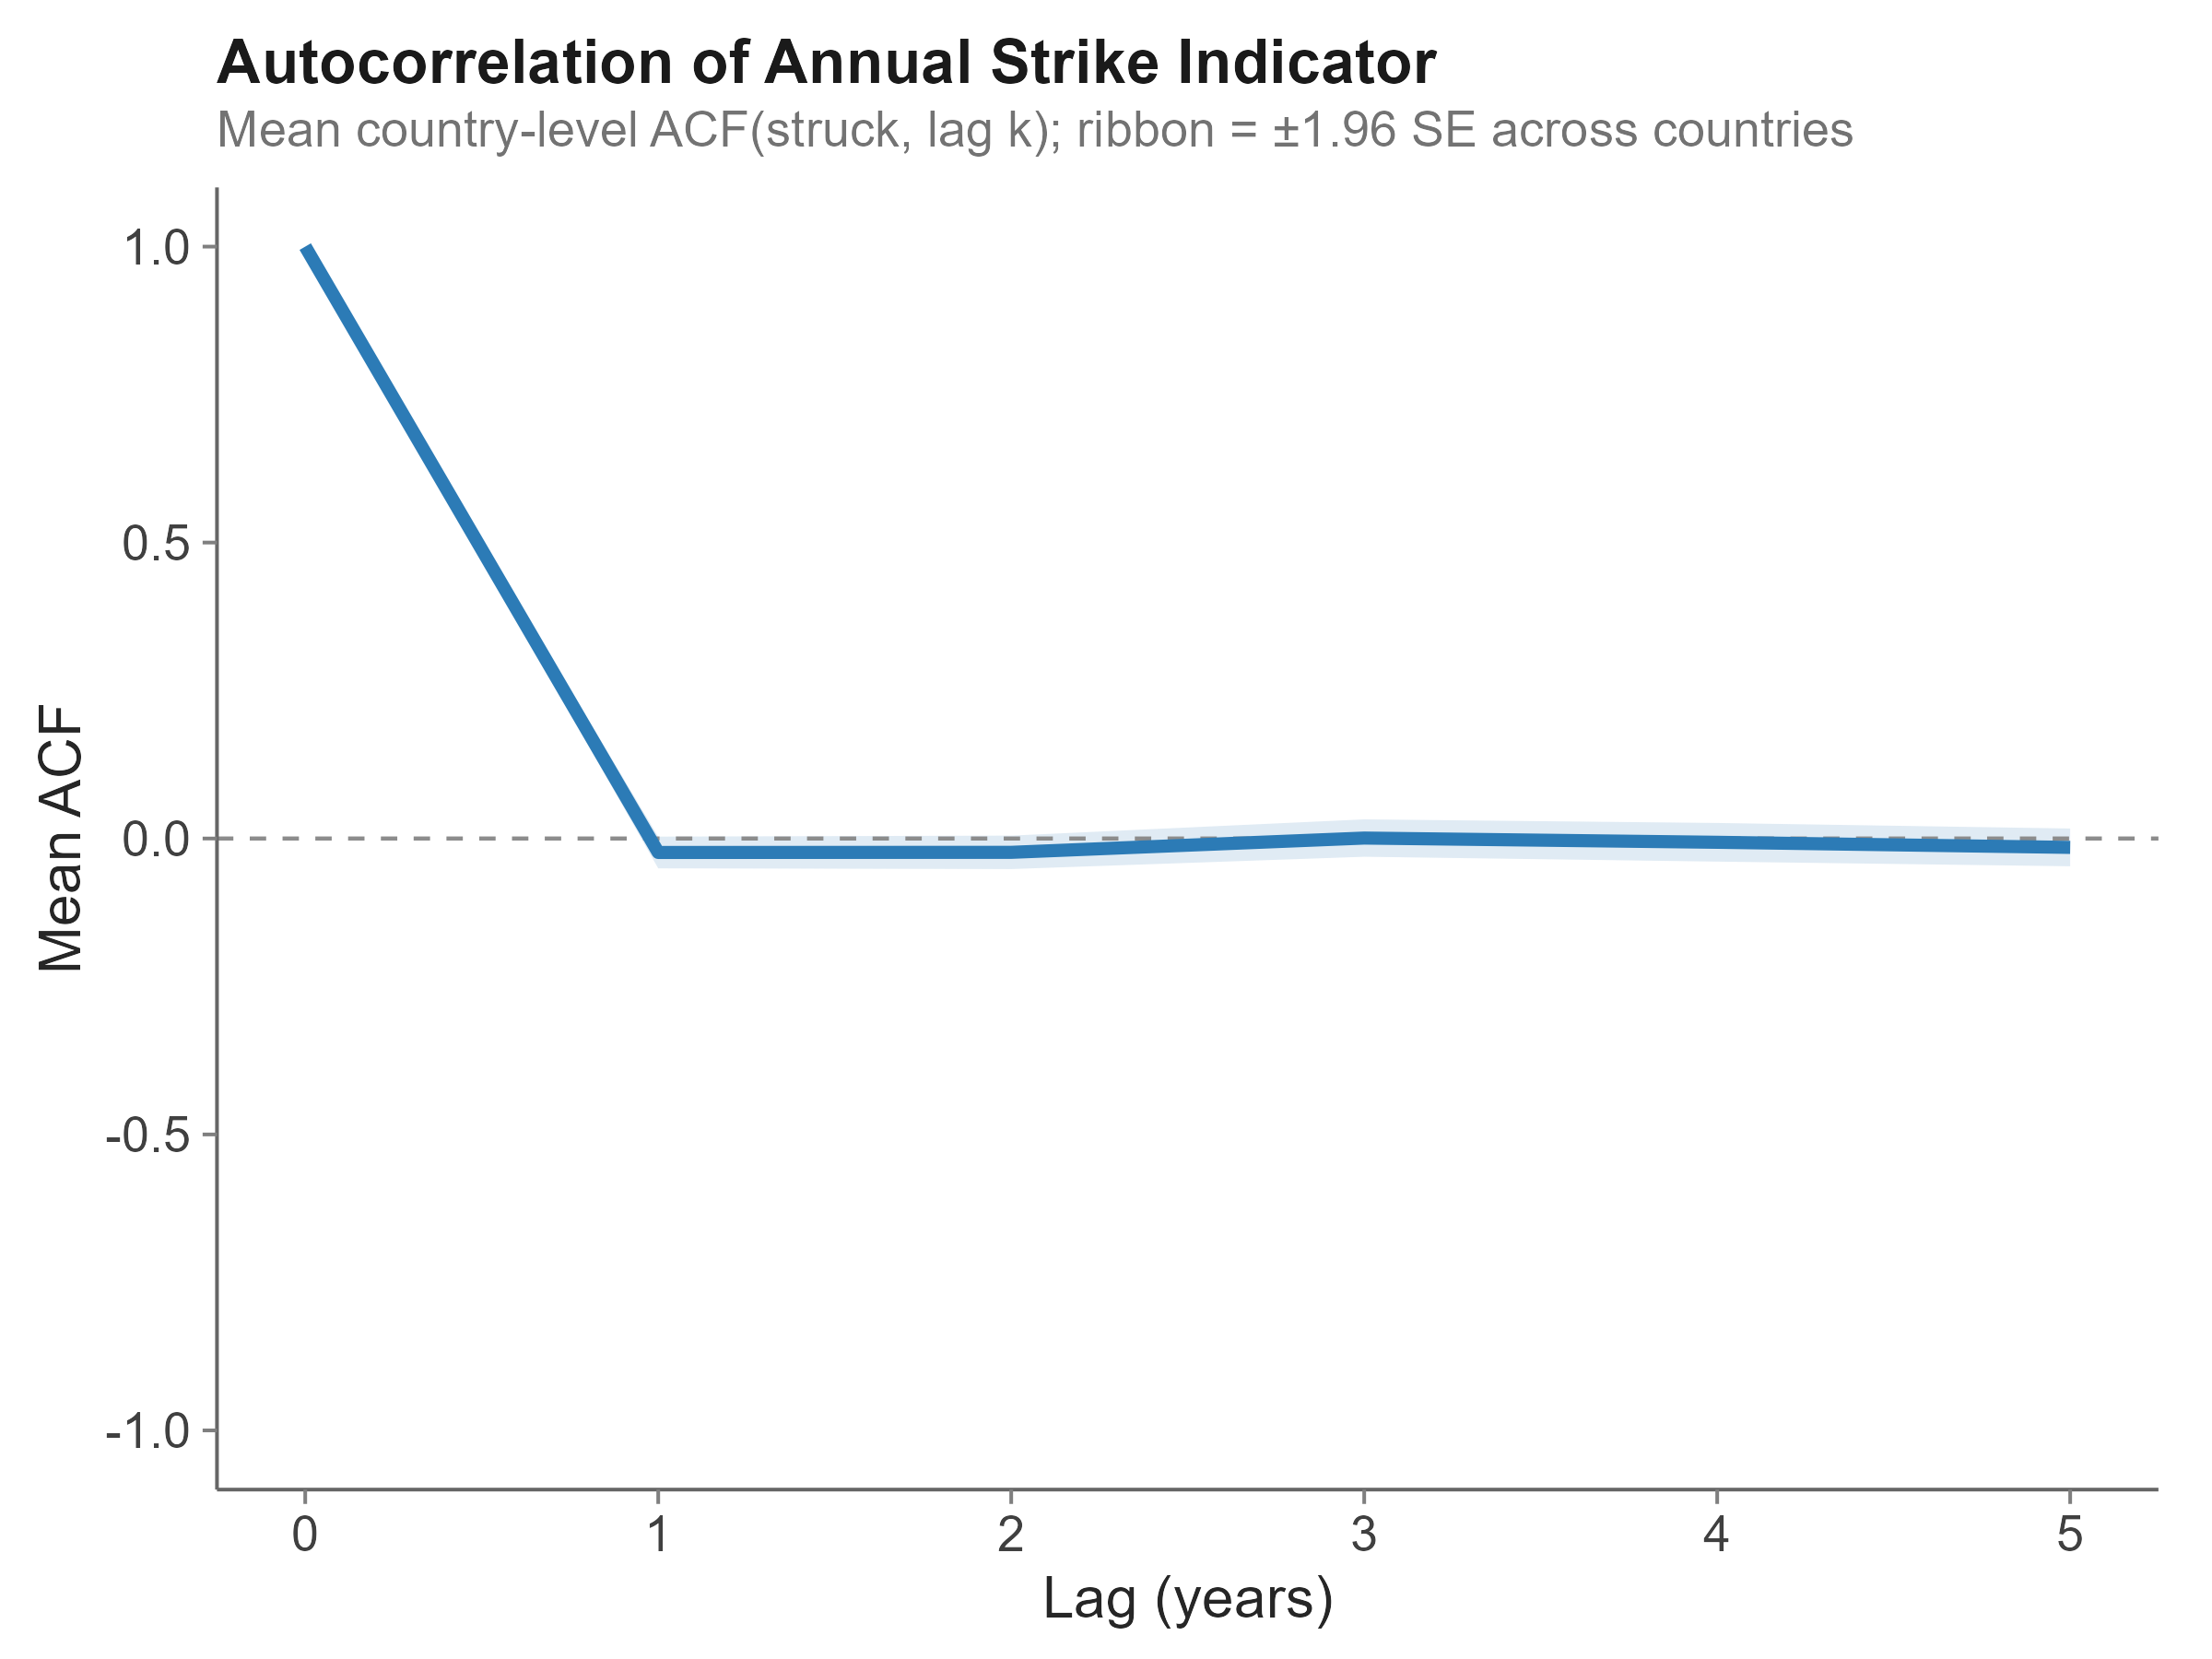
\includegraphics[width=0.82\textwidth,height=0.72\textheight,keepaspectratio]{figures/clim_acf.png}

\smallskip\small
Mean country-level ACF of $\mathbf{1}[\text{maxwind}>0]$, pooled across all countries.
Ribbon = $\pm$1.96\,SE.  Near-zero ACF at all lags supports the i.i.d.-within-country
assumption underlying the LP.
\end{frame}

\begin{frame}{Baseline LP: GDP Response by Country Climatology}
\centering
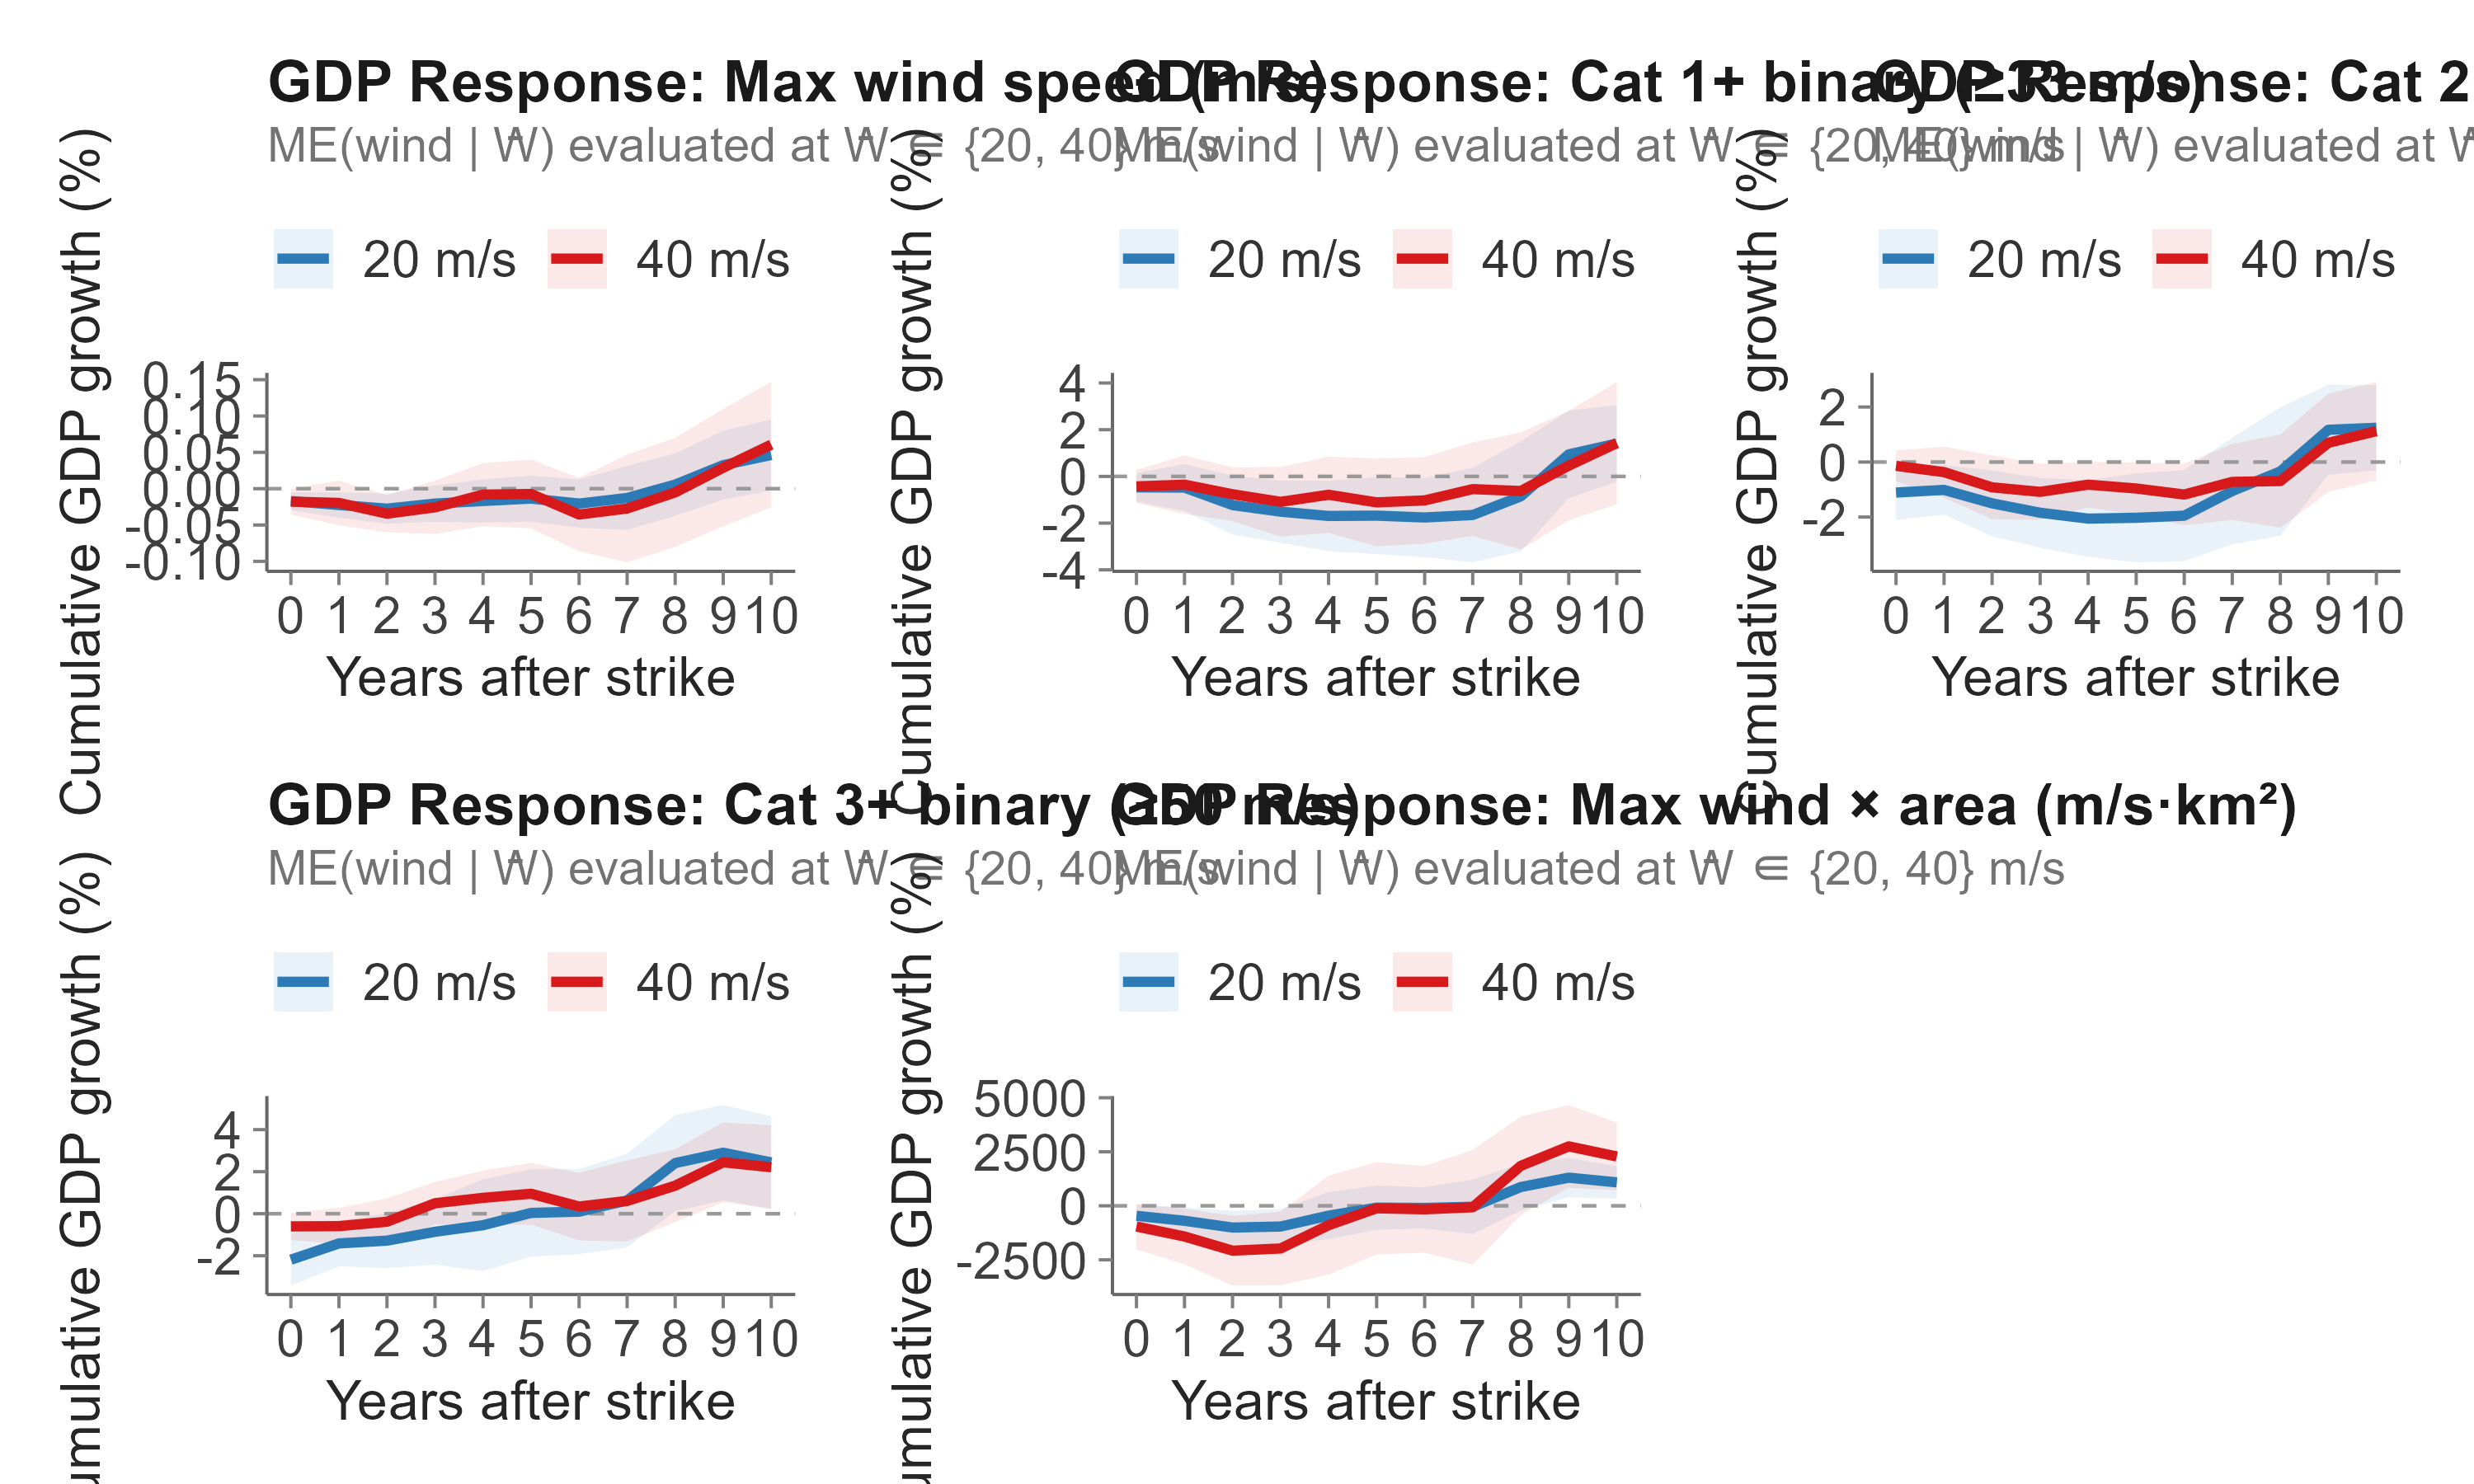
\includegraphics[width=0.96\textwidth,height=0.72\textheight,keepaspectratio]{figures/irf_climatology_all.png}

\smallskip\small
State-dependent LP at $\bar{W}\in\{20,40\}$\,m/s, five shock definitions.
Blue = low-climatology ($\bar{W}=20$), red = high-climatology ($\bar{W}=40$).
This motivates asking whether \emph{recent prior exposure} moderates the response.
\end{frame}

% ===============================================================
\section{The Compound Question and Its Identification Problem}
% ===============================================================
{\hideframenumber\begin{frame}\sectionpage\end{frame}\showframenumber}

\begin{frame}{The Compound Question}
\small
\textbf{Question:} does the GDP cost of a cyclone depend on how recently the
country was last struck?

\smallskip
Two competing stories:

\smallskip
\begin{tabular}{@{}p{4.8cm}p{6.8cm}@{}}
\toprule
Mechanism & Prediction \\
\midrule
\textbf{Compounding damage} \newline
(fiscal space exhausted, \newline infrastructure already damaged)
  & GDP hit is \emph{larger} when the prior strike was recent \\[3pt]
\textbf{Adaptation / reduced stock} \newline
(less capital to destroy,\newline households diversified)
  & GDP hit is \emph{smaller} when the prior strike was recent \\
\bottomrule
\end{tabular}

\smallskip
\textbf{Approach:} estimate
$\text{ME}(w_{it} \mid \tau_{it} = c) = \hat\beta_1 + \hat\beta_2\cdot c$
where $\tau_{it}$ = years since the country's previous TC event.

\smallskip
\textbf{The identification problem:} $\tau_{it}$ is not randomly assigned.
\normalsize
\end{frame}

\begin{frame}{Why $\tau$ Is Not Randomly Assigned}

\textbf{Mechanical link:} a country with high average wind climatology
$\bar{W}_i$ is struck \emph{more often} $\Rightarrow$ it has shorter
inter-strike gaps $\tau$ on average --- by construction.

\medskip
Formally, the state variable $\tau_{it}$ is a function of past shocks:
\[
  \tau_{it} = t - \max\bigl\{s < t : w_{is} > 0\bigr\}
\]
Its distribution depends on the Bernoulli success probability
$p_i = P(\text{struck}_t)$, which is a monotone function of $\bar{W}_i$.

\medskip
\textbf{Consequence:} if we find that the GDP response is larger when $\tau$
is large (isolated event), we cannot immediately conclude this is a
\emph{time-since-last-strike} effect.  It could instead be:
\begin{itemize}
  \item A \textbf{cross-country adaptation effect}: isolated events happen
        disproportionately in low-$\bar{W}$ countries, which are less
        adapted.
  \item A \textbf{selection effect}: never-struck periods are more common
        for rarely-struck countries.
\end{itemize}

\medskip
$\Rightarrow$ We need to establish this empirically and then design robustness
tests.
\end{frame}

\begin{frame}{EDA: High-Climatology Countries Have Shorter Inter-Strike Gaps}
\centering
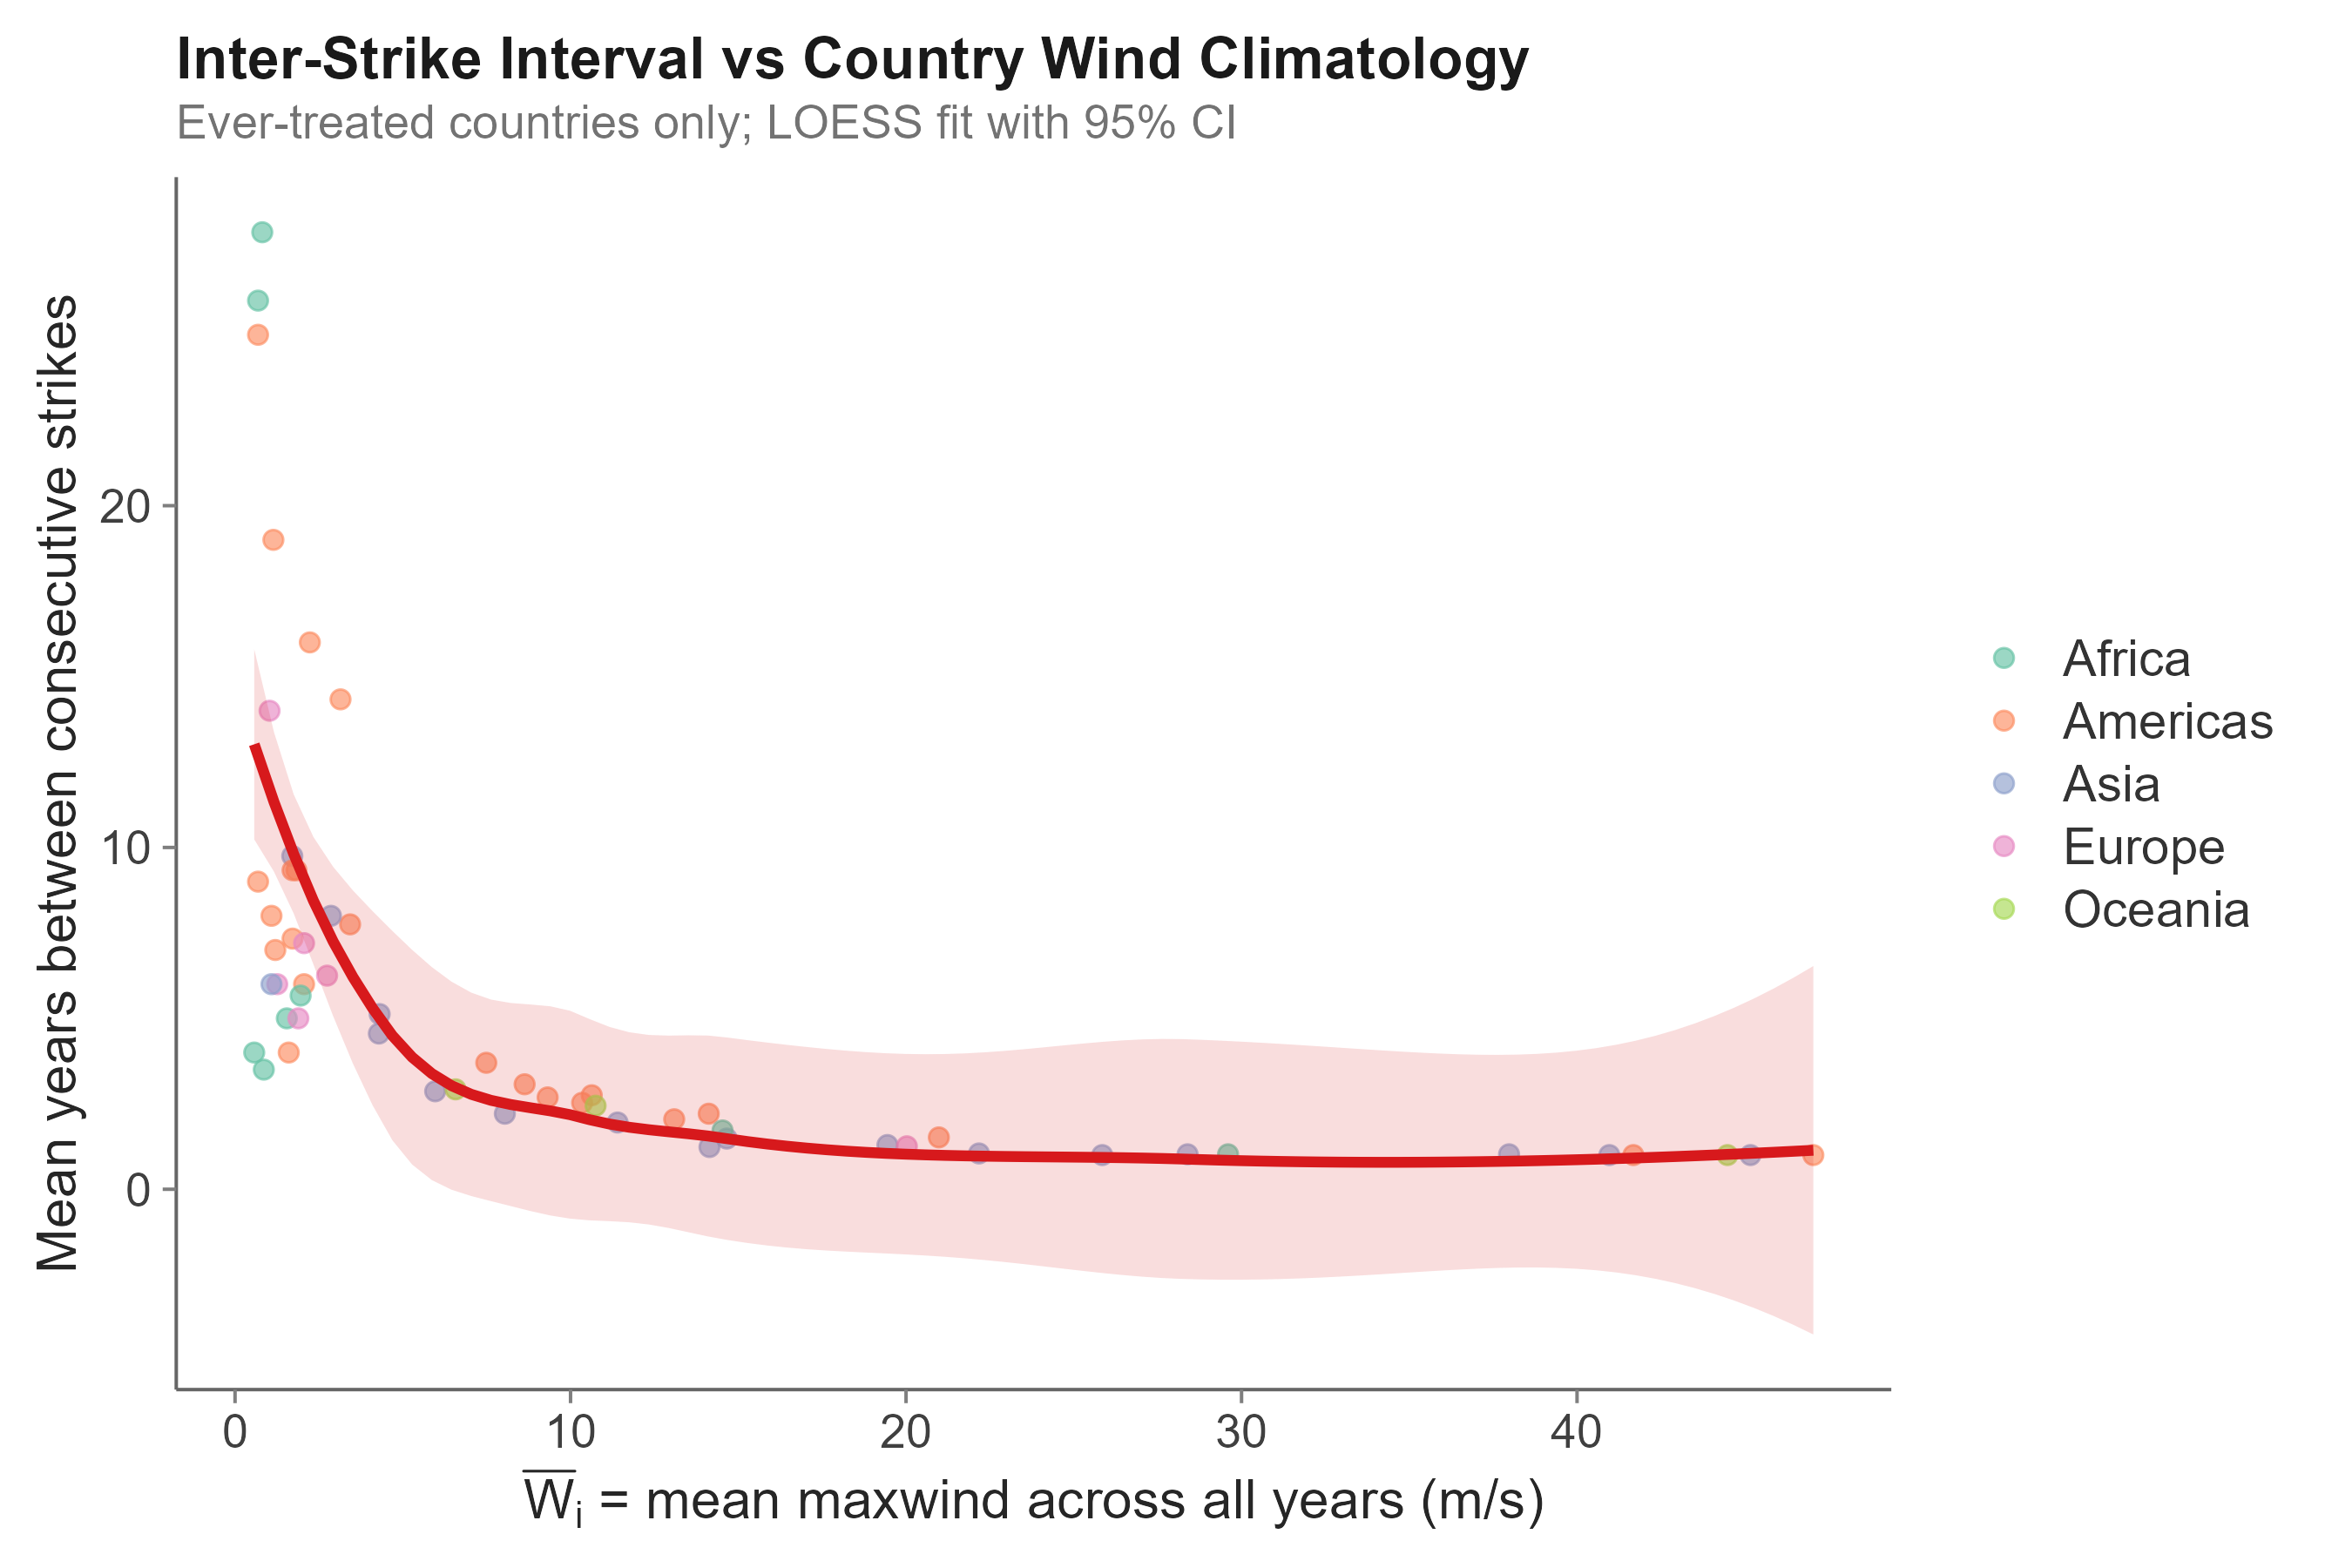
\includegraphics[width=0.88\textwidth,height=0.70\textheight,keepaspectratio]{figures/clim_gap_vs_wbar.png}

\smallskip\small
Ever-treated countries ($\bar{W}_i>0$).  X: $\bar{W}_i$ (m/s).  Y: mean years between strikes.
LOESS fit $\pm$95\,\% CI.  Higher $\bar{W}$ $\Rightarrow$ shorter gaps $\Rightarrow$ lower $\tau$.
This is mechanical, not behavioural.
\end{frame}

\begin{frame}{EDA: Compound Events Cluster in High-Climatology Countries}
\centering
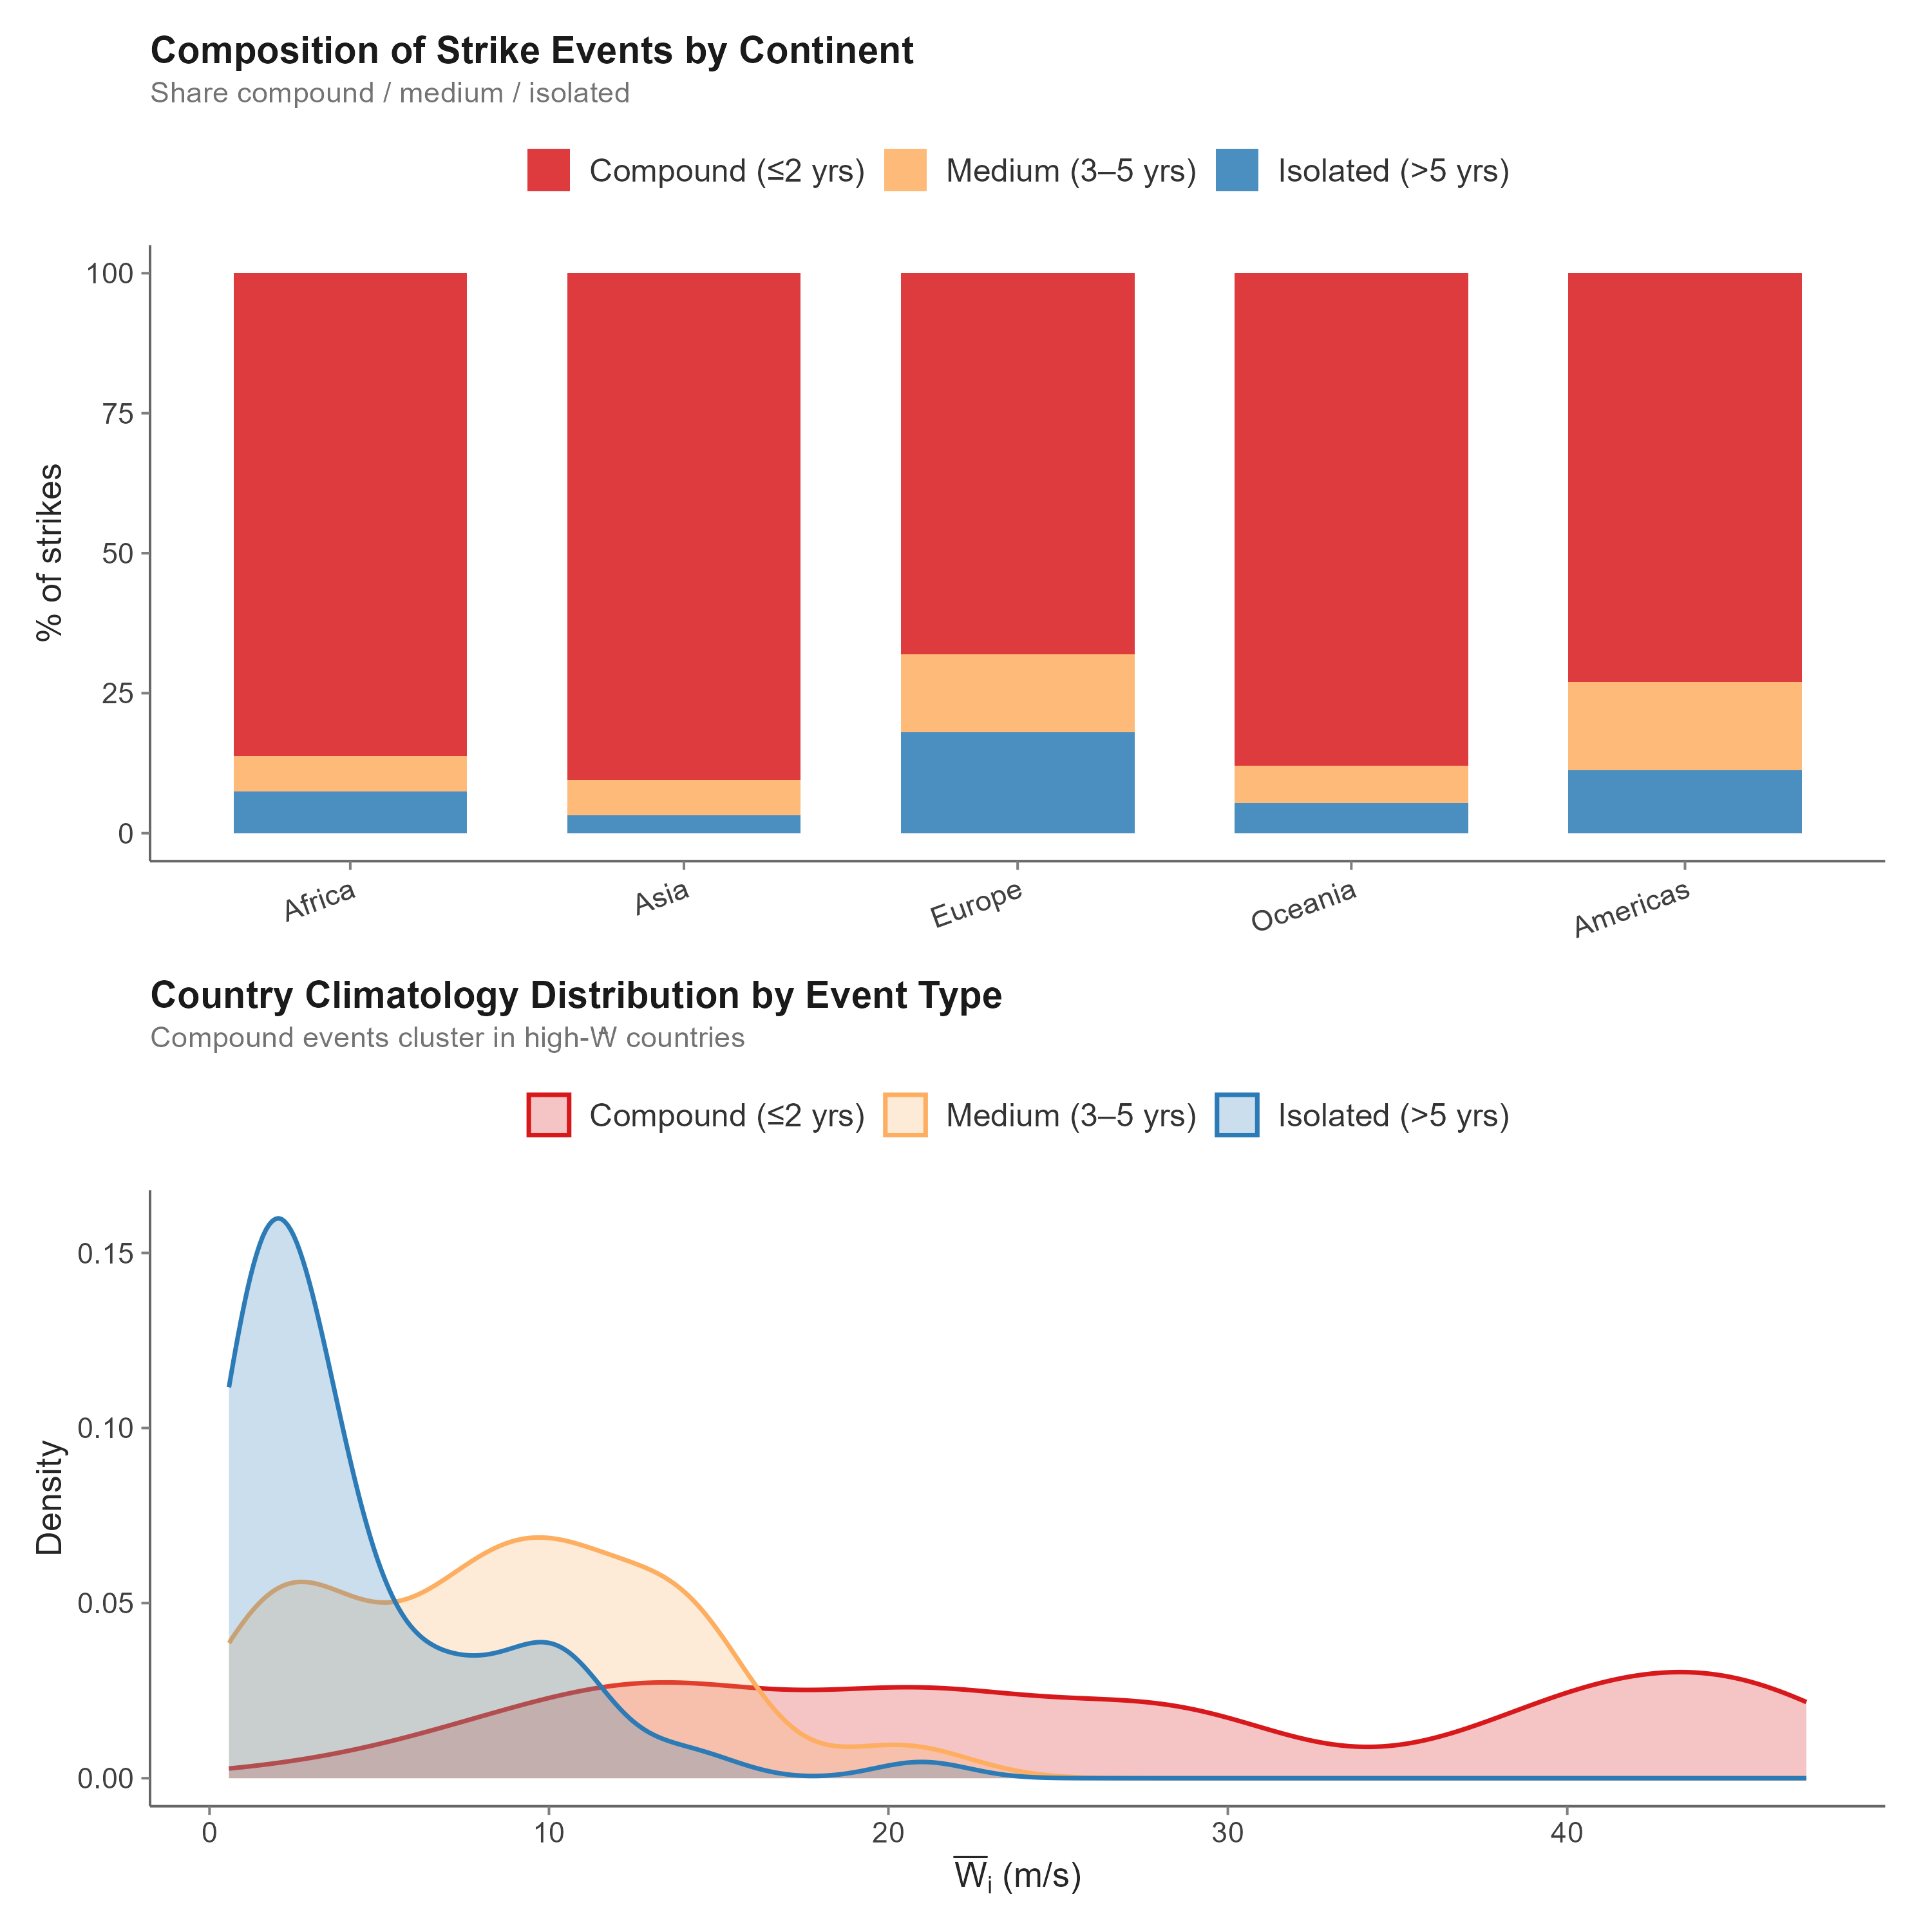
\includegraphics[width=0.96\textwidth,height=0.68\textheight,keepaspectratio]{figures/compound_rob_descriptive.png}

\smallskip\small
\textbf{Top:} share of compound ($\tau\leq2$), medium ($\tau\in[3,5]$), and isolated ($\tau>5$) events by continent.
\textbf{Bottom:} $\bar{W}_i$ distribution by event type --- compound events cluster in high-climatology countries.
$\tau$ and $\bar{W}$ are strongly correlated: any compound-LP gradient partially reflects the climatology gradient.
\end{frame}

\begin{frame}{Back-to-Back Strikes: Rate by Climatology Decile}
\centering
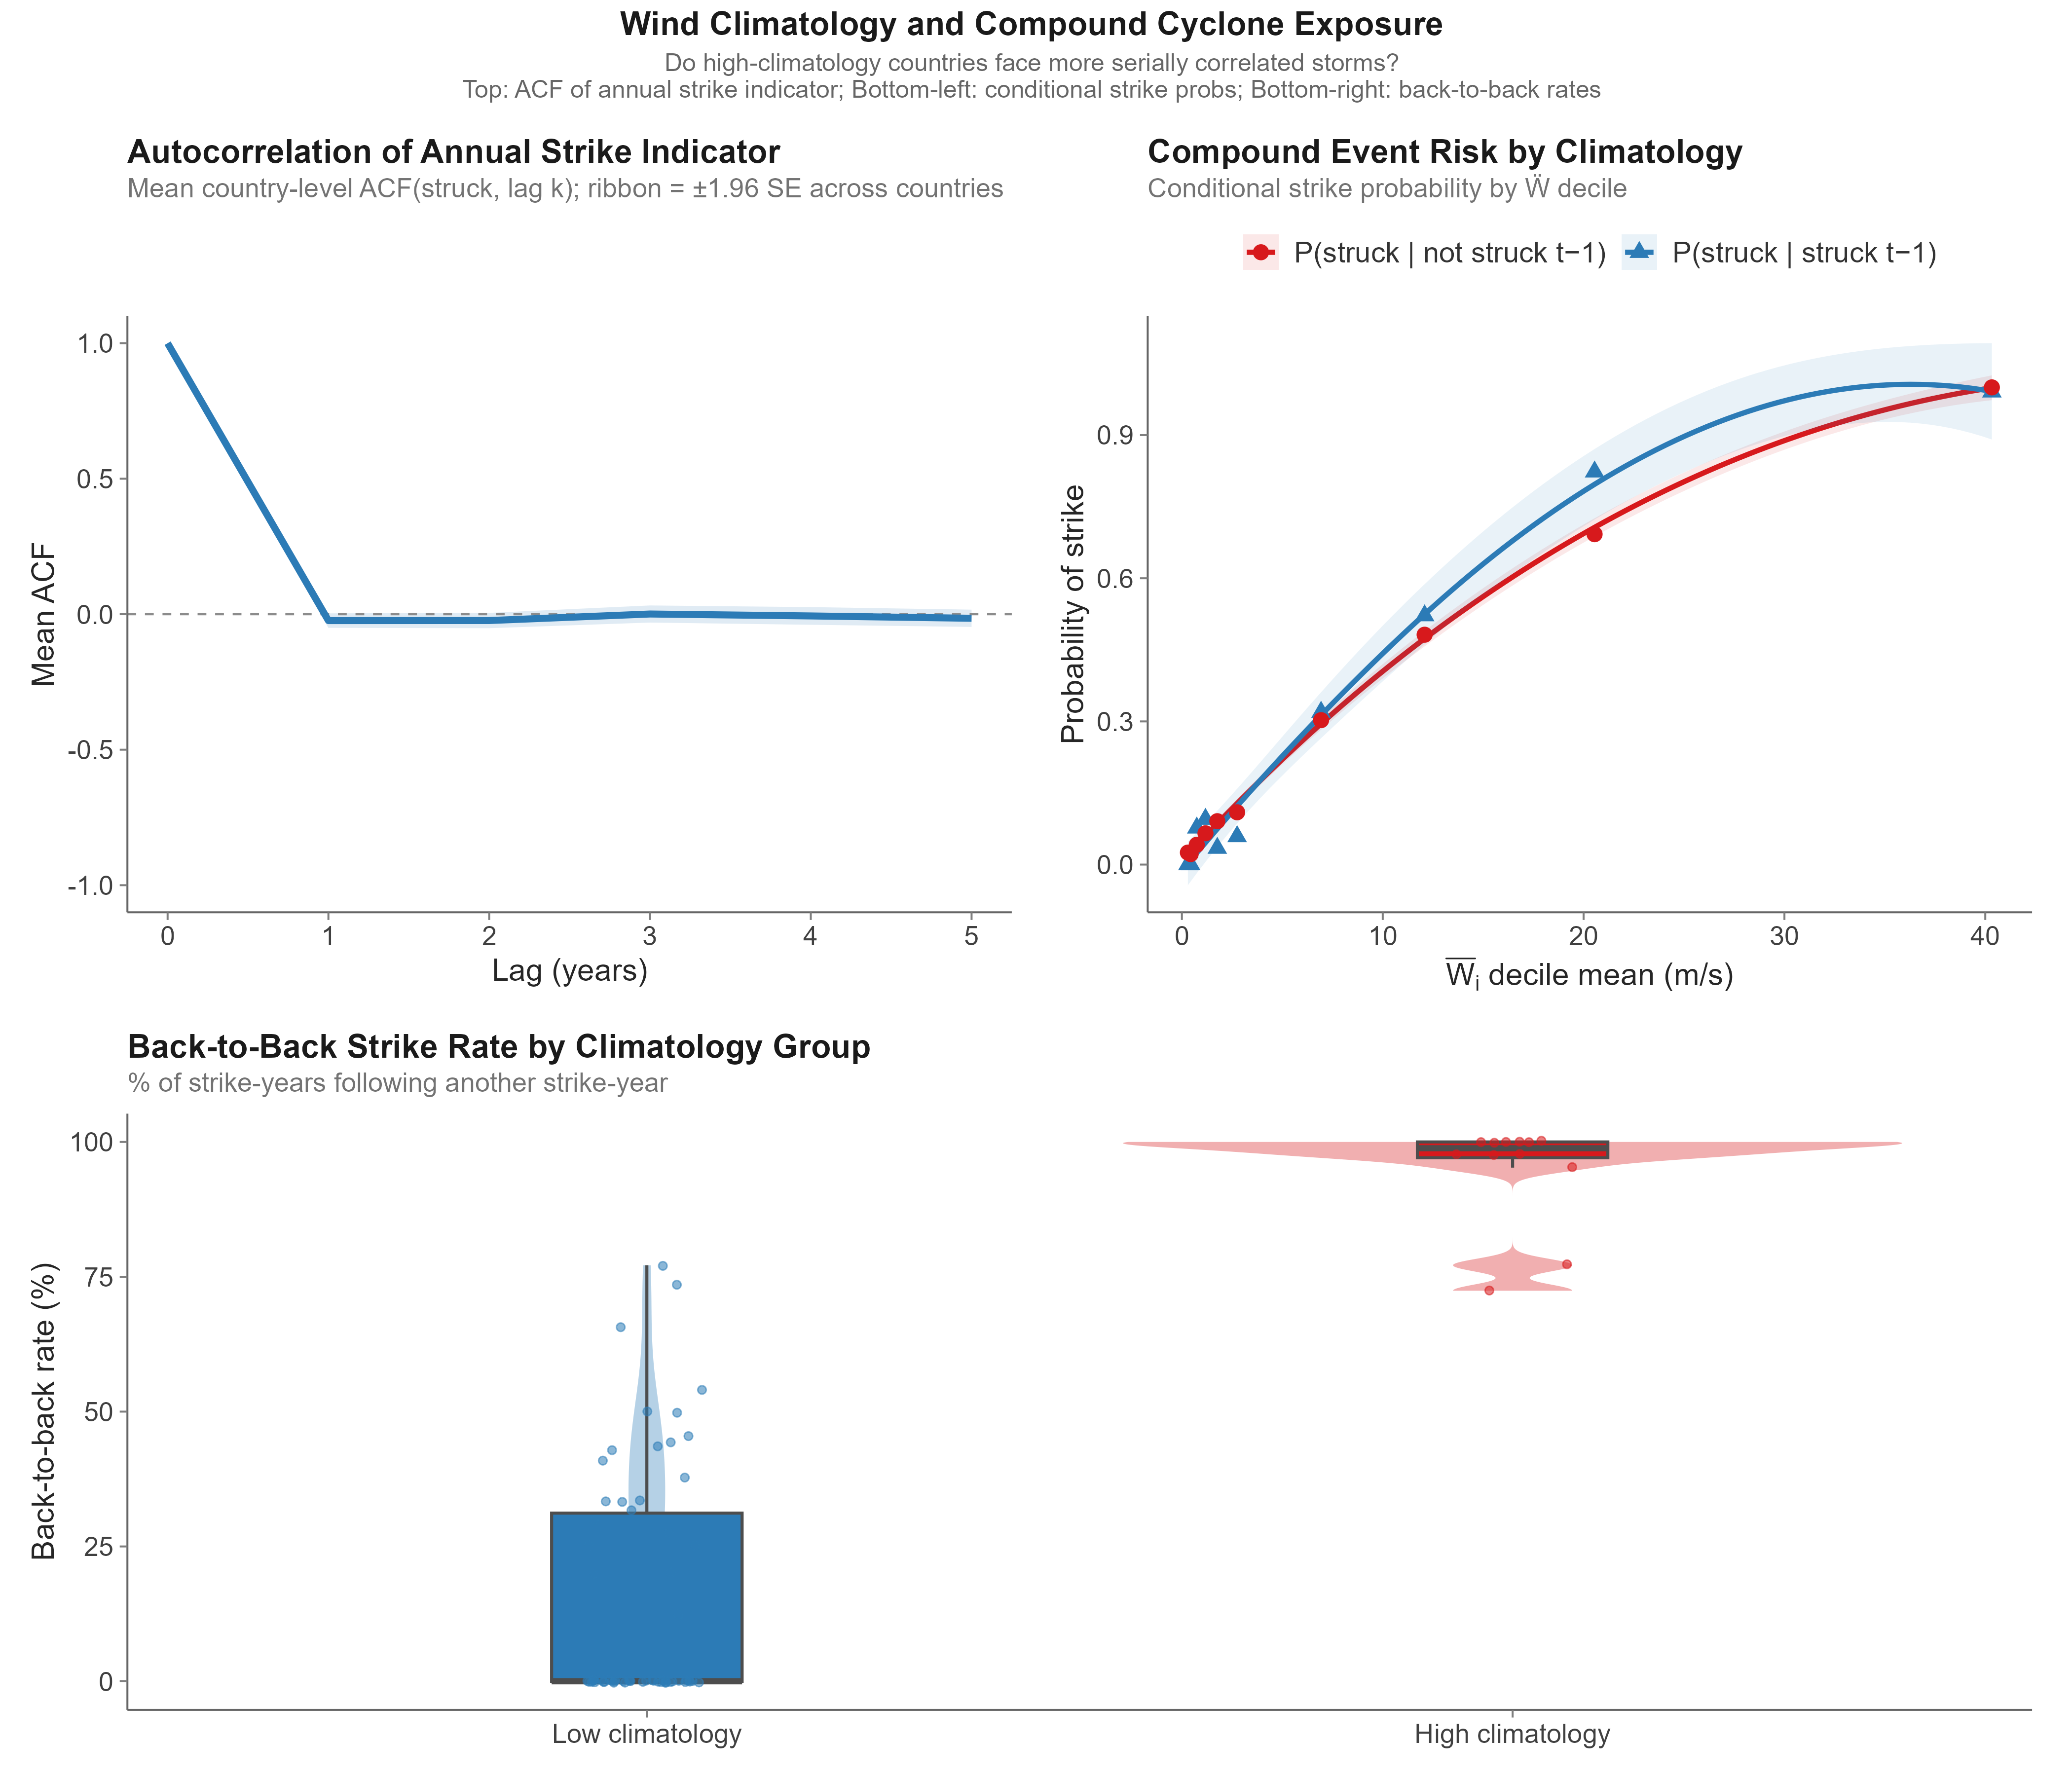
\includegraphics[width=0.96\textwidth,height=0.72\textheight,keepaspectratio]{figures/clim_compound_combined.png}

\smallskip\small
\textbf{Left:} $P(\text{struck}_t\mid\text{struck}_{t-1})$ vs.\ $P(\text{struck}_t\mid\text{not struck}_{t-1})$ by $\bar{W}$ decile.
\textbf{Right:} back-to-back strike rate by climatology group.
High-$\bar{W}$ countries have substantially elevated compound probabilities --- $\tau$ is not randomly assigned.
\end{frame}

\begin{frame}{Identification Summary}

\begin{tabular}{@{}p{5cm}p{3.2cm}p{3.5cm}@{}}
\toprule
Object & Randomly assigned? & Identification lever \\
\midrule
$w_{it}$ (maxwind in year $t$) & \textbf{Yes}, conditional on $\bar{W}_i$ and FEs
  & Within-country year-to-year variation \\[4pt]
$\bar{W}_i$ (long-run climatology) & No --- time-invariant geography
  & Cross-country; absorbed by FE as level \\[4pt]
$\tau_{it}$ (years since last TC) & \textbf{No} --- determined by history of $w_{is}$;
  systematically shorter for high-$\bar{W}_i$ countries
  & Cannot be isolated from $\bar{W}_i$ without further assumptions \\
\bottomrule
\end{tabular}

\medskip\small
The compound LP estimates
$\beta_1 + \beta_2\cdot\tau$ but $\beta_2$ conflates the
\emph{time-since-last-event} mechanism with the cross-sectional
\emph{adaptation-to-climatology} mechanism.
Robustness tests (within-climatology splits, LOCO, ever-treated) probe
the severity of this confound; a valid IV would solve it.
\end{frame}

% ===============================================================
\section{Compound LP: Specification and Methods}
% ===============================================================
{\hideframenumber\begin{frame}\sectionpage\end{frame}\showframenumber}

\begin{frame}{Compound LP: The Model}

\small For each horizon $h = 0, \ldots, 10$, estimate by OLS:
\[
  \log\text{GDP}_{i,t+h} - \log\text{GDP}_{i,t-1}
  = \beta_1^{(h)}\, w_{it}
  + \beta_2^{(h)} (w_{it} \times \tau_{it})
  + \boldsymbol{\gamma}^{(h)\prime} X_{it}
  + \alpha_i^{(h)}(t) + \delta_{r(i)t}^{(h)} + \varepsilon_{iht}
\]

\vspace{-4pt}
\begin{tabular}{@{}lp{8.5cm}@{}}
\toprule
Symbol & Definition \\
\midrule
$w_{it}$ & Shock variable (five variants) \\
$\tau_{it}$ & Years since last maxwind\,$>0$ (continuous state variable) \\
$X_{it}$ & $\ell(w_{it},1{:}2)$ and $\ell(\Delta\log\text{GDP}_{it},1{:}2)$
           (two lags of shock and GDP growth) \\
$\alpha_i^{(h)}(t)$ & Country quadratic trend (\texttt{countrycode[year] + countrycode[year\textsuperscript{2}]}) \\
$\delta_{r(i)t}^{(h)}$ & Region$\times$year FE (\texttt{region\^{}year}) \\
\bottomrule
\end{tabular}

\vspace{-2pt}
\textbf{Marginal effect} at $\tau = c$ (delta-method SE):
\[
  \widehat{\text{ME}}(c) = \hat\beta_1^{(h)} + \hat\beta_2^{(h)}\cdot c,
  \quad
  \widehat{\text{SE}}(c) = \sqrt{\hat V_{11} + c^2 \hat V_{22} + 2c\,\hat V_{12}}
\]
Evaluated at $c \in \{1,\,3,\,5\}$ years.
\normalsize
\end{frame}

\begin{frame}{Methods: State Variable, Residualisation, and SE}
\small
\textbf{1.\ State variable} (\texttt{time\_since\_last}):
$\tau_{it} = t - \max\{s < t : w_{is} > 0\}$;
\texttt{NA} before the first ever strike.  At the strike year, $\tau$ records
the gap since the \emph{previous} strike, not zero.

\smallskip
\textbf{2.\ Residualised shock:}
$\tilde{w}_{it} = \text{maxwind}_{it} - \hat\mu_{it}$ where
$\hat\mu_{it}$ from \texttt{feols(maxwind\,$\sim$\,1\,|\,countrycode[year]\,+\,region\^{}year)}.
Removes country linear trends and region$\times$year patterns;
retains idiosyncratic wind variation ($\text{cor}\approx0.52$).

\smallskip
\textbf{3.\ SE:} Driscoll--Kraay (\texttt{vcov = DK \textasciitilde\ year}) ---
arbitrary serial correlation within country and spatial correlation across
countries in the same year.

\smallskip
\textbf{4.\ Five shock variables}, all interacted with $\tau^{\text{any}}$:

\smallskip
\begin{tabular}{@{}llr@{}}
\toprule
Name & \texttt{R} variable & Threshold \\
\midrule
Raw maxwind         & \texttt{maxwind}       & continuous (m/s) \\
Residualised maxwind & \texttt{maxwind\_resid} & net of trends/FEs \\
Cat\,1+ binary      & \texttt{wind\_cat1plus} & $\geq$33\,m/s \\
Cat\,2+ binary      & \texttt{wind\_cat2plus} & $\geq$43\,m/s \\
Cat\,3+ binary      & \texttt{wind\_cat3plus} & $\geq$50\,m/s \\
\bottomrule
\end{tabular}
\normalsize
\end{frame}

% ===============================================================
\section{Results: IRFs Across Five Shock Measures}
% ===============================================================
{\hideframenumber\begin{frame}\sectionpage\end{frame}\showframenumber}

\begin{frame}{IRF: Raw Maxwind $\times$ Time Since Last TC}
\centering
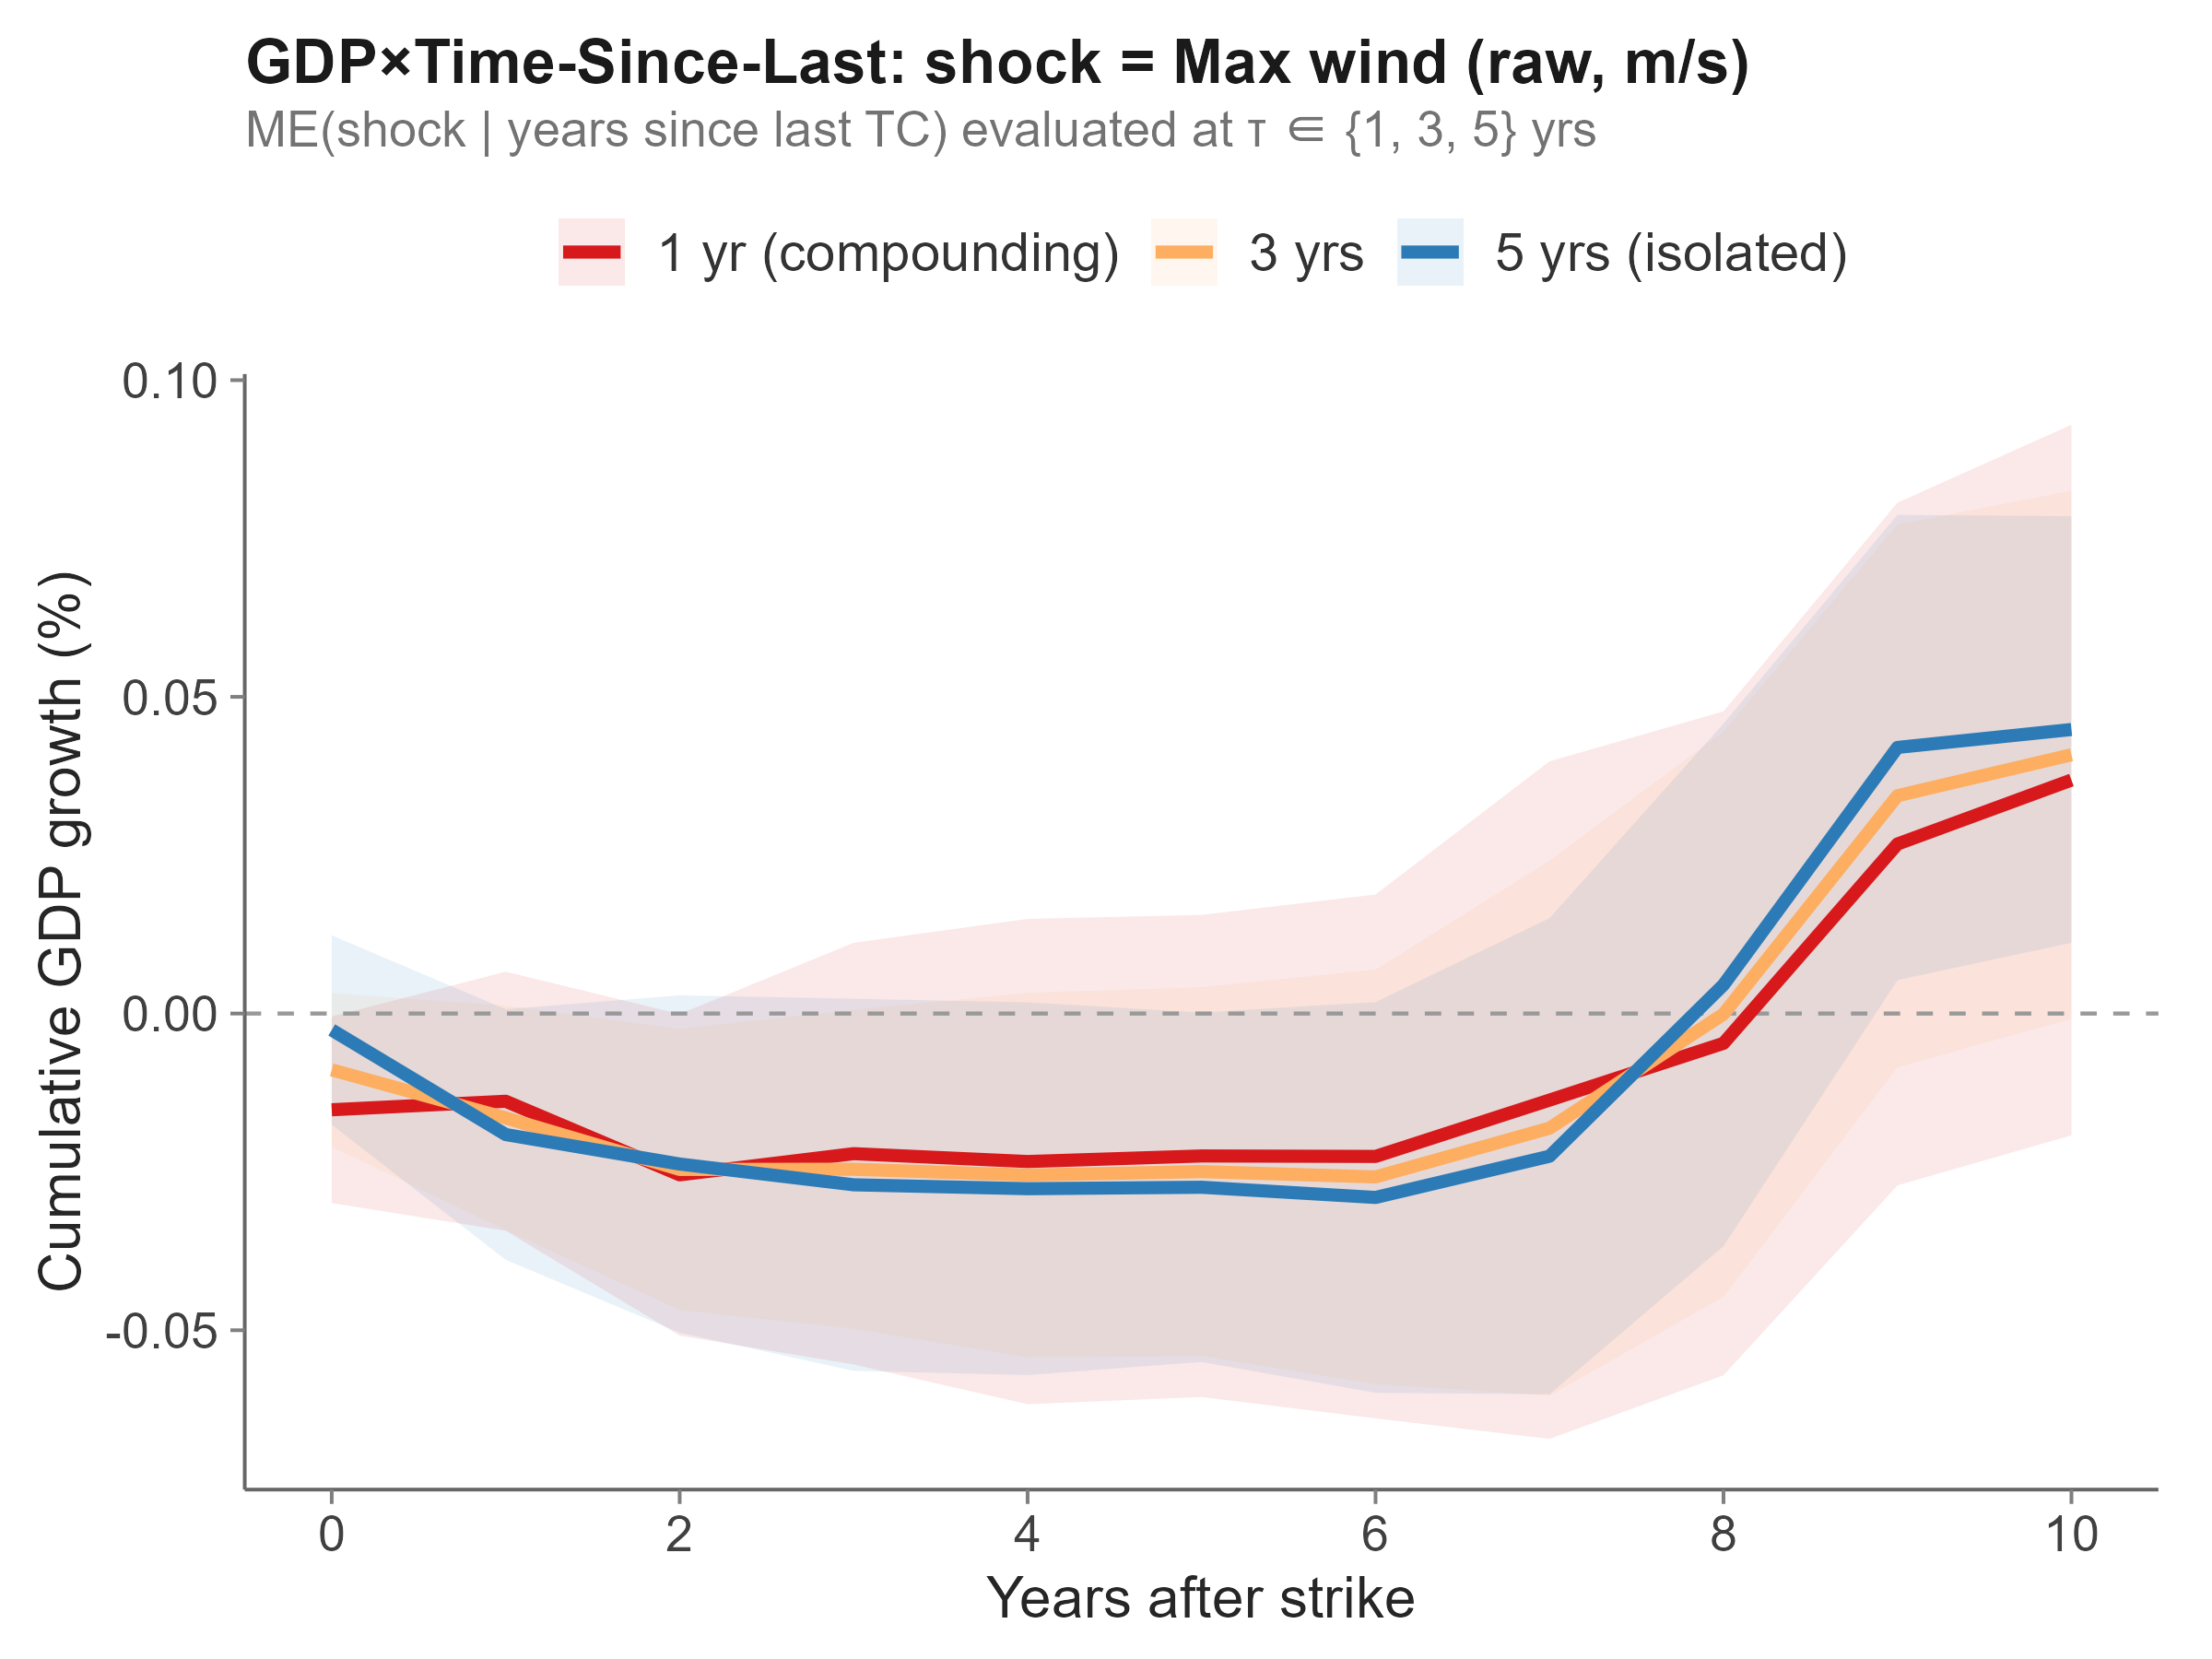
\includegraphics[width=0.82\textwidth,height=0.72\textheight,keepaspectratio]{figures/irf_compound_maxwind.png}

\smallskip\small
Shock = raw max wind speed (m/s).
Red = compounding ($\tau=1$ yr), gold = medium gap ($\tau=3$ yrs),
blue = isolated ($\tau=5$ yrs).
Gradient: isolated events generate slightly larger negative GDP effects,
consistent with both the adaptation and the $\bar{W}$ confound stories.
\end{frame}

\begin{frame}{IRF: Residualised Maxwind $\times$ Time Since Last TC}
\centering
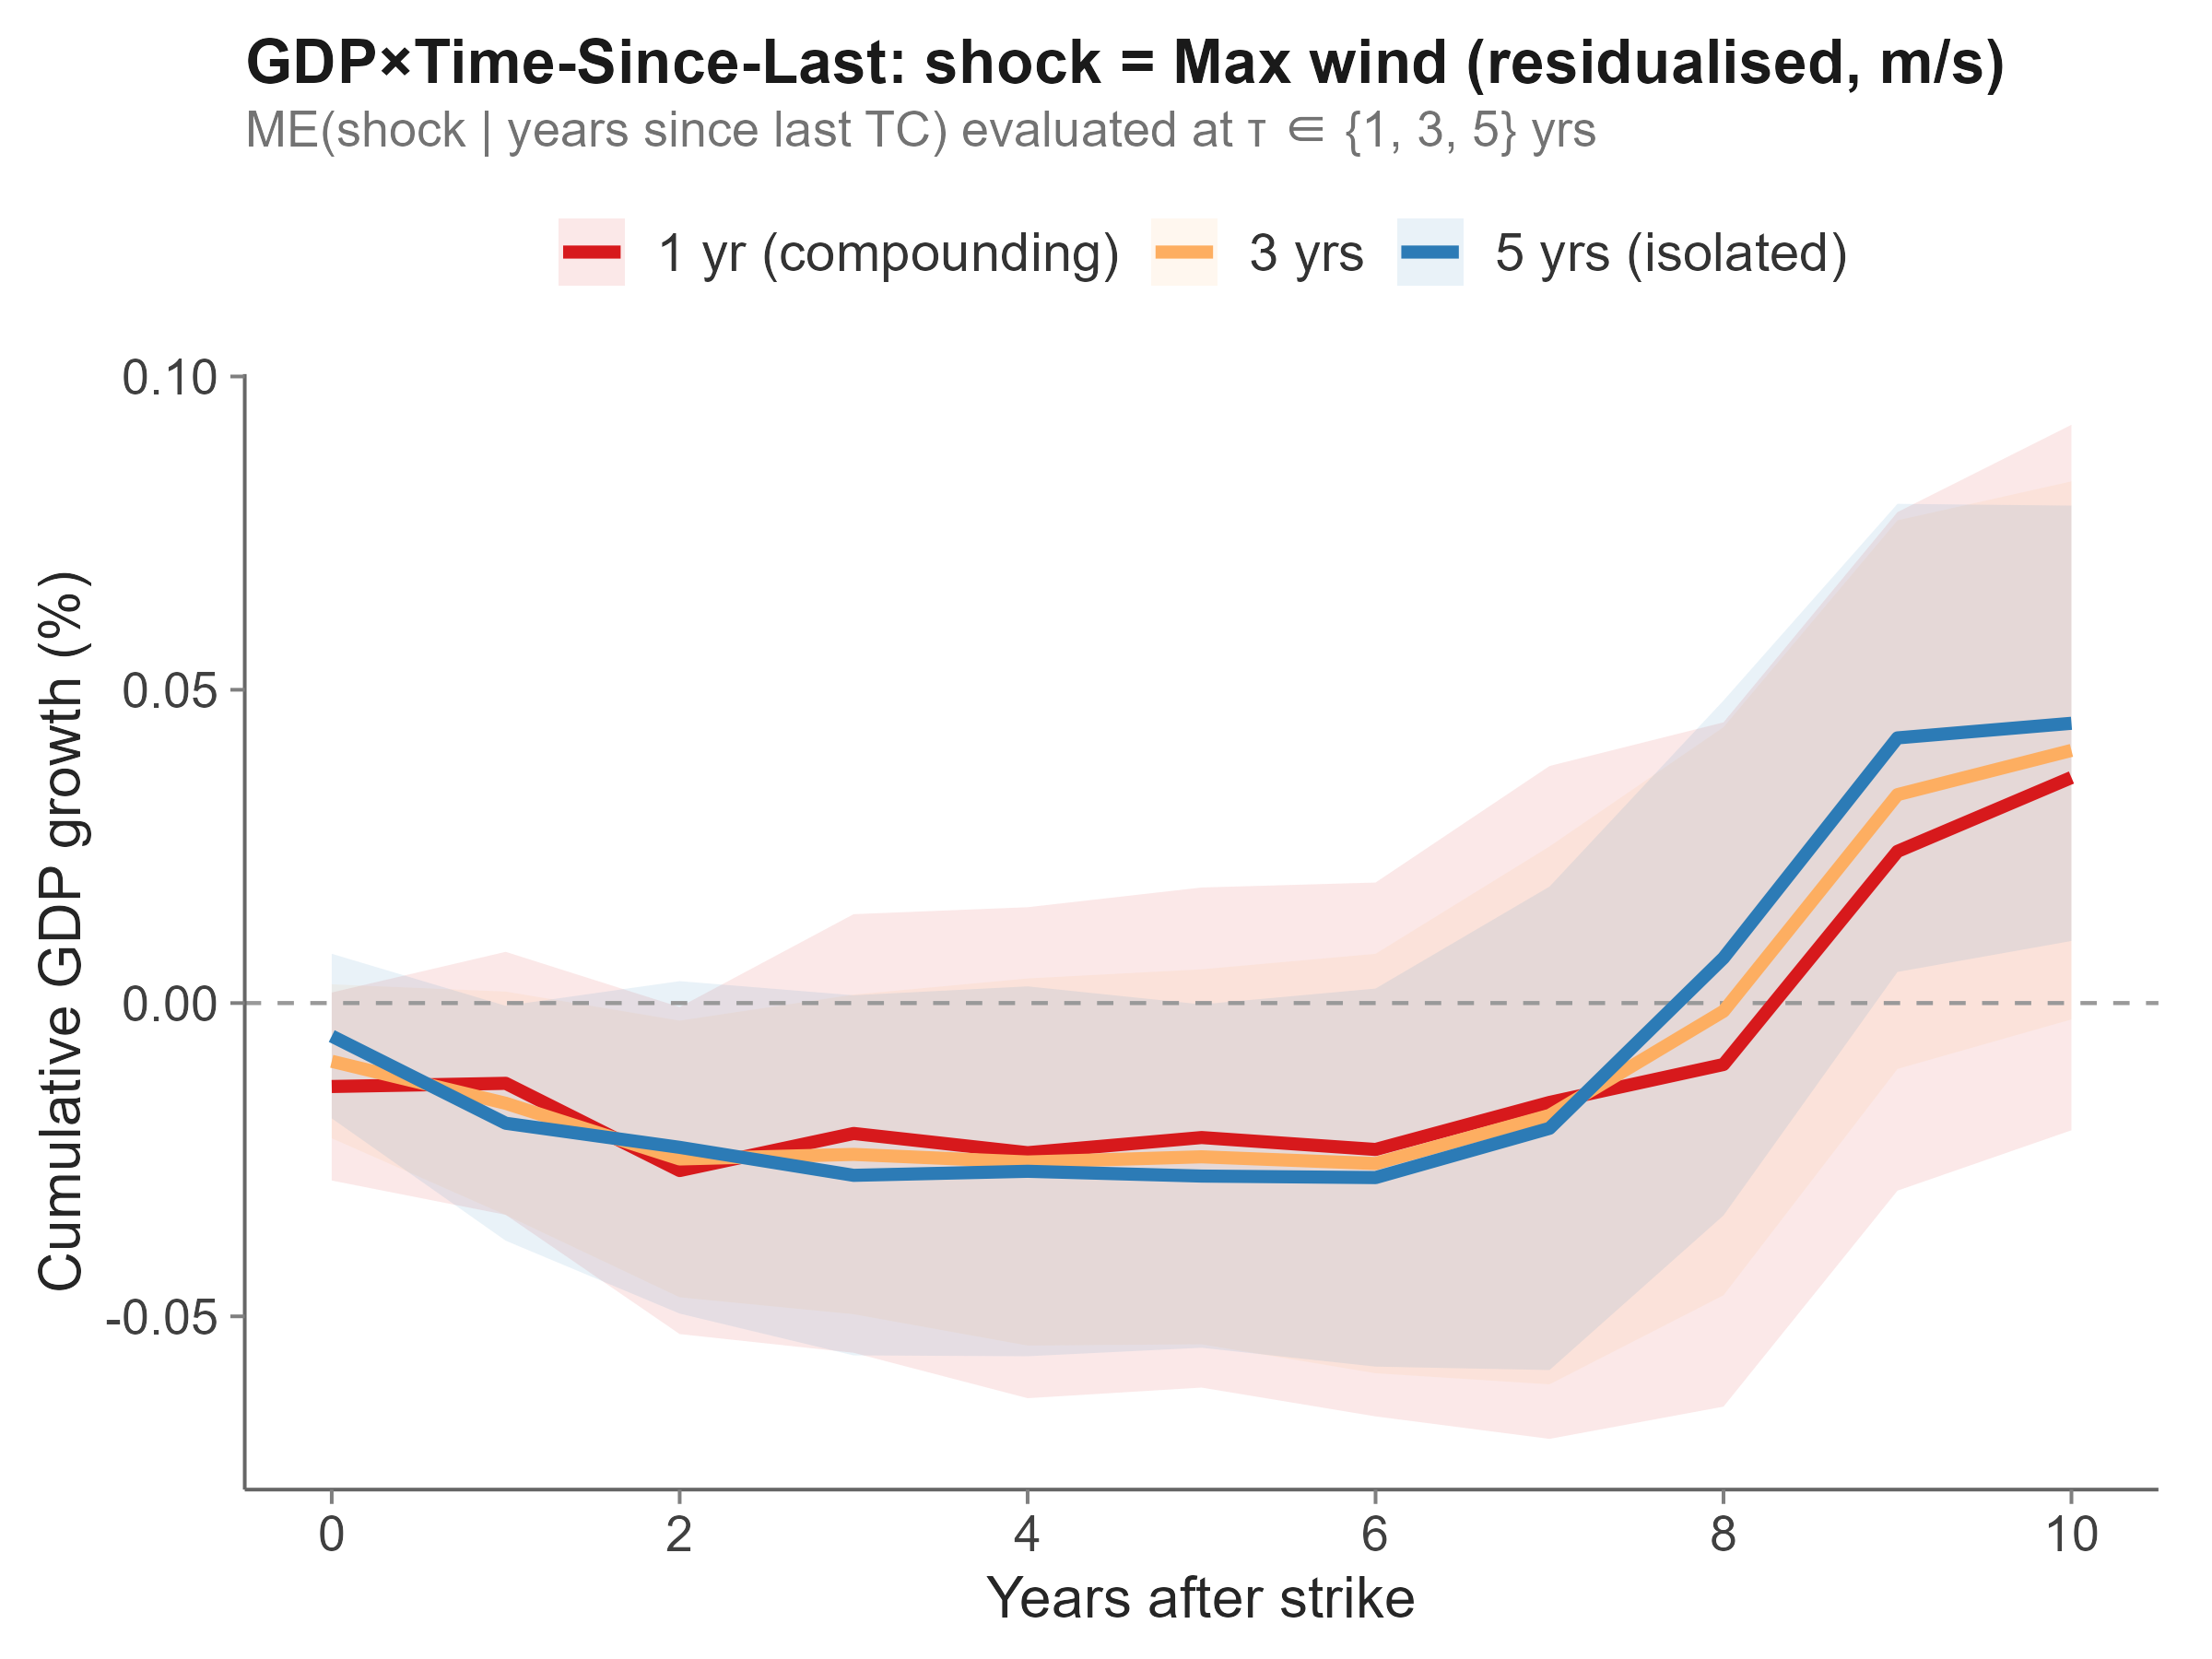
\includegraphics[width=0.82\textwidth,height=0.72\textheight,keepaspectratio]{figures/irf_compound_maxwind_resid.png}

\smallskip\small
Shock = $\tilde{w}_{it}$ (maxwind net of country linear trend and region$\times$year
FE; $\text{cor}\approx0.52$ with raw maxwind).  Residualisation isolates
idiosyncratic within-country wind variation.  Gradient largely unchanged,
suggesting the confound is not driven by predictable cyclone-season patterns.
\end{frame}

\begin{frame}{IRF: Cat\,1+ Binary $\times$ Time Since Last TC}
\centering
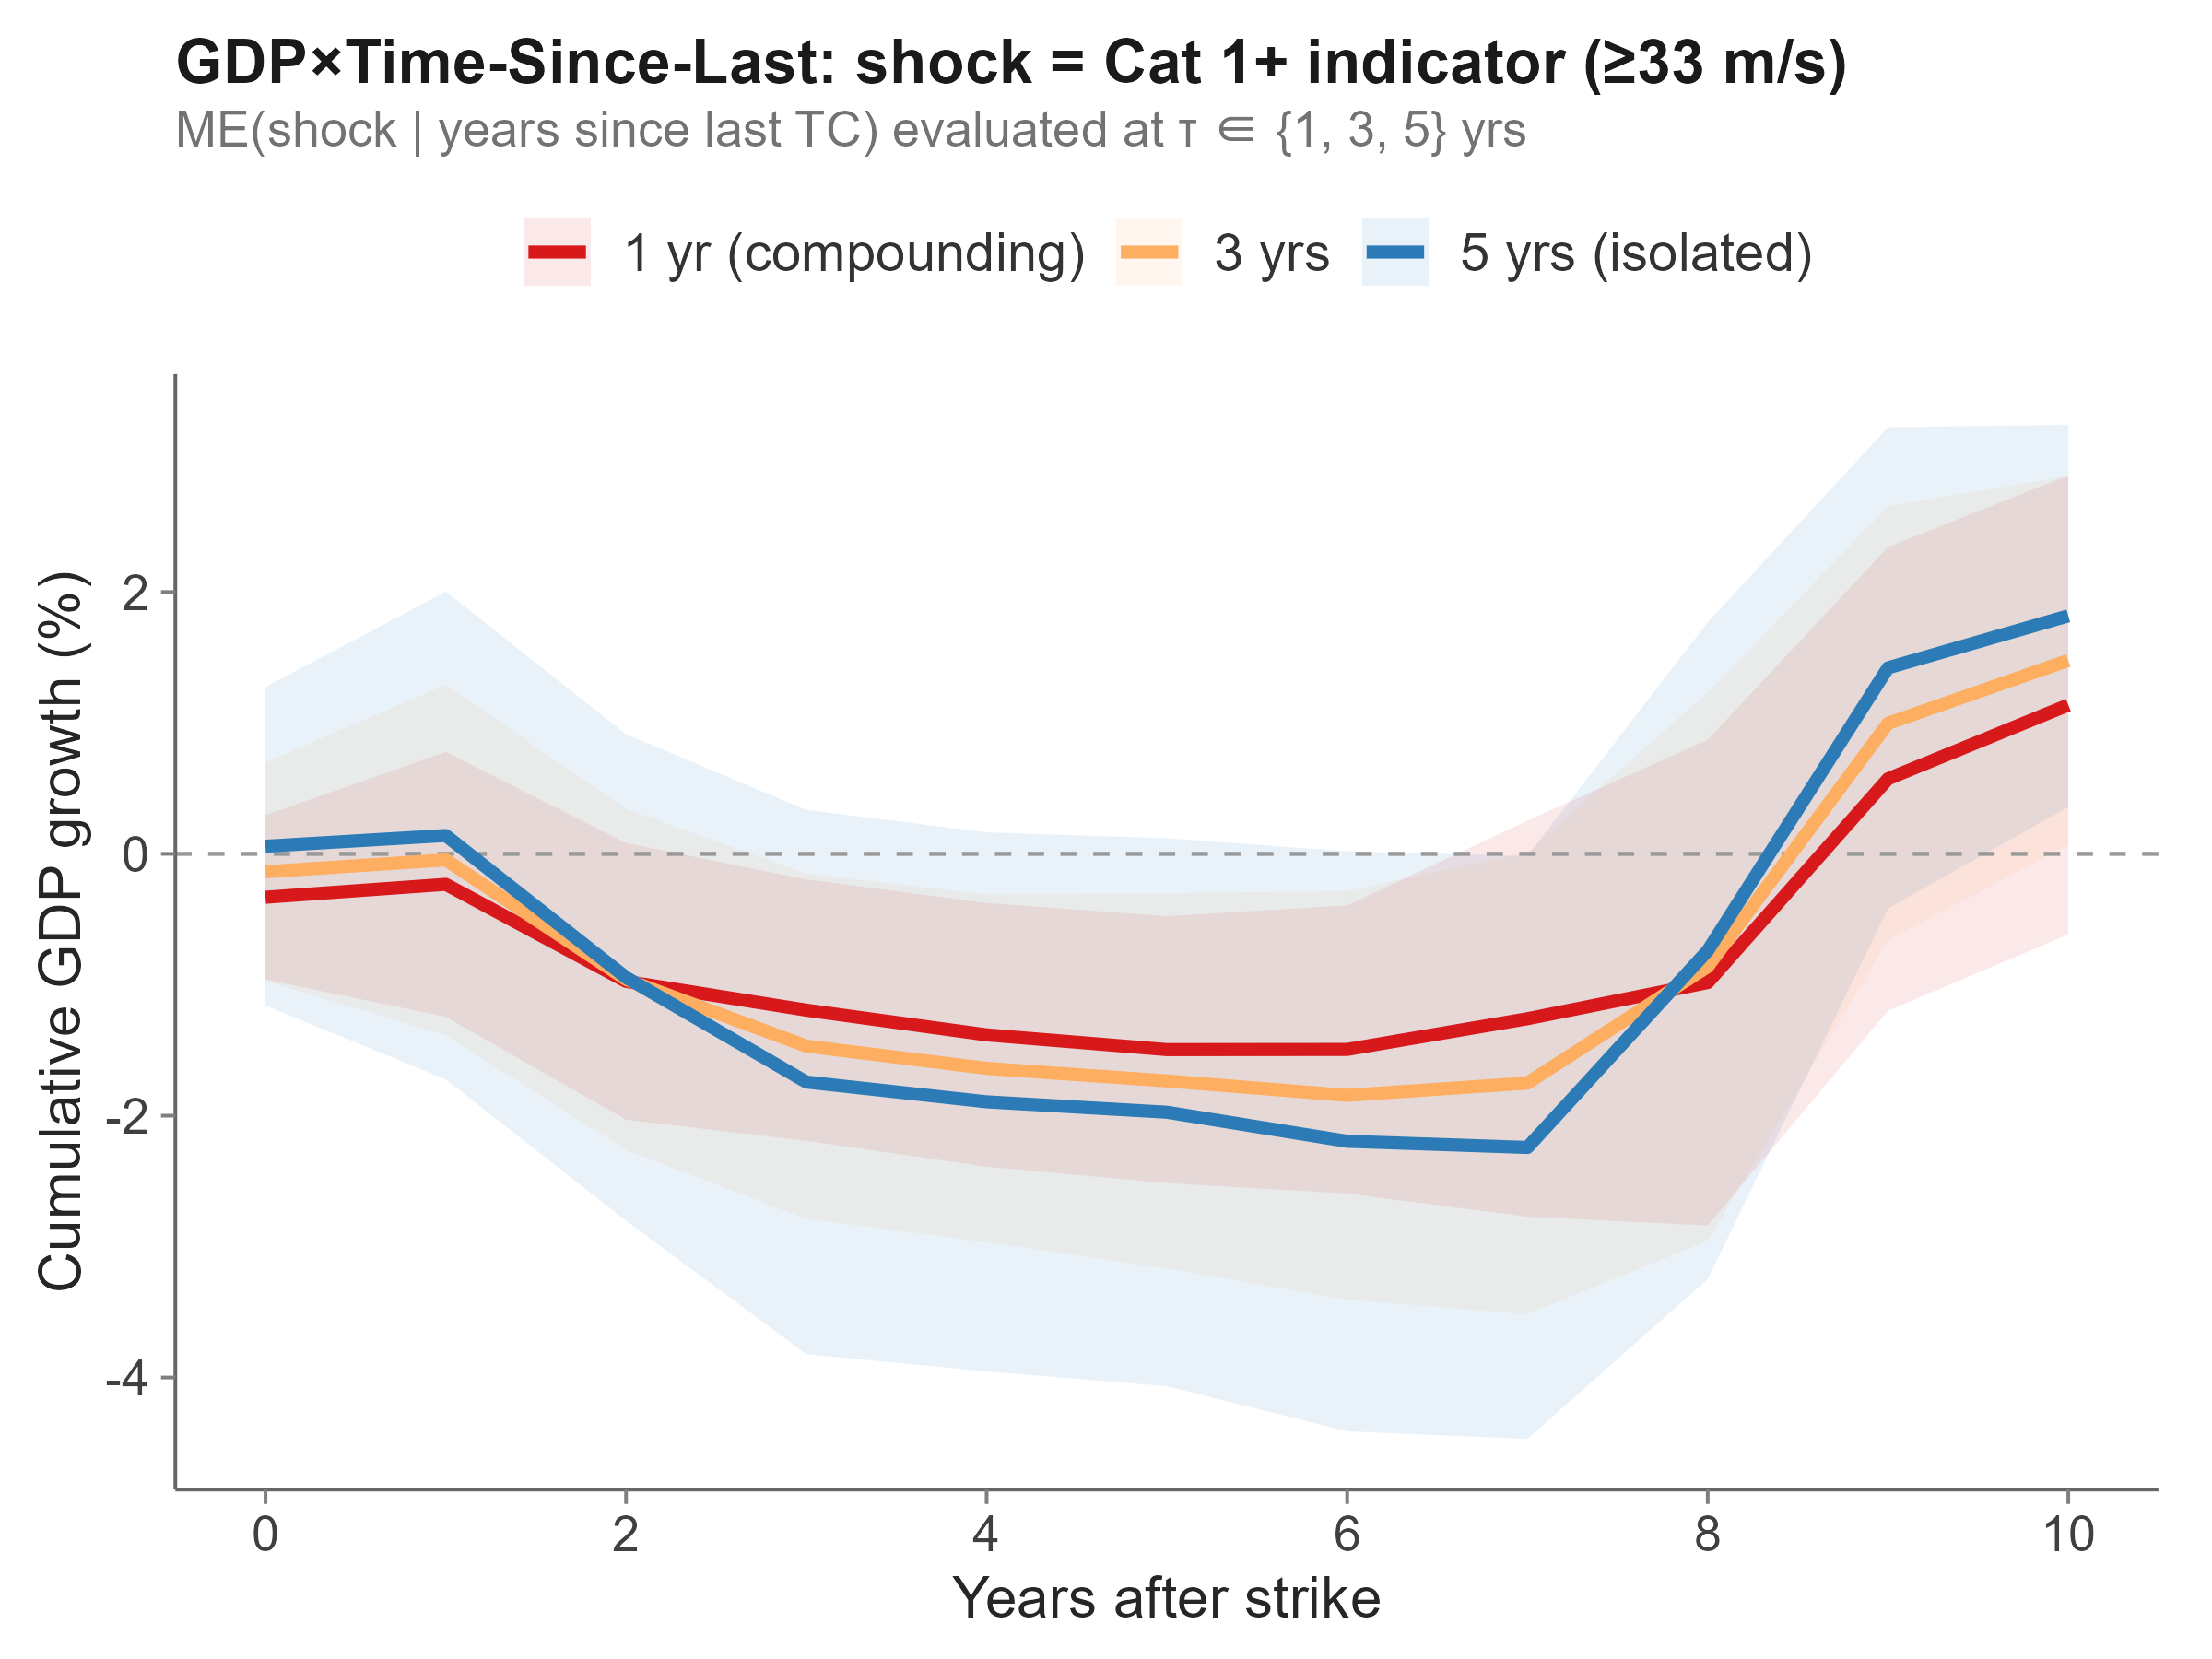
\includegraphics[width=0.82\textwidth,height=0.72\textheight,keepaspectratio]{figures/irf_compound_wind_cat1plus.png}

\smallskip\small
Shock = Cat\,1+ indicator ($\geq$33\,m/s).  Gradient is clear: isolated events
($\tau=5$, blue) generate larger GDP losses than compounding events ($\tau=1$, red).
\end{frame}

\begin{frame}{IRF: Cat\,2+ Binary $\times$ Time Since Last TC}
\centering
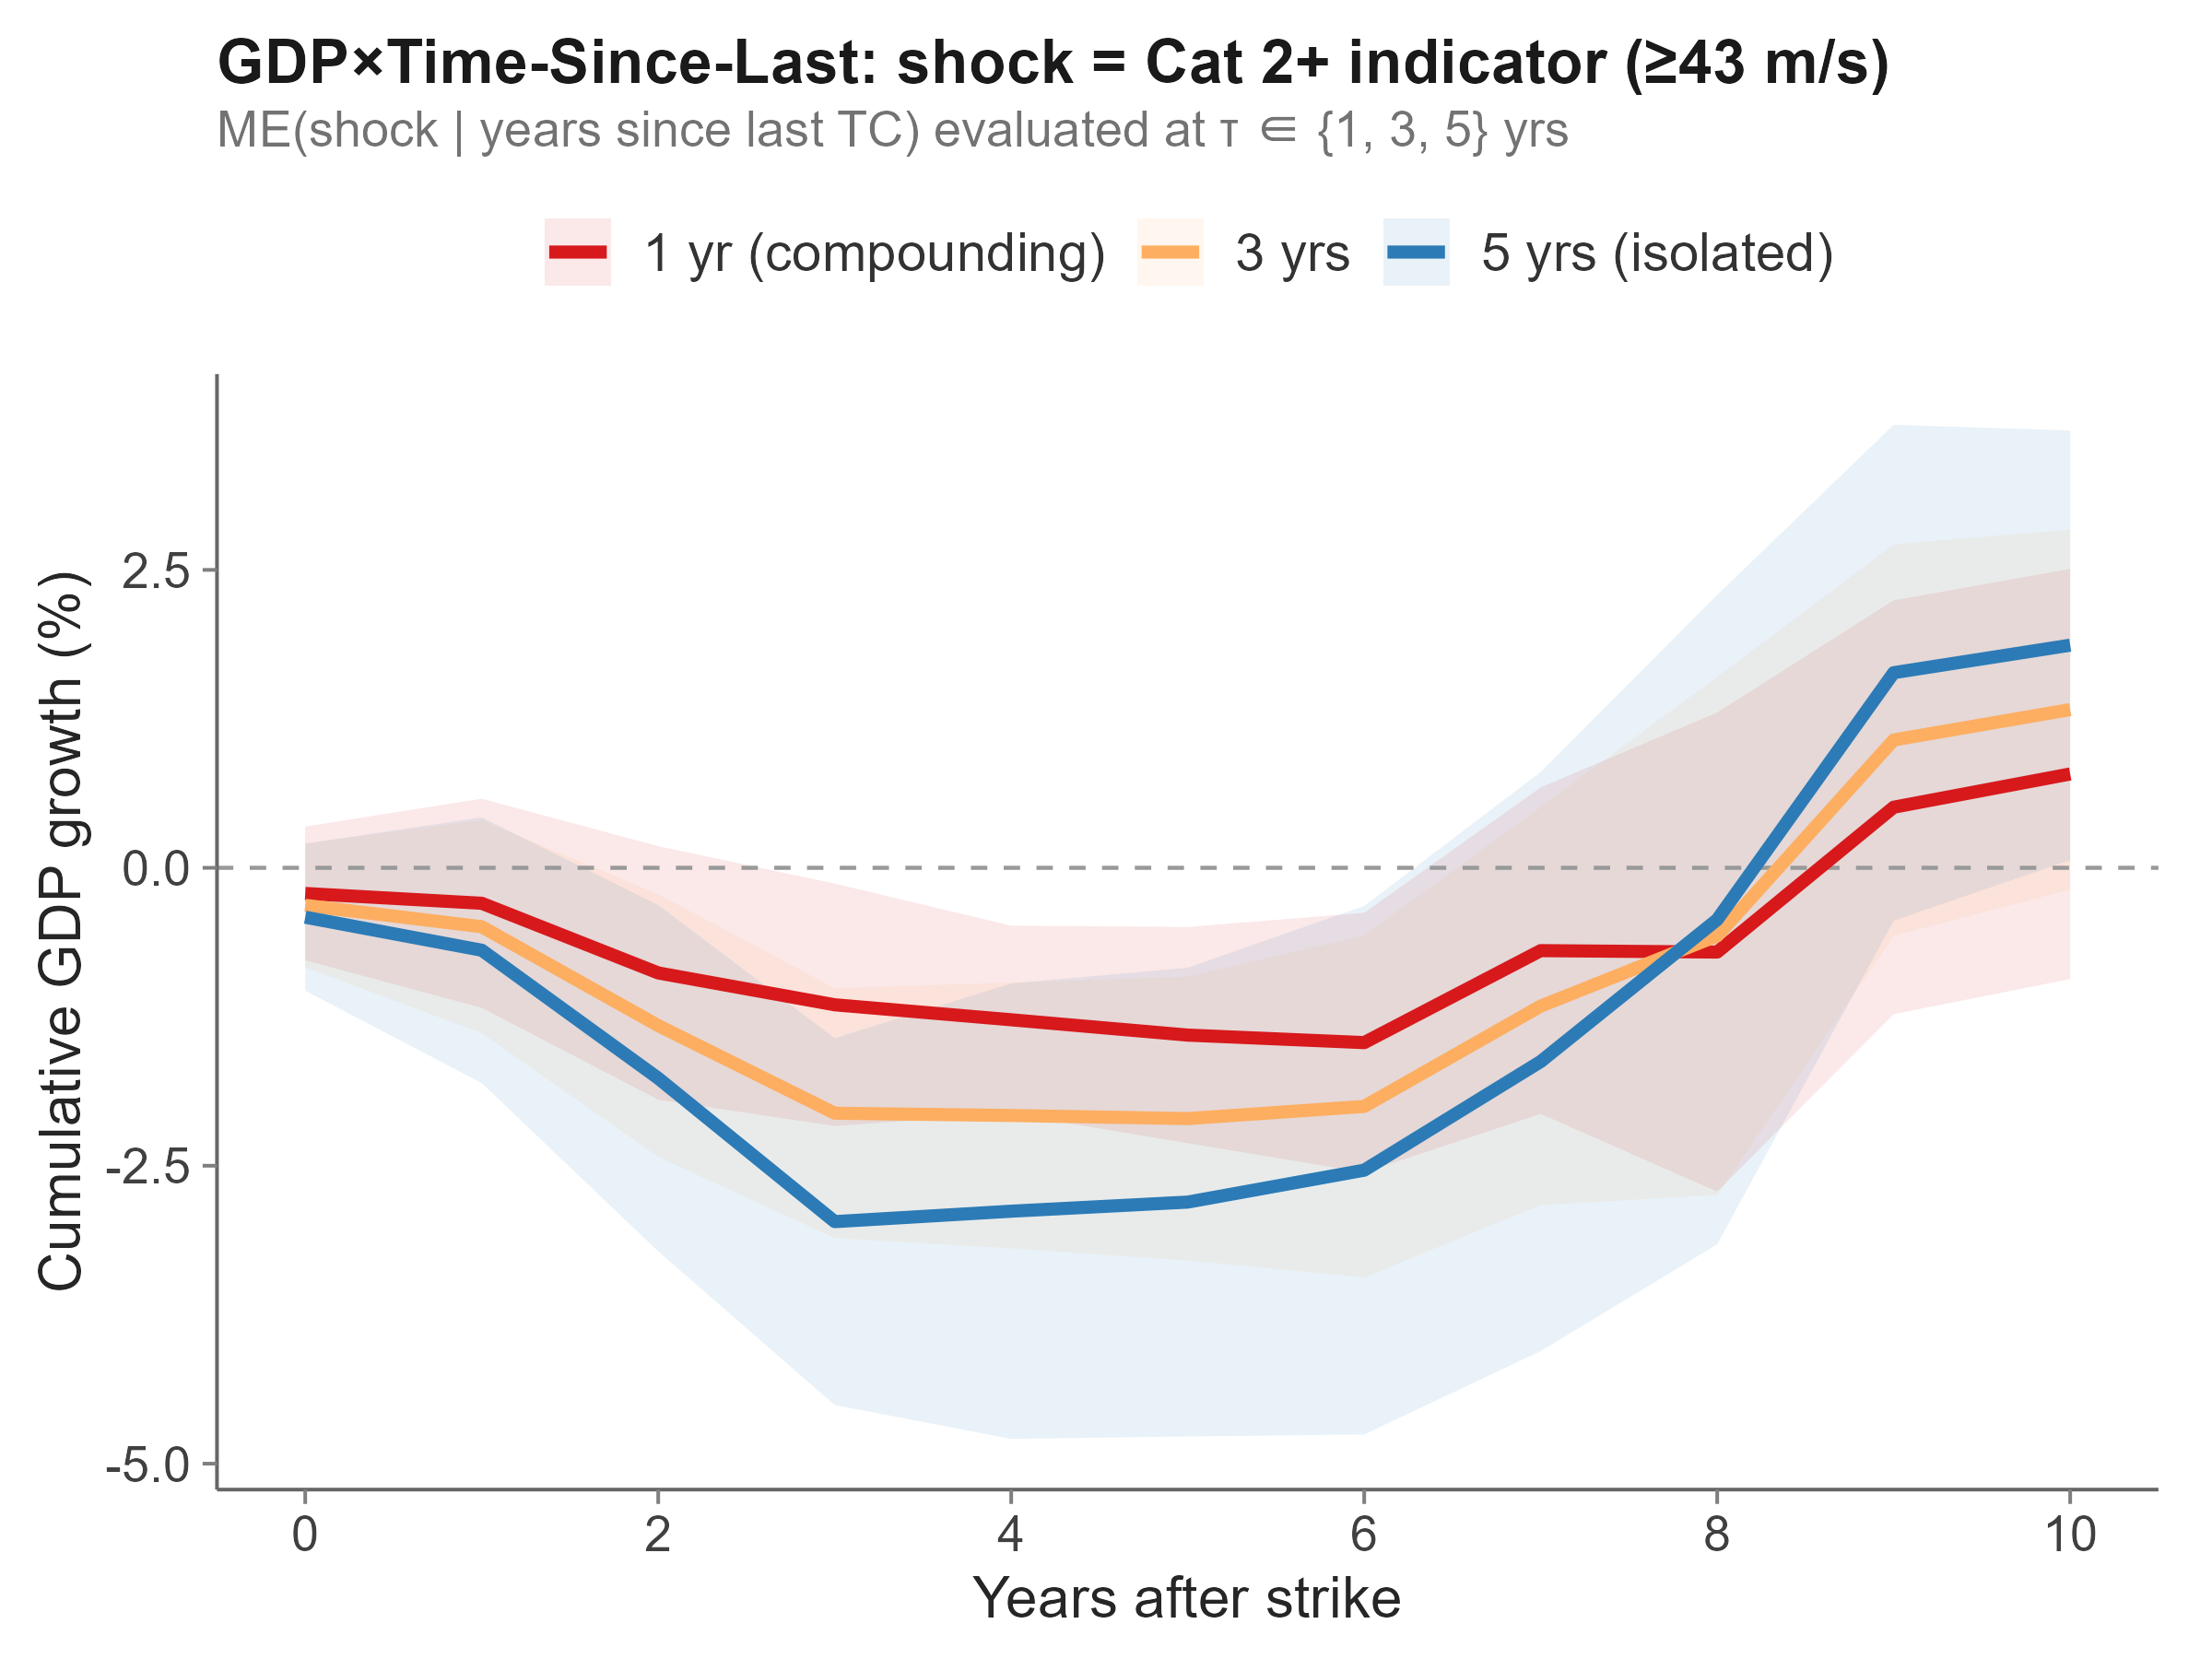
\includegraphics[width=0.82\textwidth,height=0.72\textheight,keepaspectratio]{figures/irf_compound_wind_cat2plus.png}

\smallskip\small
Shock = Cat\,2+ indicator ($\geq$43\,m/s).  The gradient sharpens: at $h=5$, the
isolated-minus-compounding gap is larger than for Cat\,1+, suggesting the
mechanism operates more strongly for intense events.
\end{frame}

\begin{frame}{IRF: Cat\,3+ Binary $\times$ Time Since Last TC}
\centering
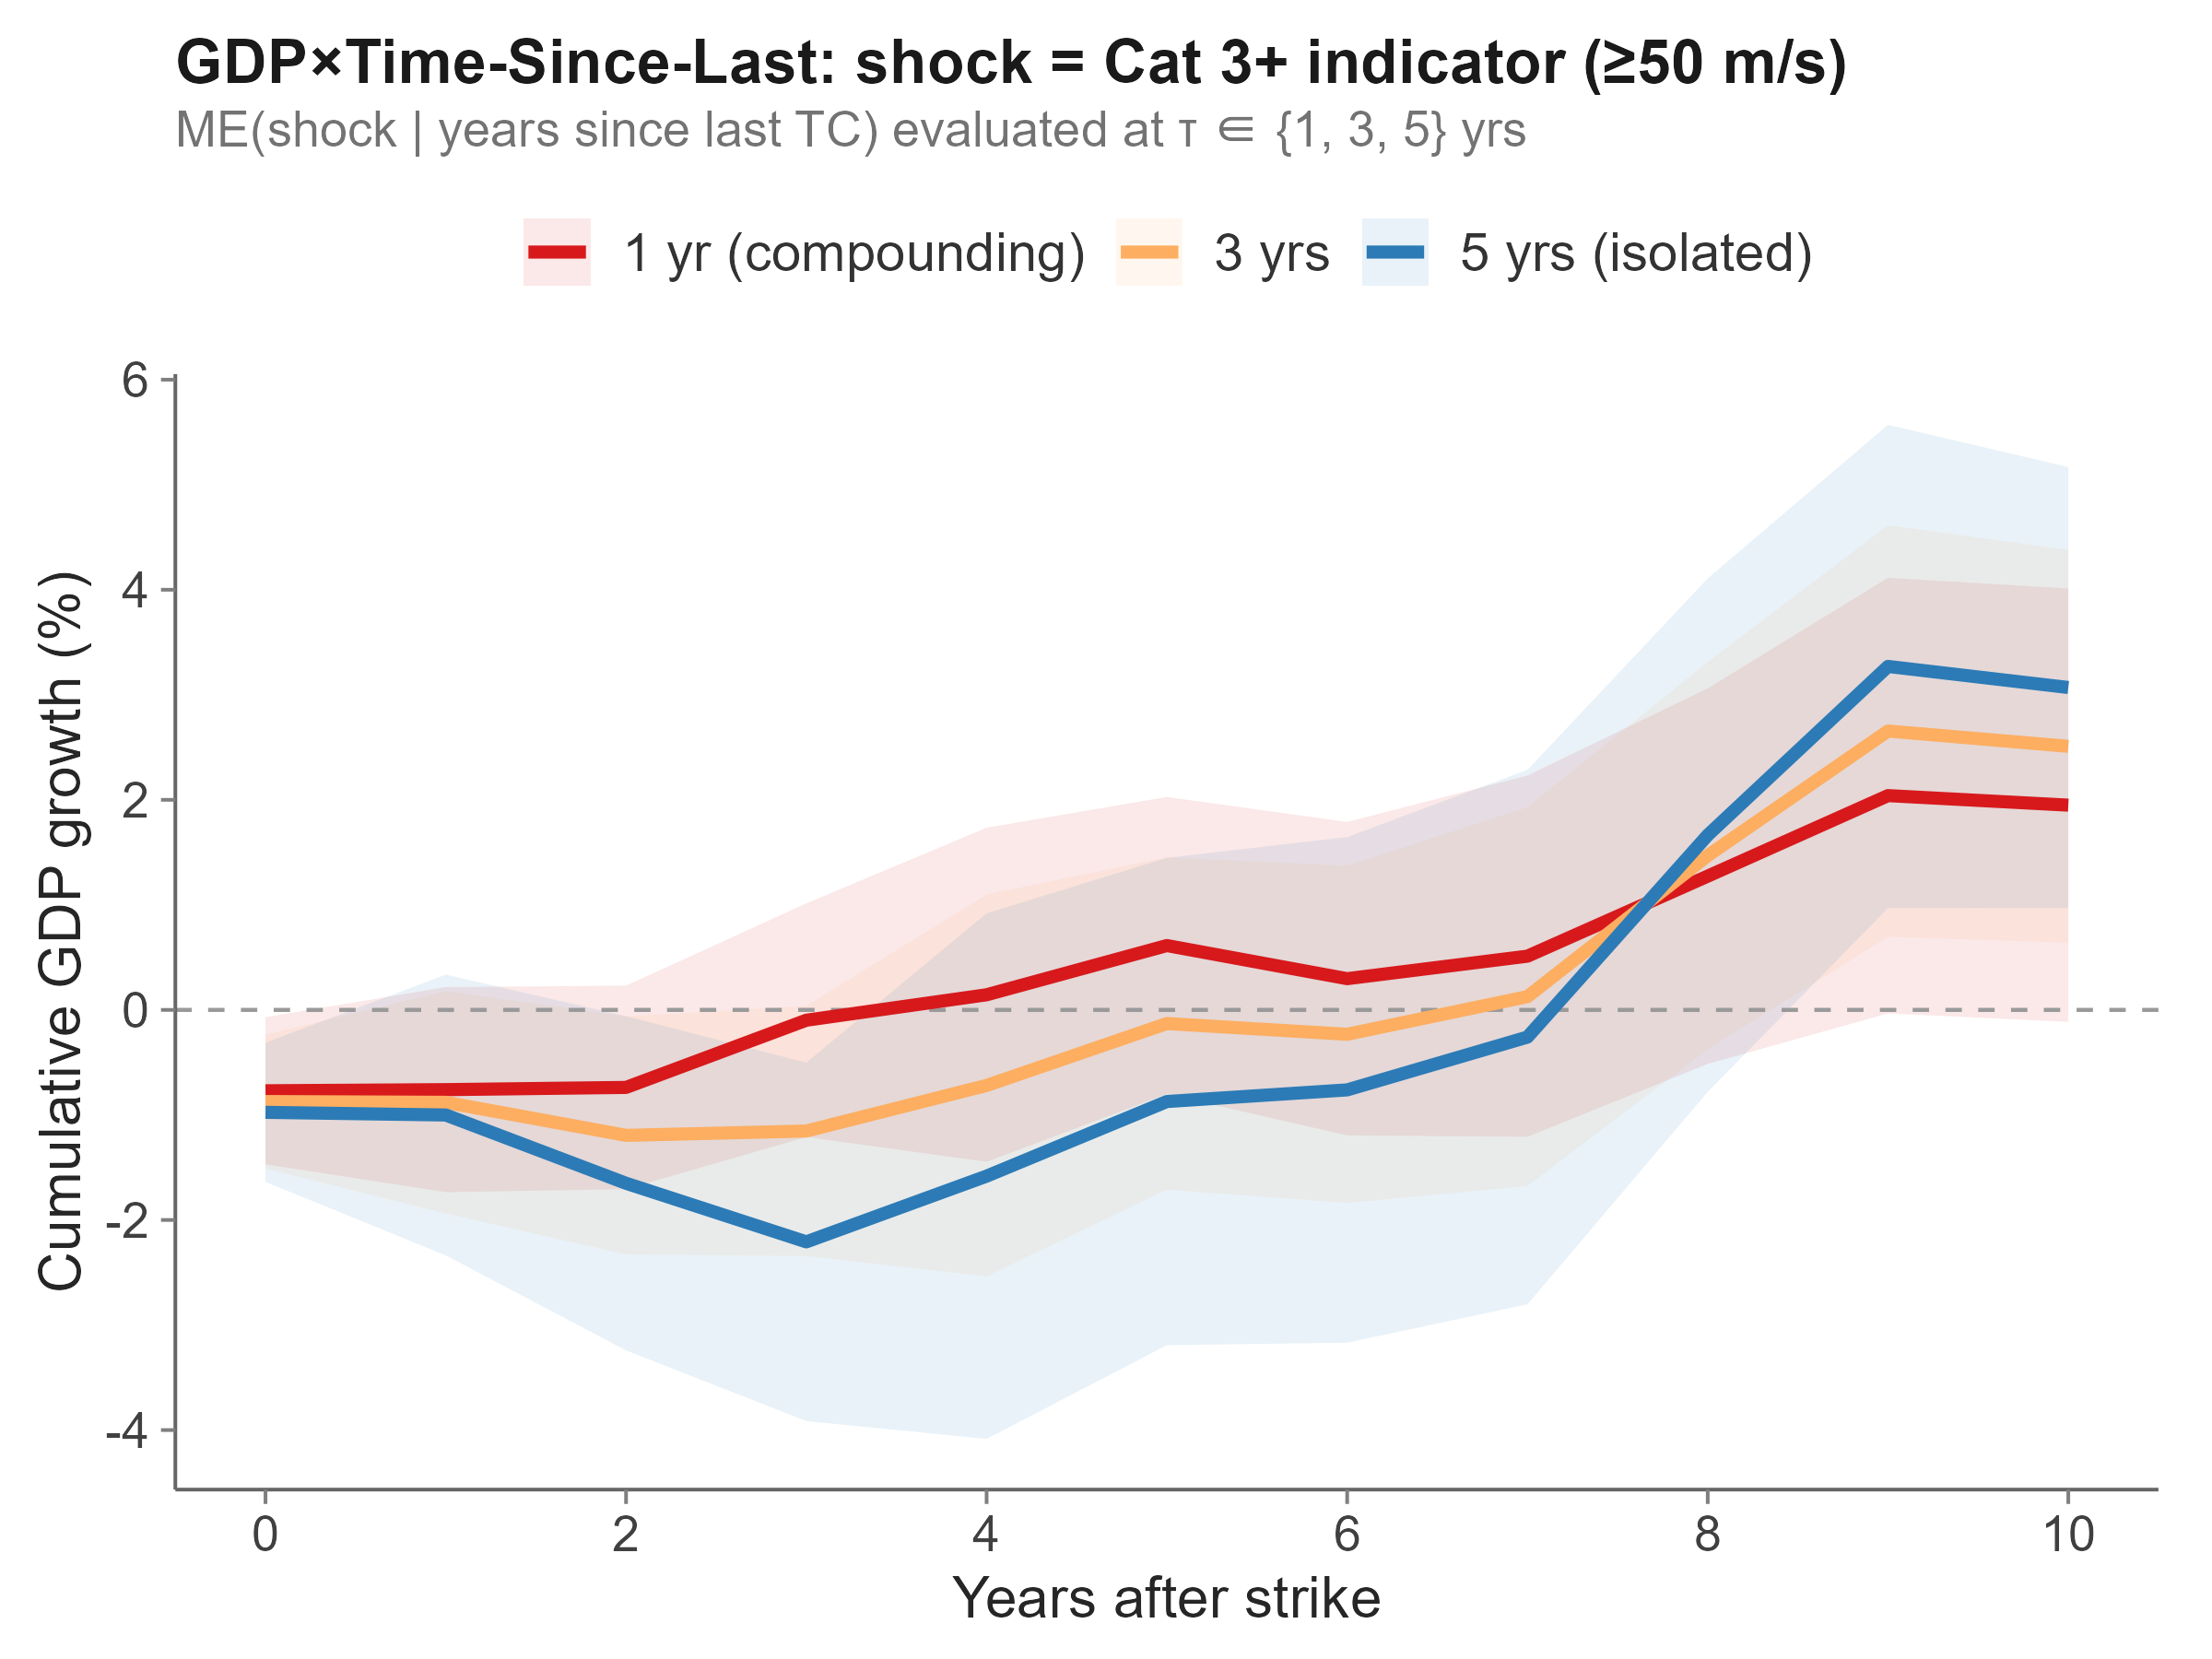
\includegraphics[width=0.82\textwidth,height=0.72\textheight,keepaspectratio]{figures/irf_compound_wind_cat3plus.png}

\smallskip\small
Shock = Cat\,3+ indicator ($\geq$50\,m/s).  Fewer treated observations; wider
confidence bands.  Back-to-back major events ($\tau=1$) show attenuated GDP
cost --- consistent with reduced destructible stock after a prior major event.
\end{frame}

% ===============================================================
\section{Robustness: Probing the $\bar{W}$ Confound}
% ===============================================================
{\hideframenumber\begin{frame}\sectionpage\end{frame}\showframenumber}

\begin{frame}{Strategy: Three Tests for $\bar{W}$ Confounding}

The gradient (isolated $>$ compounding GDP loss) could reflect:

\medskip
\begin{enumerate}
  \item \textbf{Dilution by never-struck controls:} never-struck countries
        have $\tau = \texttt{NA}$ and are dropped from the compound LP, but
        their presence in the full panel may affect estimates.
        \textit{Fix:} restrict to ever-treated countries ($\bar{W}_i>0$).

  \medskip
  \item \textbf{Geographic concentration:} compound events cluster in specific
        regions (East/Southeast Asia, Caribbean) with distinct recovery
        patterns.  \textit{Fix:} leave-one-continent-out (LOCO).

  \medskip
  \item \textbf{$\bar{W}$ composition:} the gradient is entirely explained by
        comparing high-$\bar{W}$ countries (short $\tau$) to low-$\bar{W}$
        countries (long $\tau$).  \textit{Fix:} estimate the gradient
        \emph{within} high- and low-climatology groups separately.
        If it vanishes within groups, $\tau$ has no independent variation.
\end{enumerate}

\medskip\small
\textbf{Spoiler:} Test~3 fails for a data reason --- $\tau$ has essentially
\emph{no variation} within the High-$\bar{W}$ group (98\,\% of obs have
$\tau\leq2$).  And the residualised-$\tau$ LP (Test~4 below) shows the
gradient disappears once the $\bar{W}$--$\tau$ correlation is removed.
\normalsize
\end{frame}

\begin{frame}{Diagnostic: $\tau$ Has Almost No Variation in High-$\bar{W}$ Countries}
\centering
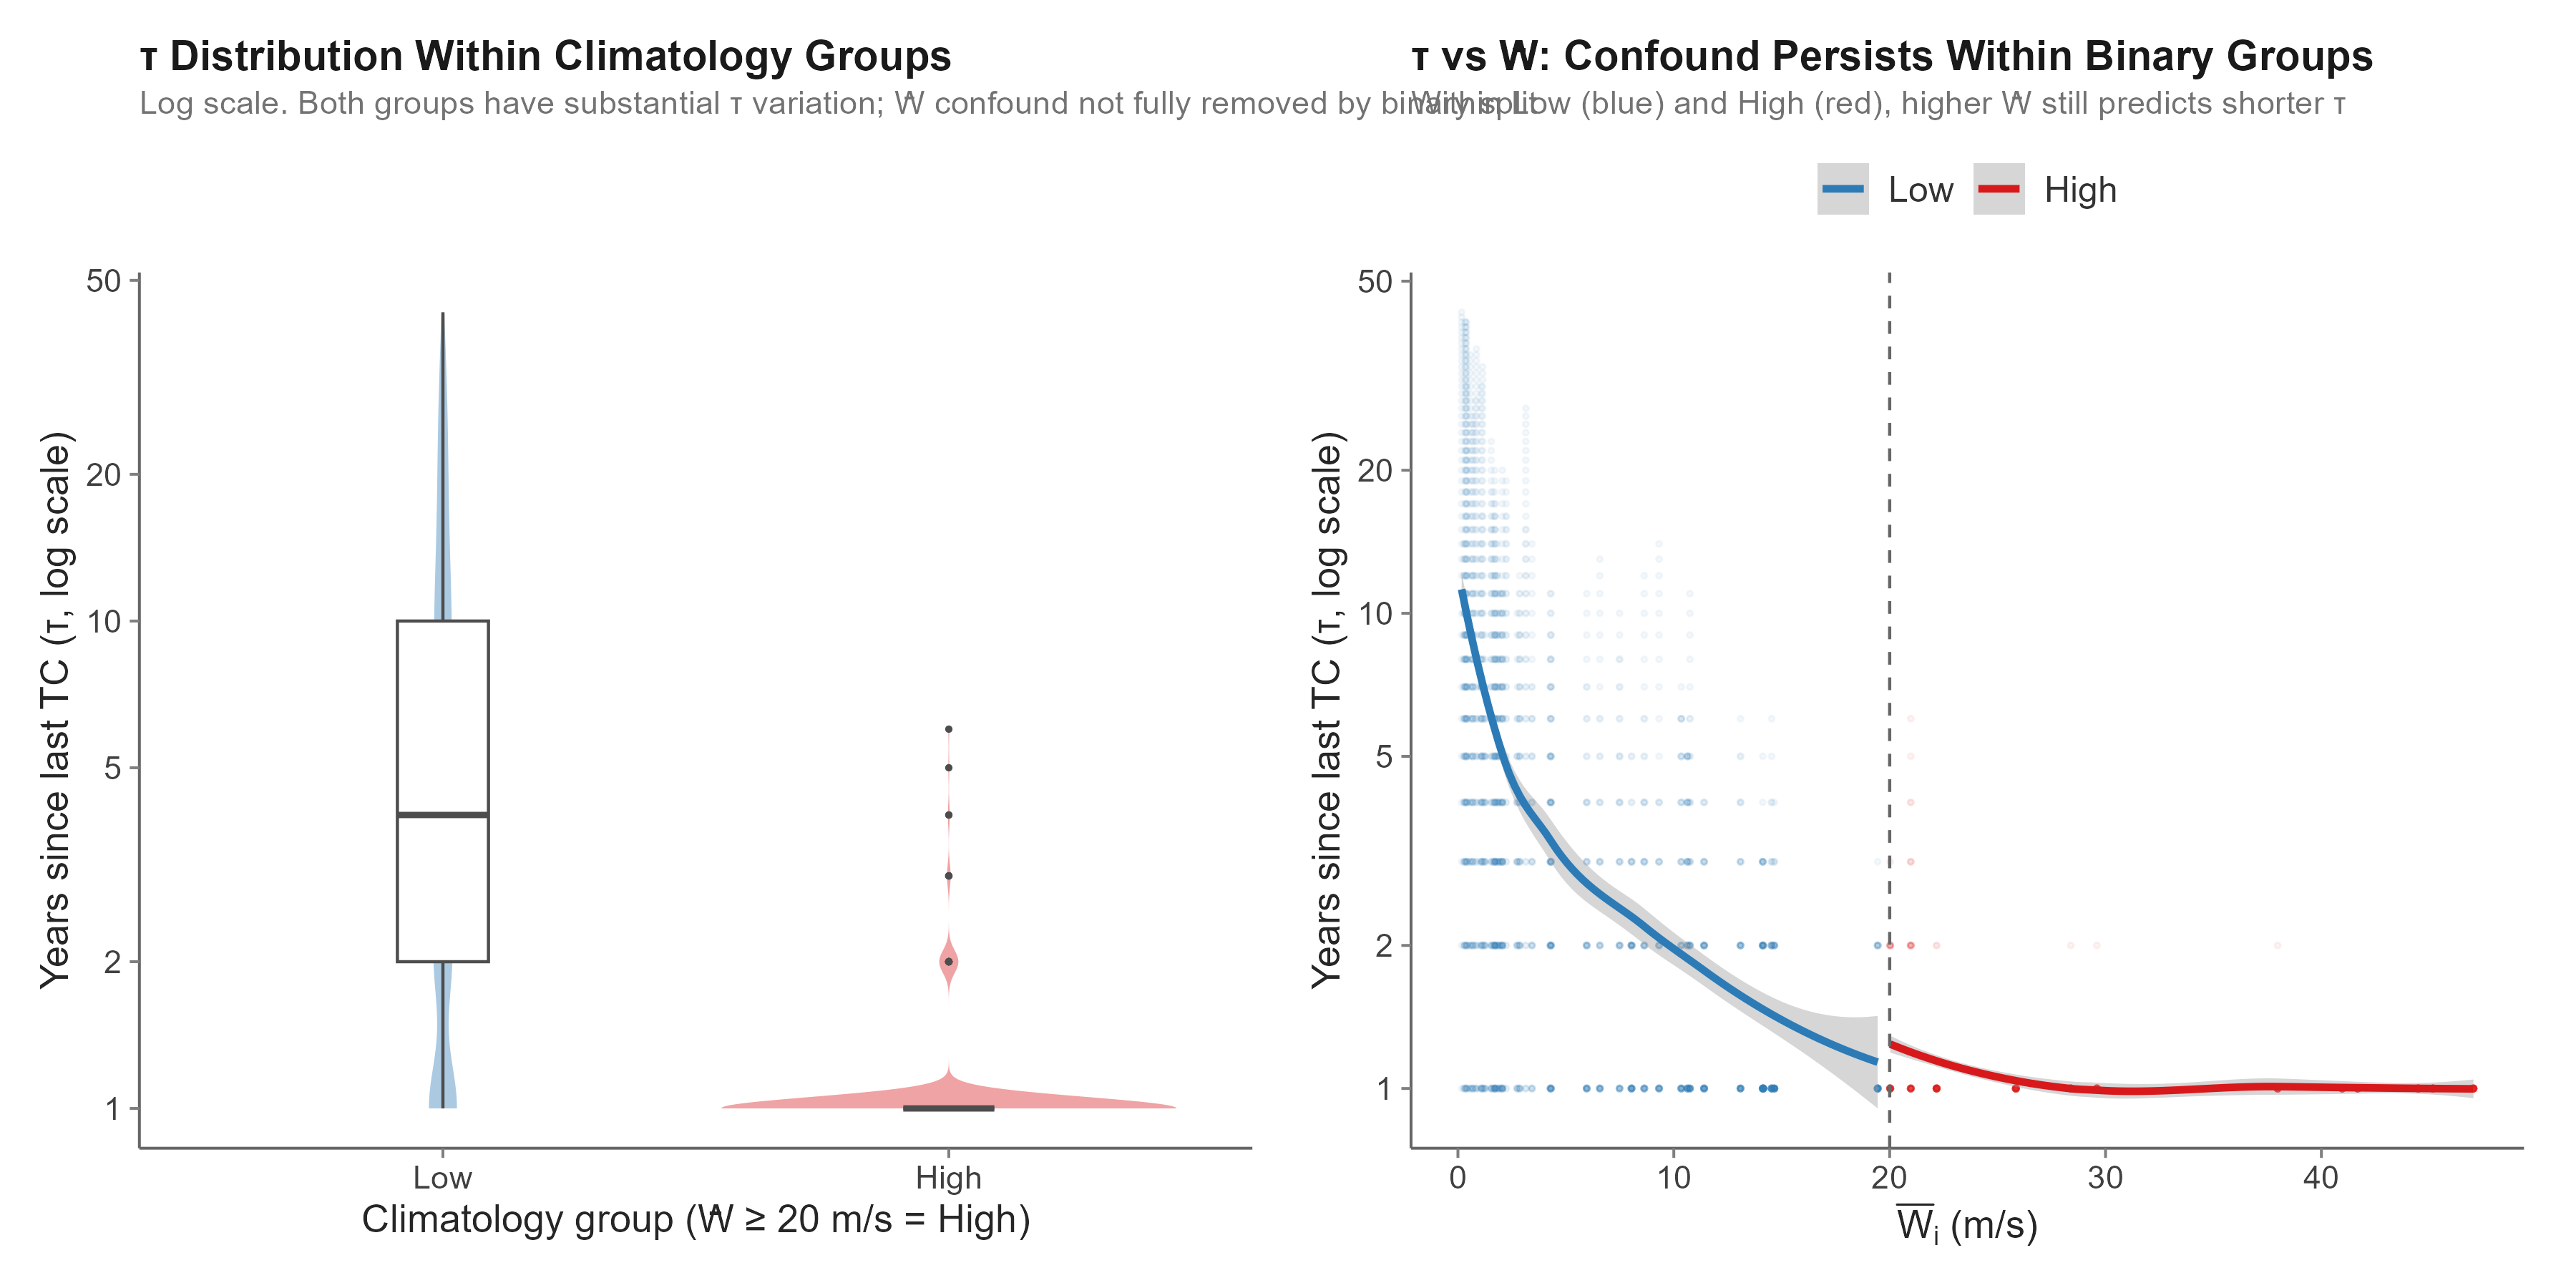
\includegraphics[width=0.96\textwidth,height=0.68\textheight,keepaspectratio]{figures/compound_rob_tau_diagnostic.png}

\smallskip\small
\textbf{Left:} $\tau$ distribution (log scale) within binary $\bar{W}$ groups.
\textbf{Right:} within each group, higher $\bar{W}$ still predicts shorter $\tau$ (LOESS).
\textbf{Key fact:} in the High group ($\bar{W}\geq20$), 98.5\,\% of obs have
$\tau\leq2$ yrs --- effectively \emph{no variation} in $\tau$.
Any ``gradient'' estimated within High is extrapolation, not identification.
\end{frame}

\begin{frame}{Full Sample vs Ever-Treated}
\centering
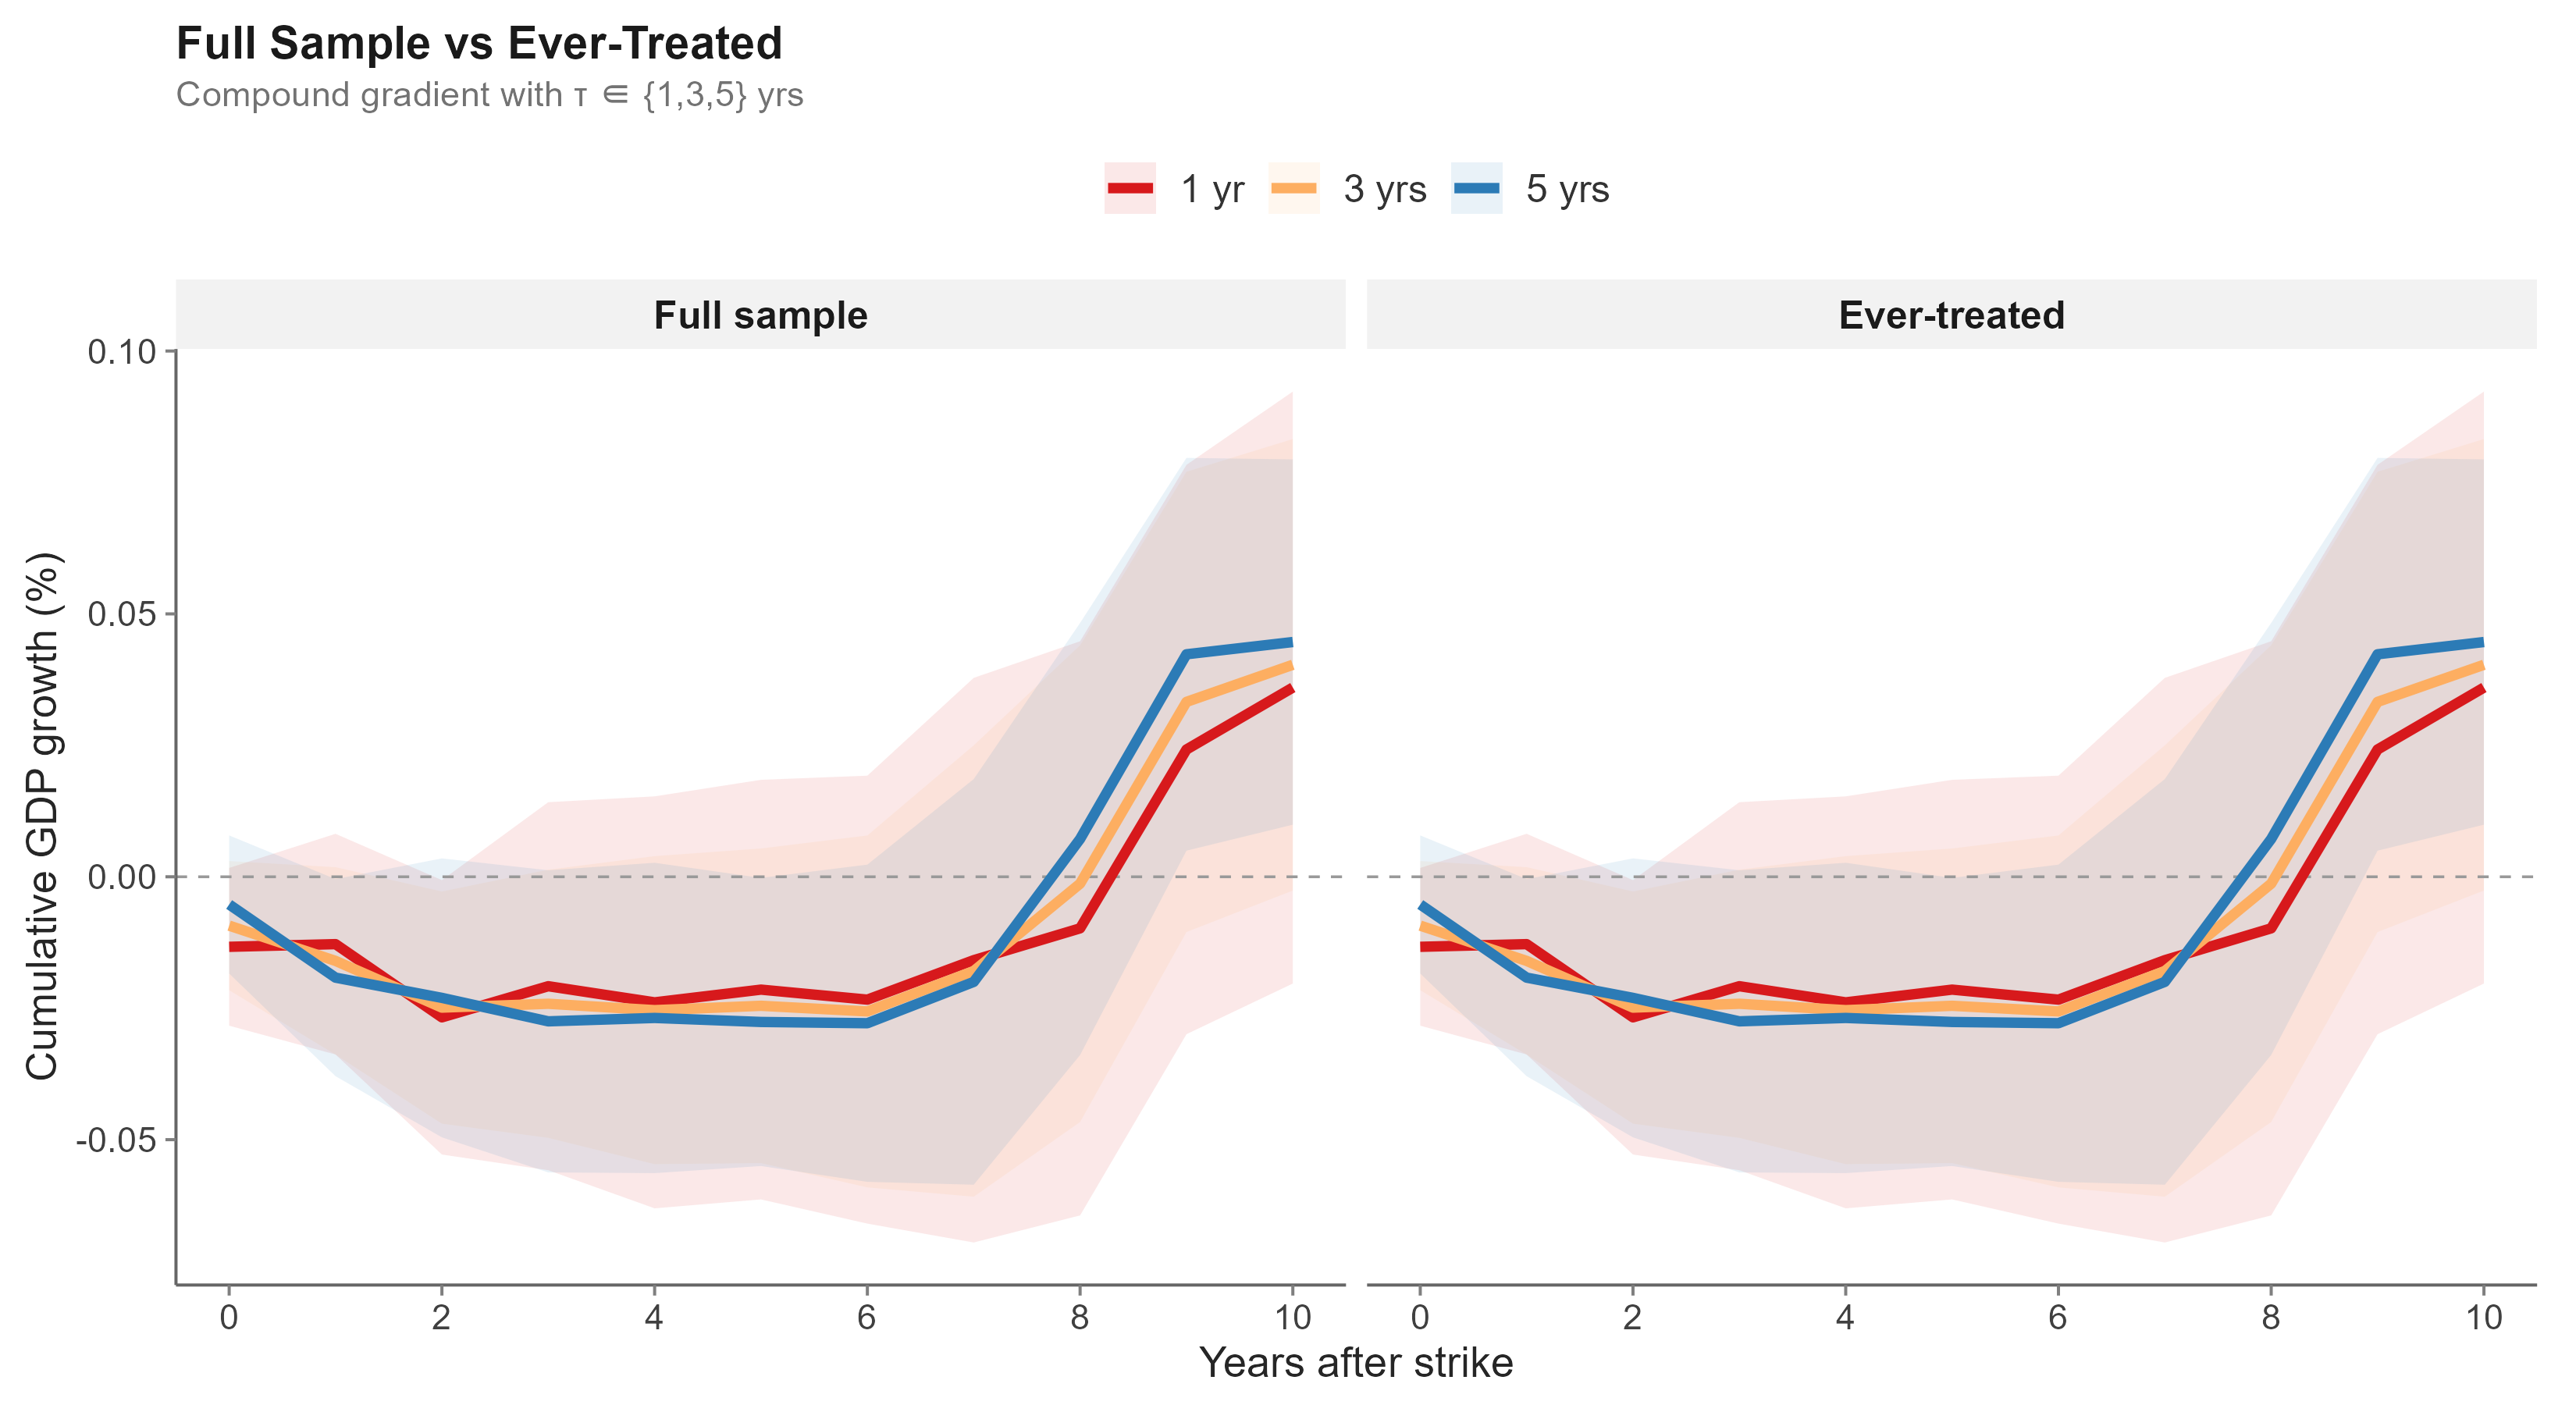
\includegraphics[width=0.96\textwidth,height=0.72\textheight,keepaspectratio]{figures/compound_rob_samples.png}

\smallskip\small
Left: full panel.  Right: ever-struck countries only ($\bar{W}_i>0$).
Gradient is similar in both samples --- not driven by never-struck controls.
\end{frame}

\begin{frame}{Leave-One-Continent-Out}
\centering
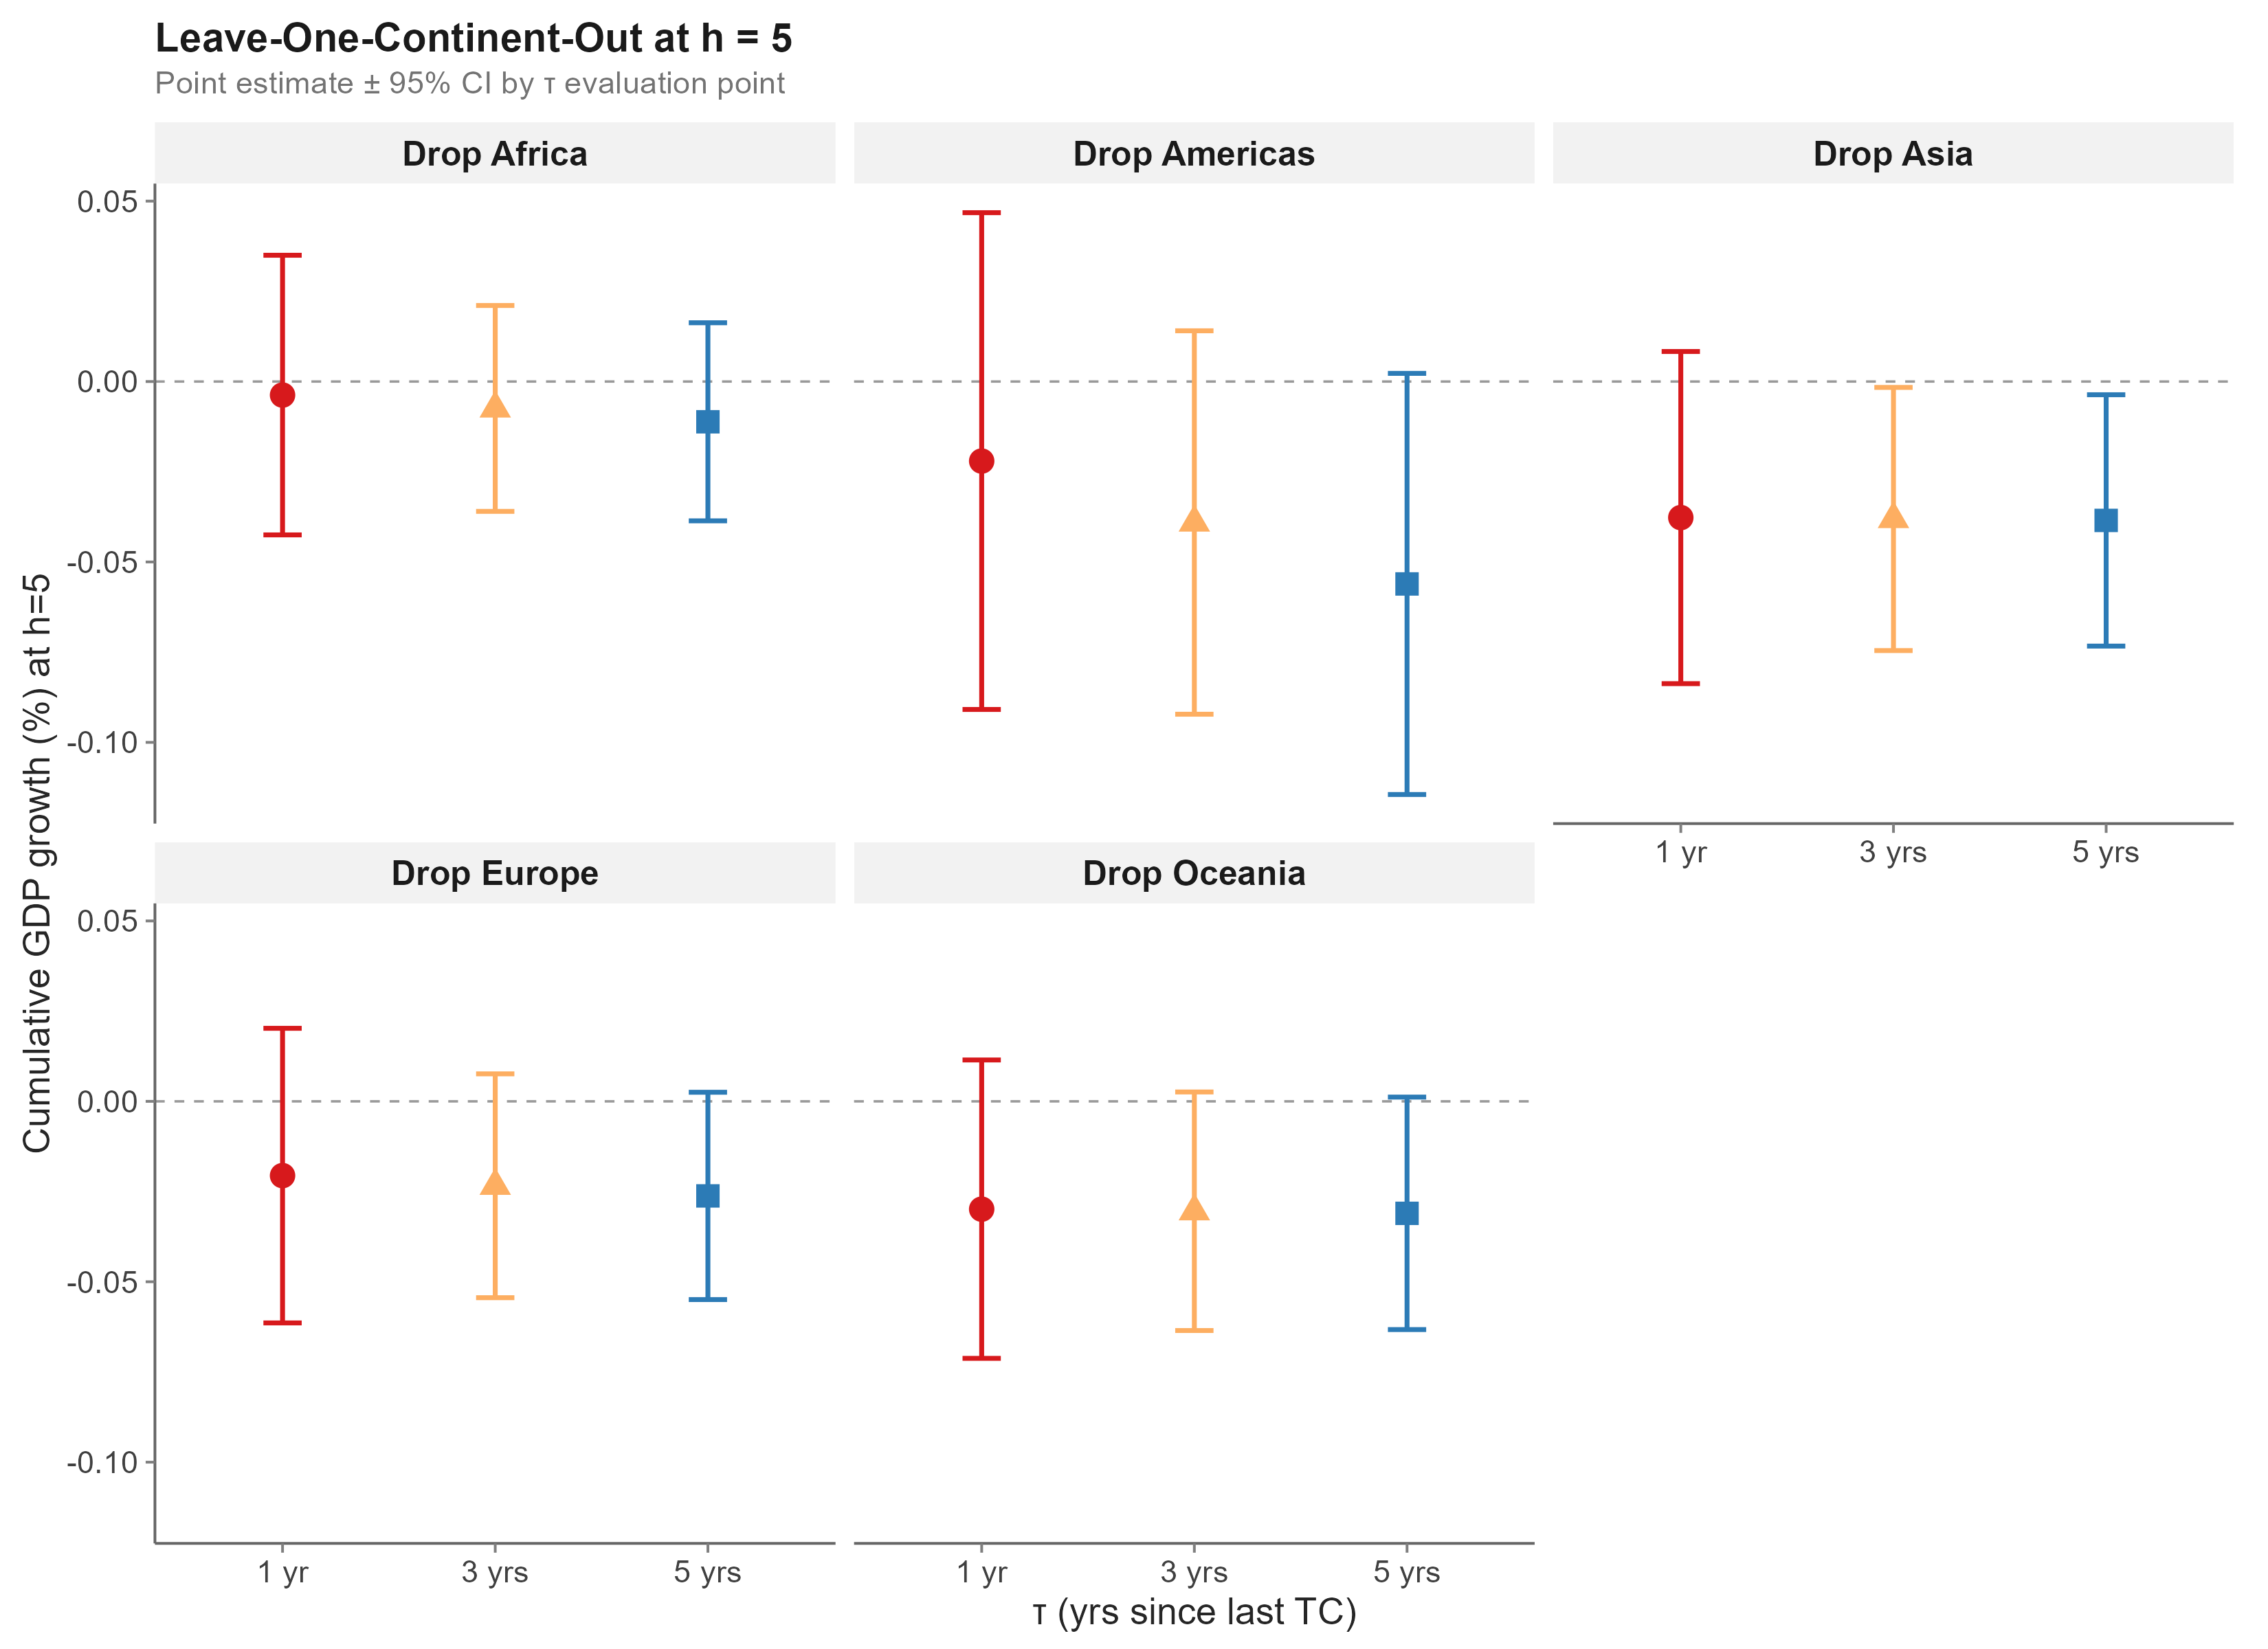
\includegraphics[width=0.96\textwidth,height=0.72\textheight,keepaspectratio]{figures/compound_rob_loco.png}

\smallskip\small
Maxwind-resid IRF at $h=5$, dropping one continent at a time.
No single region drives the pattern.
\end{frame}

\begin{frame}{Within Binary and Tercile $\bar{W}$ Groups}
\centering
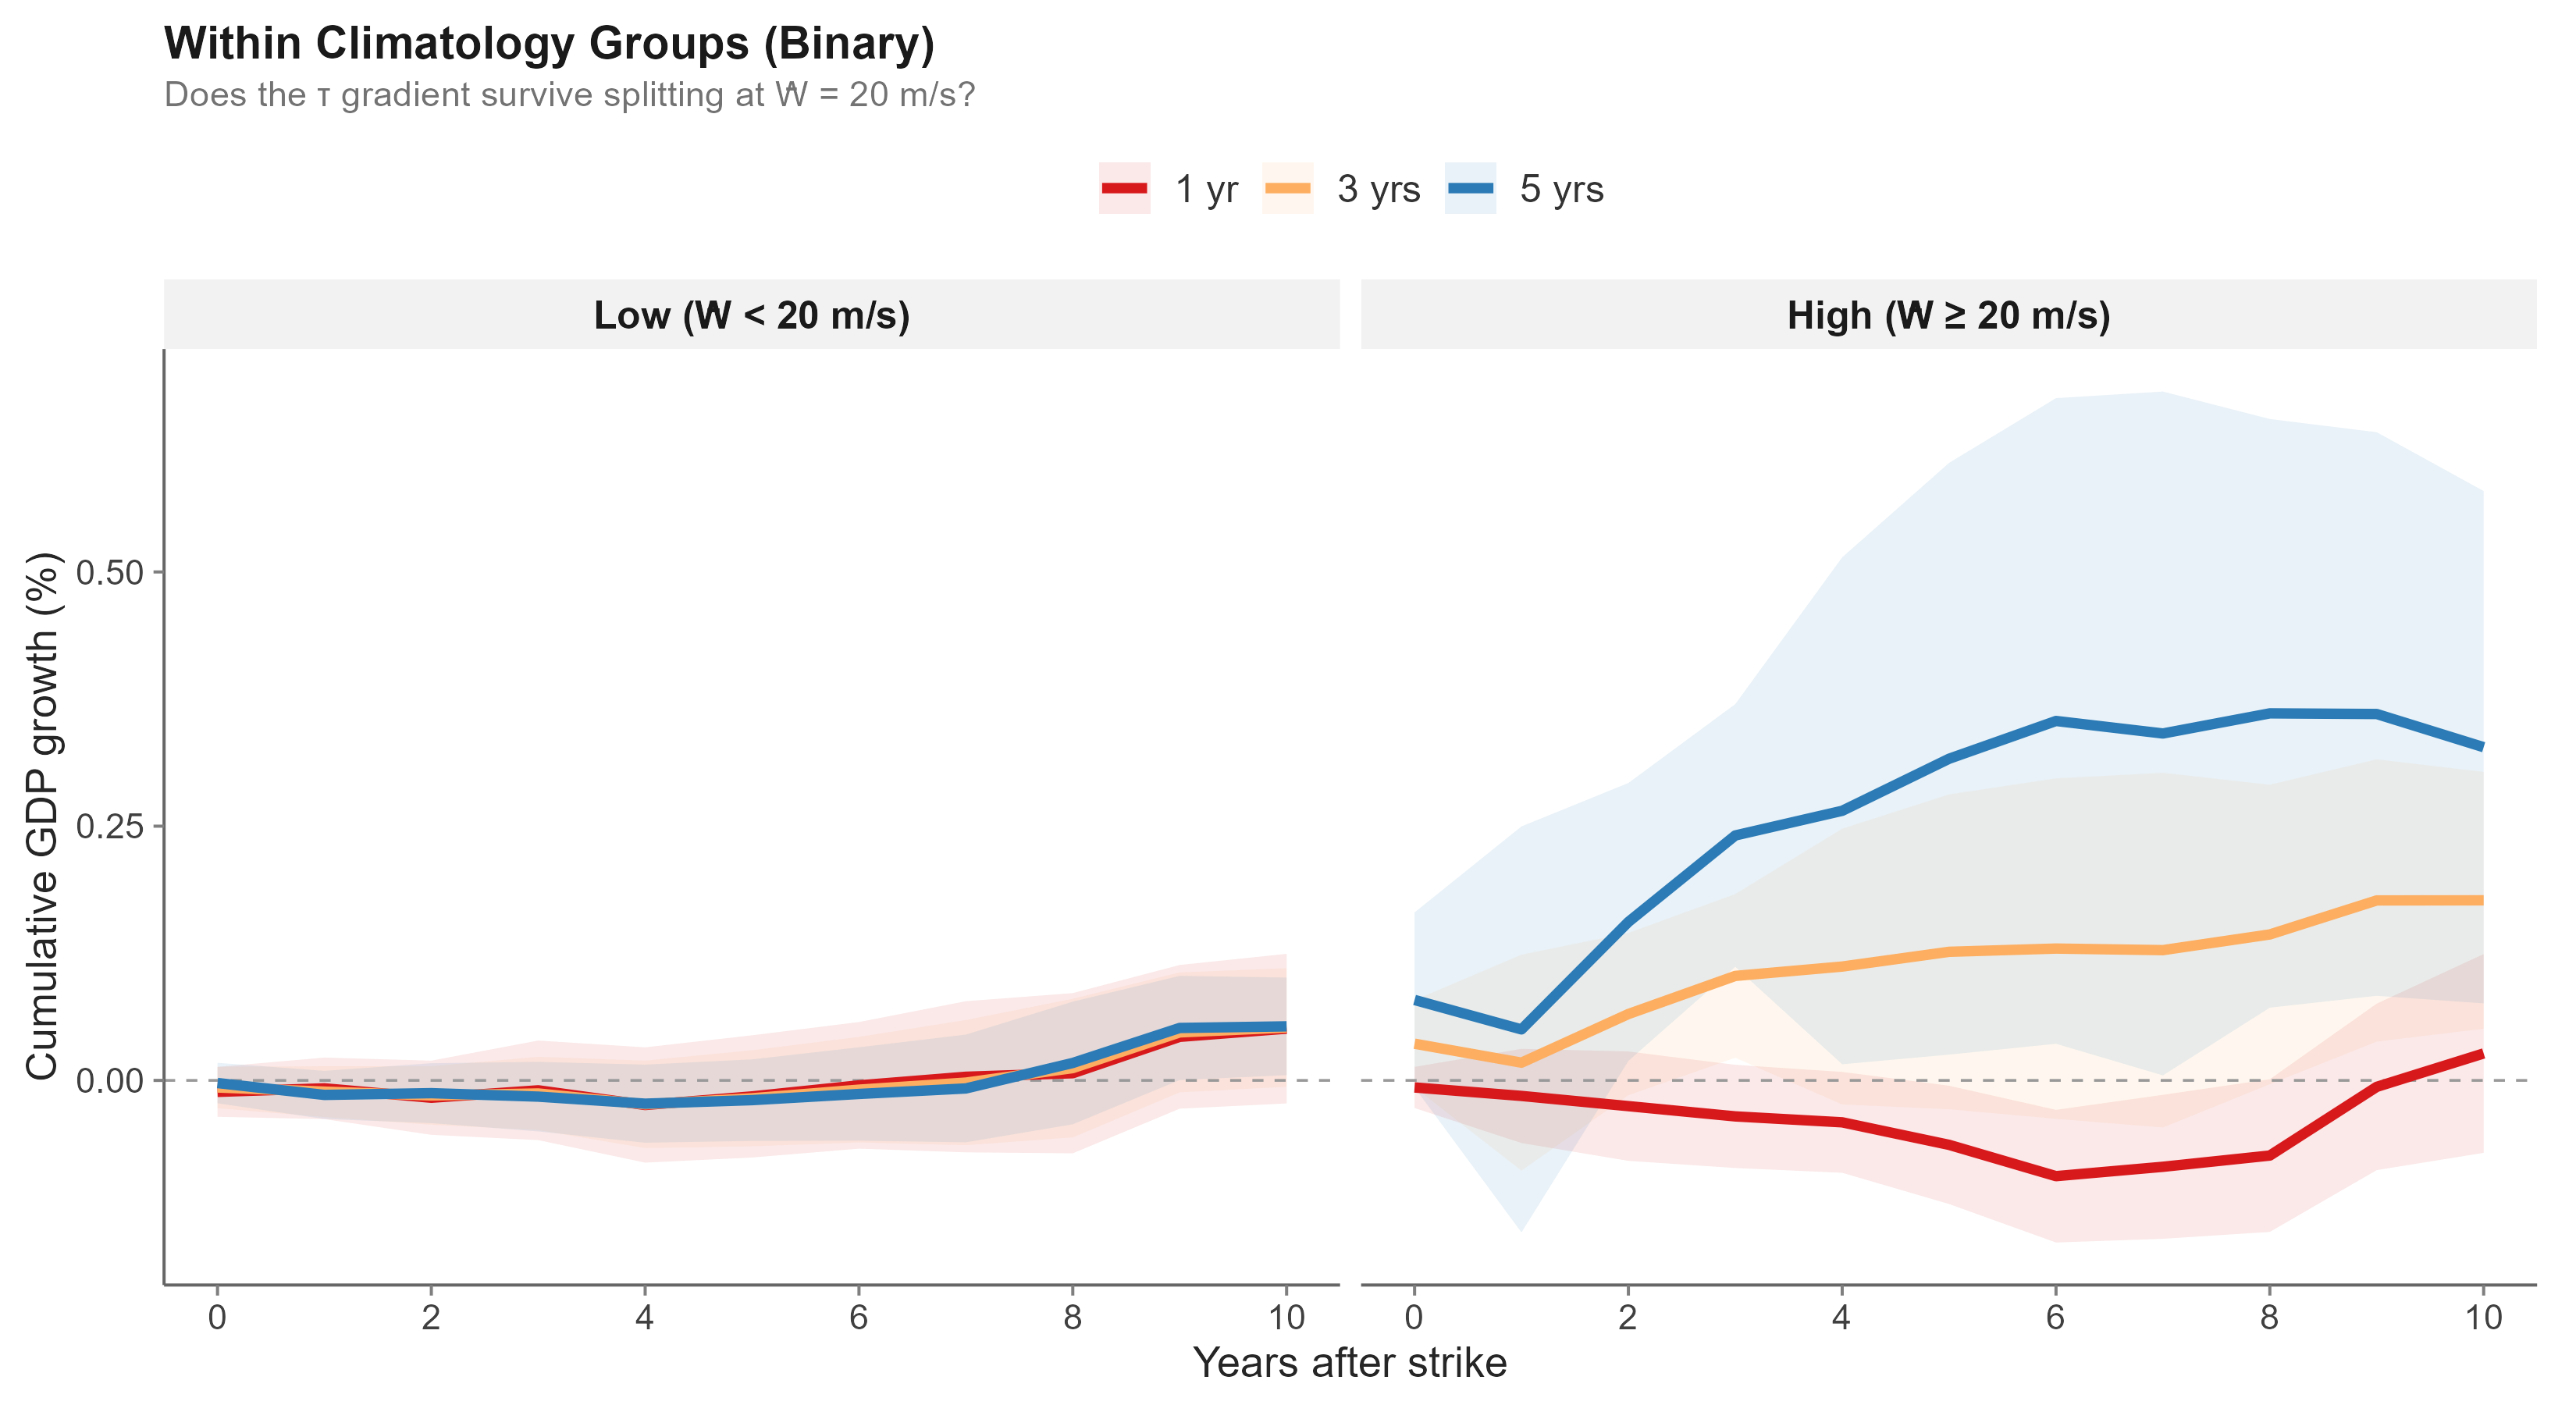
\includegraphics[width=0.96\textwidth,height=0.68\textheight,keepaspectratio]{figures/compound_rob_clim_groups.png}

\smallskip\small
Binary split at $\bar{W}=20$\,m/s.  In the \textbf{Low} group (blue), the gradient
is flat --- $\tau=1,3,5$ lines overlap.
In the \textbf{High} group (red), a large apparent gradient emerges, but this is
an artefact: 98.5\,\% of High-group obs have $\tau\leq2$, so the LP
extrapolates to $\tau=5$ with virtually no support.
\end{frame}

\begin{frame}{Within $\bar{W}$ Groups (Fixed Breaks: 10 and 30\,m/s)}
\centering
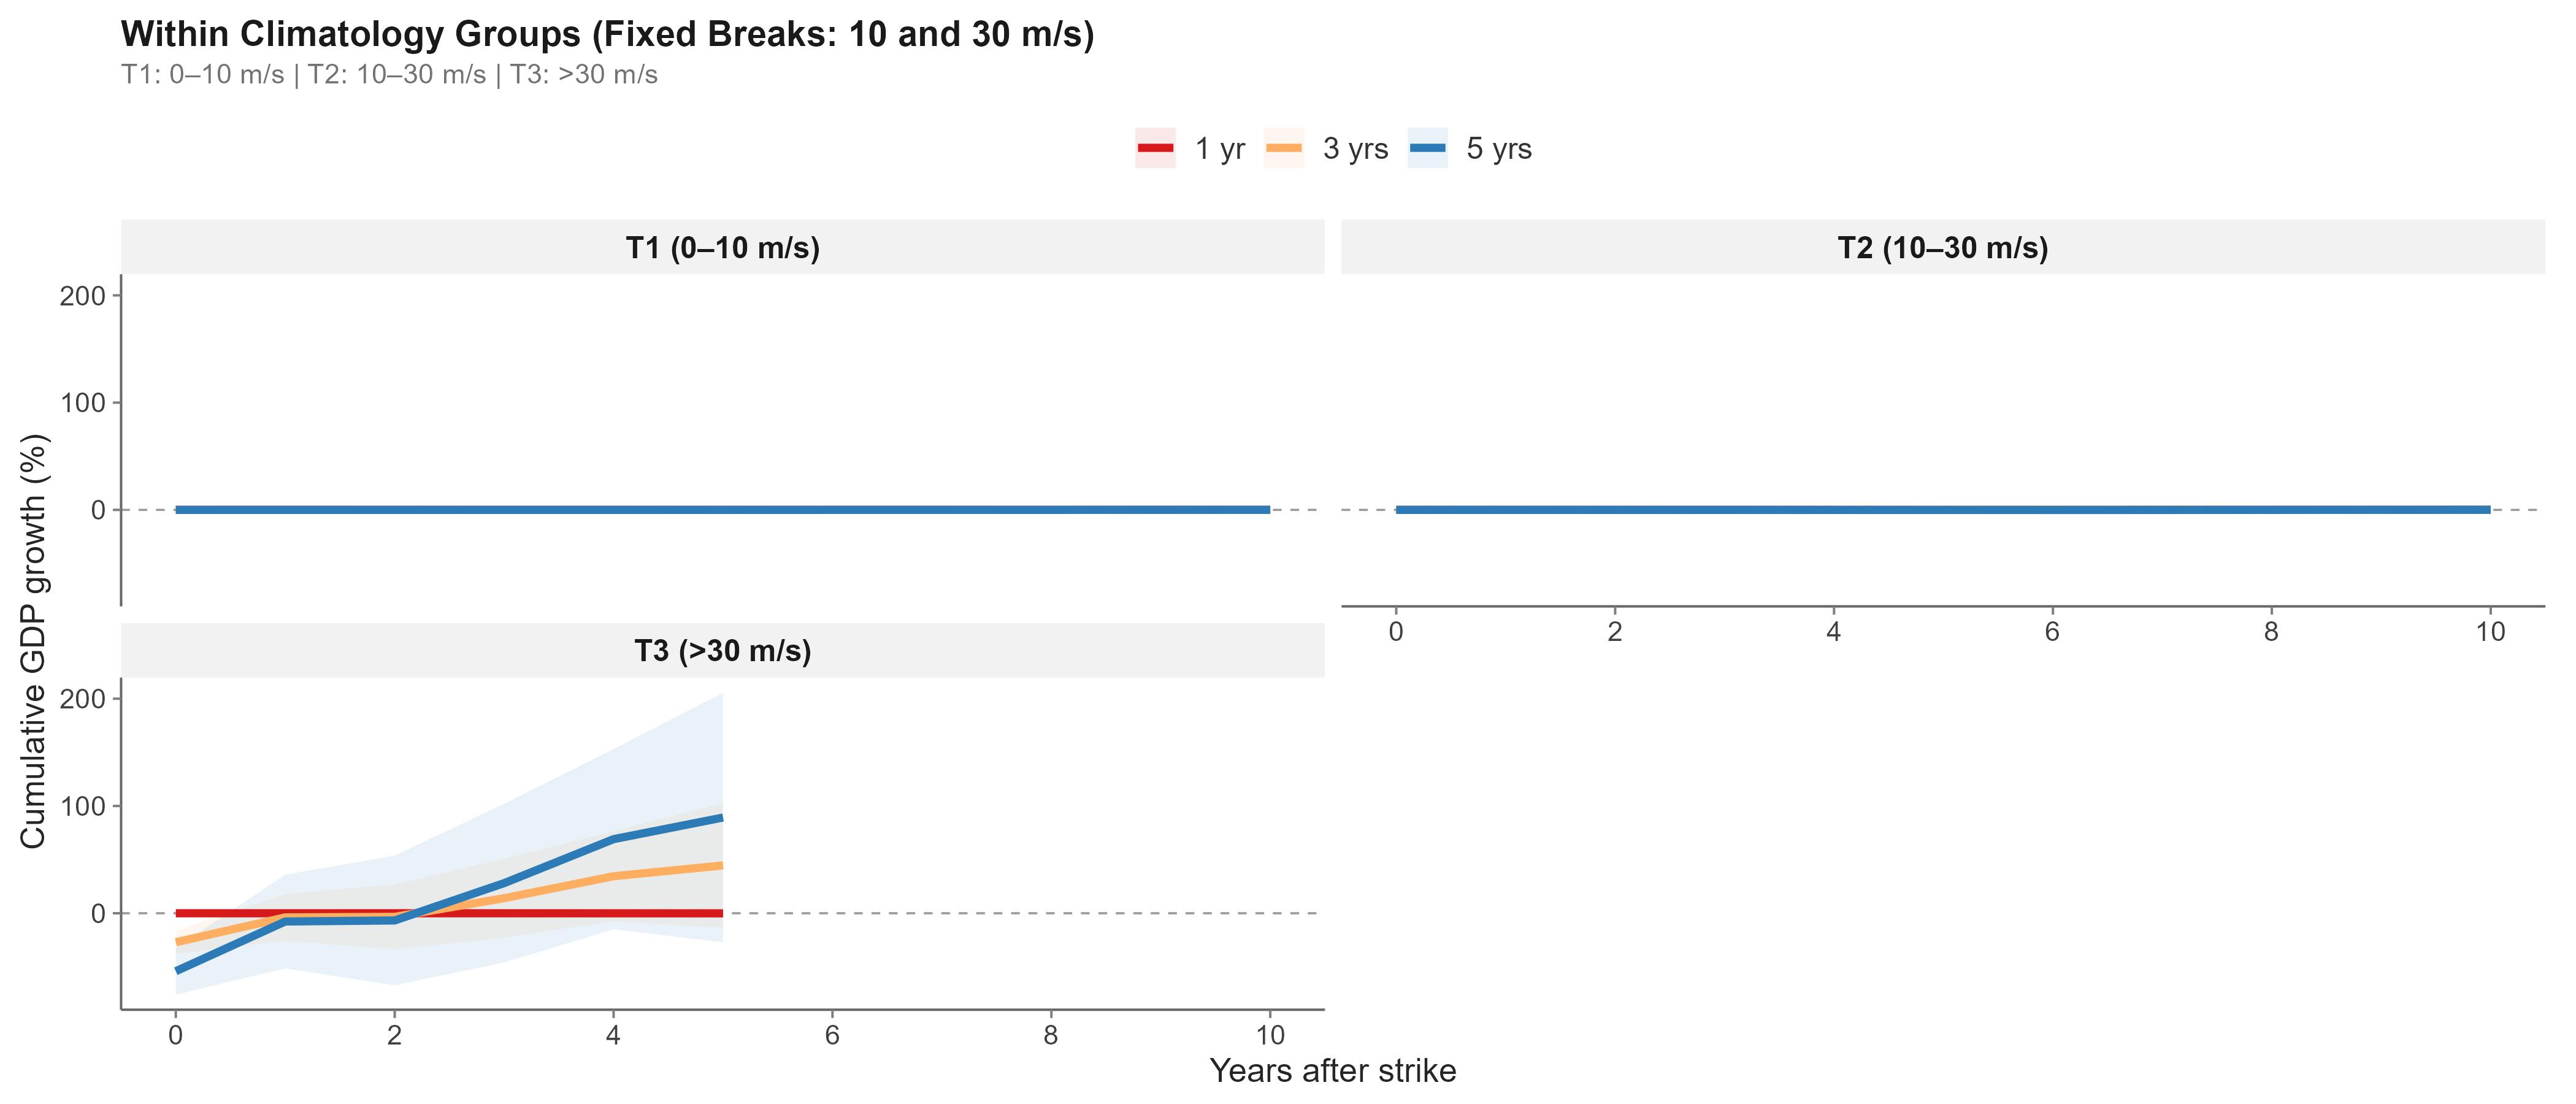
\includegraphics[width=0.96\textwidth,height=0.68\textheight,keepaspectratio]{figures/compound_rob_clim_terciles.png}

\smallskip\small
T1 (0--10\,m/s, $\tau$ mean\,=\,9 yrs, 58\,\% isolated): gradient flat, near zero.
T2 (10--30\,m/s, $\tau$ mean\,=\,1.6 yrs, 85\,\% compound): minimal $\tau$ variation, gradient poorly identified.
T3 ($>$30\,m/s): 100\,\% $\tau\leq2$ --- LP extrapolates wildly ($\hat{\text{gradient}}=89$\,pp), excluded from summary.
\end{frame}

\begin{frame}{Key Test: Residualise $\tau$ on $\bar{W}$}
\centering
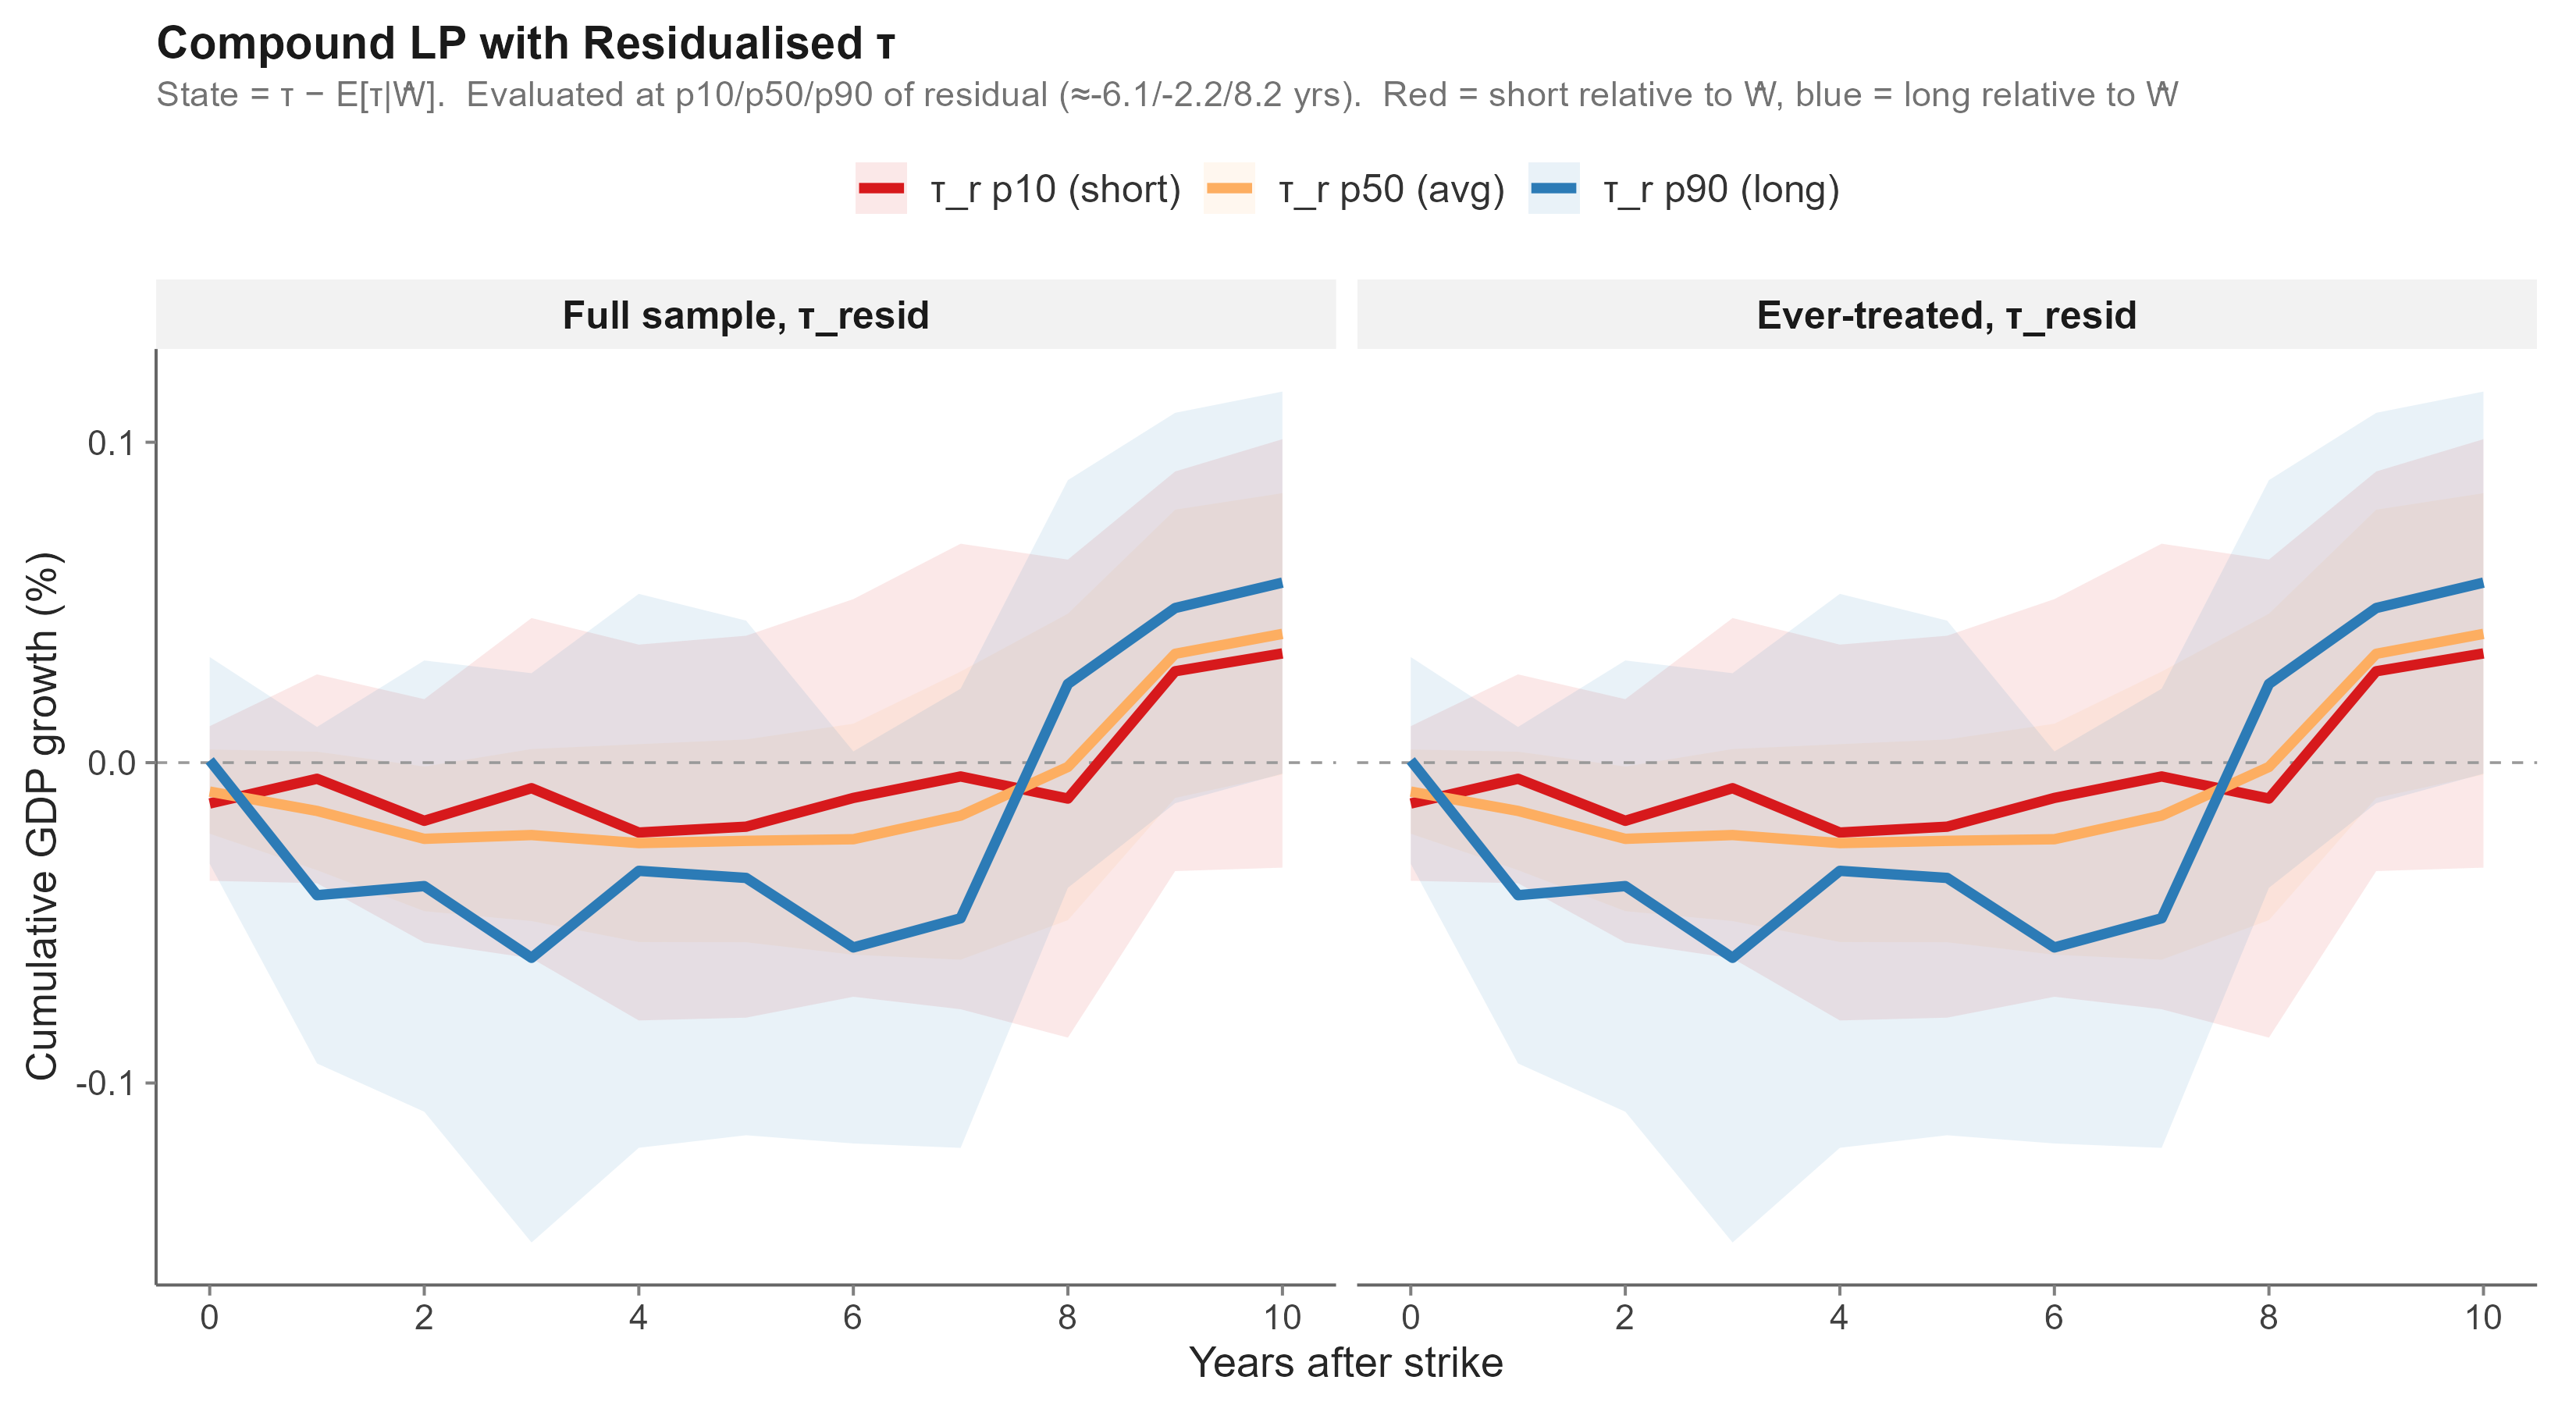
\includegraphics[width=0.96\textwidth,height=0.66\textheight,keepaspectratio]{figures/compound_rob_tau_resid.png}

\smallskip\small
State variable = $\hat\tau_{\text{resid}} = \tau_{it} - \hat{E}[\tau_{it}\mid\bar{W}_i]$
(OLS projection; $\text{cor}(\bar{W},\hat\tau_{\text{resid}})=0$ by construction).
Evaluated at p10 / p50 / p90 of residual ($\approx-6$, $-2$, $+8$ yrs).
\textbf{The gradient is indistinguishable from zero} ($-2$ pp, CI: $[-12,+8]$).
Removing the $\bar{W}$--$\tau$ correlation kills the compound effect.
\end{frame}

\begin{frame}{Gradient Summary: the Compound Effect Is a $\bar{W}$ Confound}
\centering
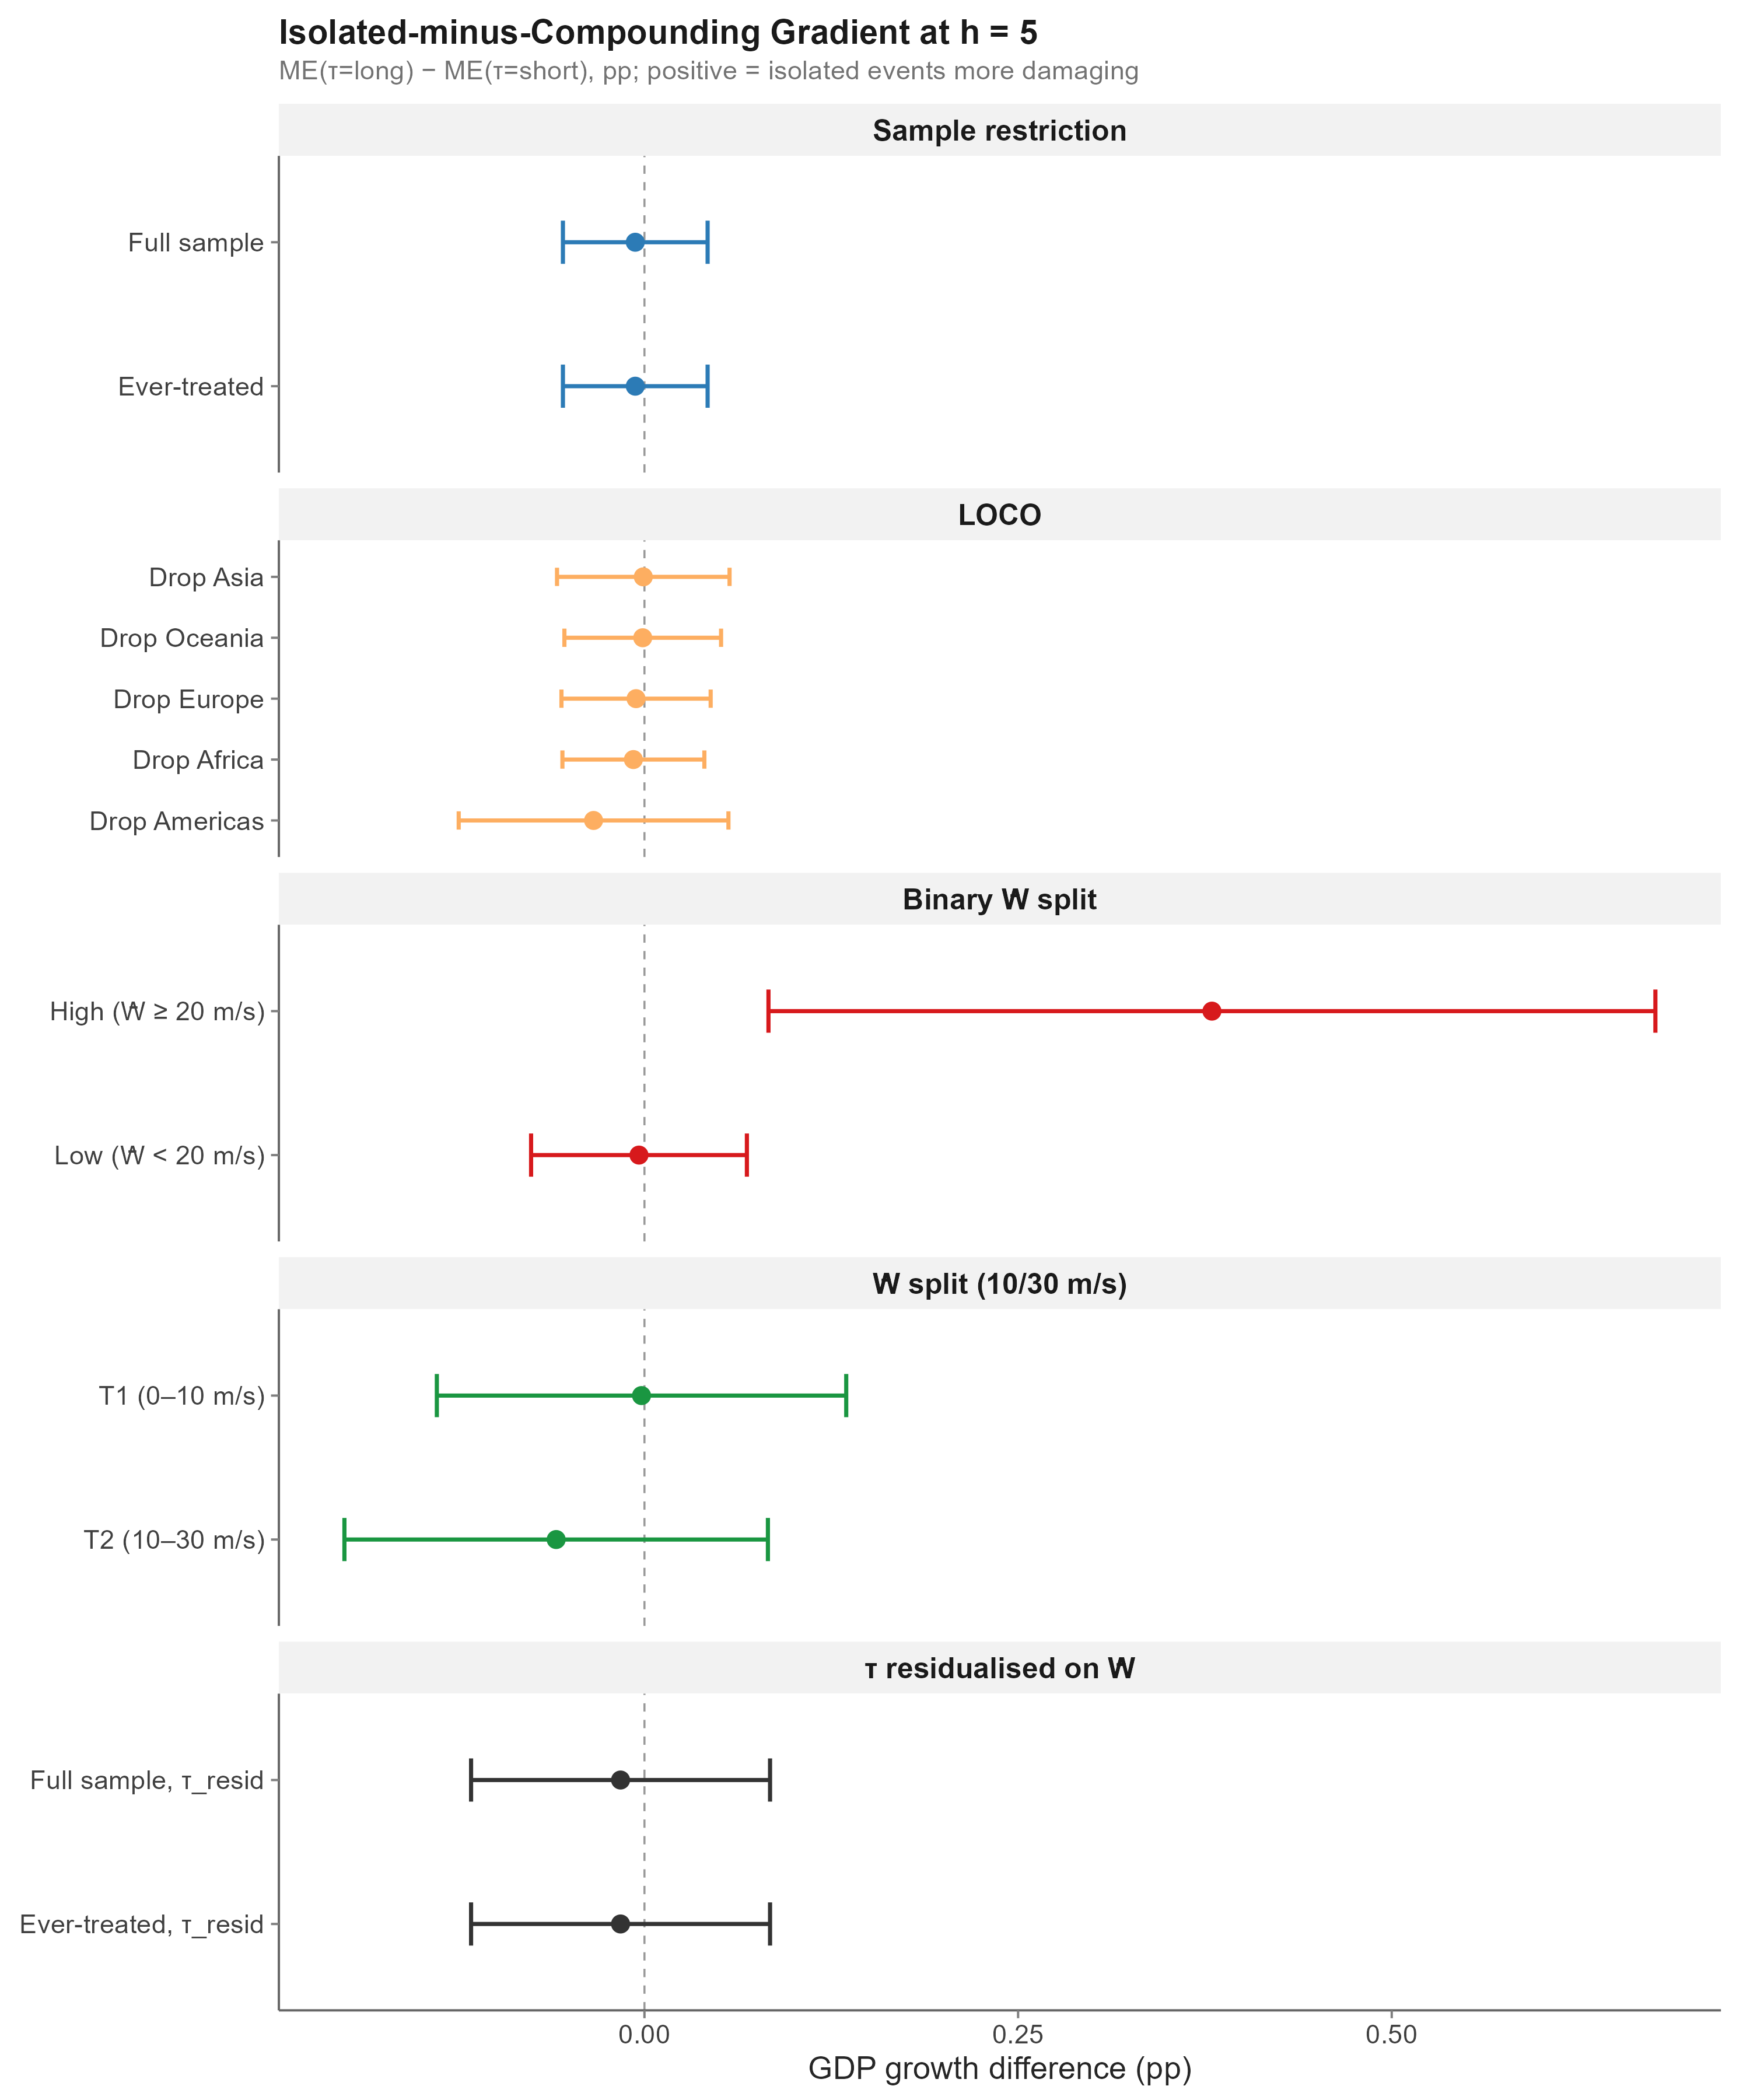
\includegraphics[width=0.60\textwidth,height=0.72\textheight,keepaspectratio]{figures/compound_rob_gradient.png}

\smallskip\small
ME(long\,$\tau$) $-$ ME(short\,$\tau$) at $h=5$.
Positive in full-sample and LOCO tests; collapses to zero in T1 and T2
(10/30\,m/s breaks) and in the residualised-$\tau$ LP.
T3 ($>$30\,m/s) excluded: 100\,\% $\tau\leq2$, LP extrapolates.
The compound gradient is \textbf{a $\bar{W}$--$\tau$ confound}.
\end{frame}

\begin{frame}{ENSO and Climate Controls}
\centering
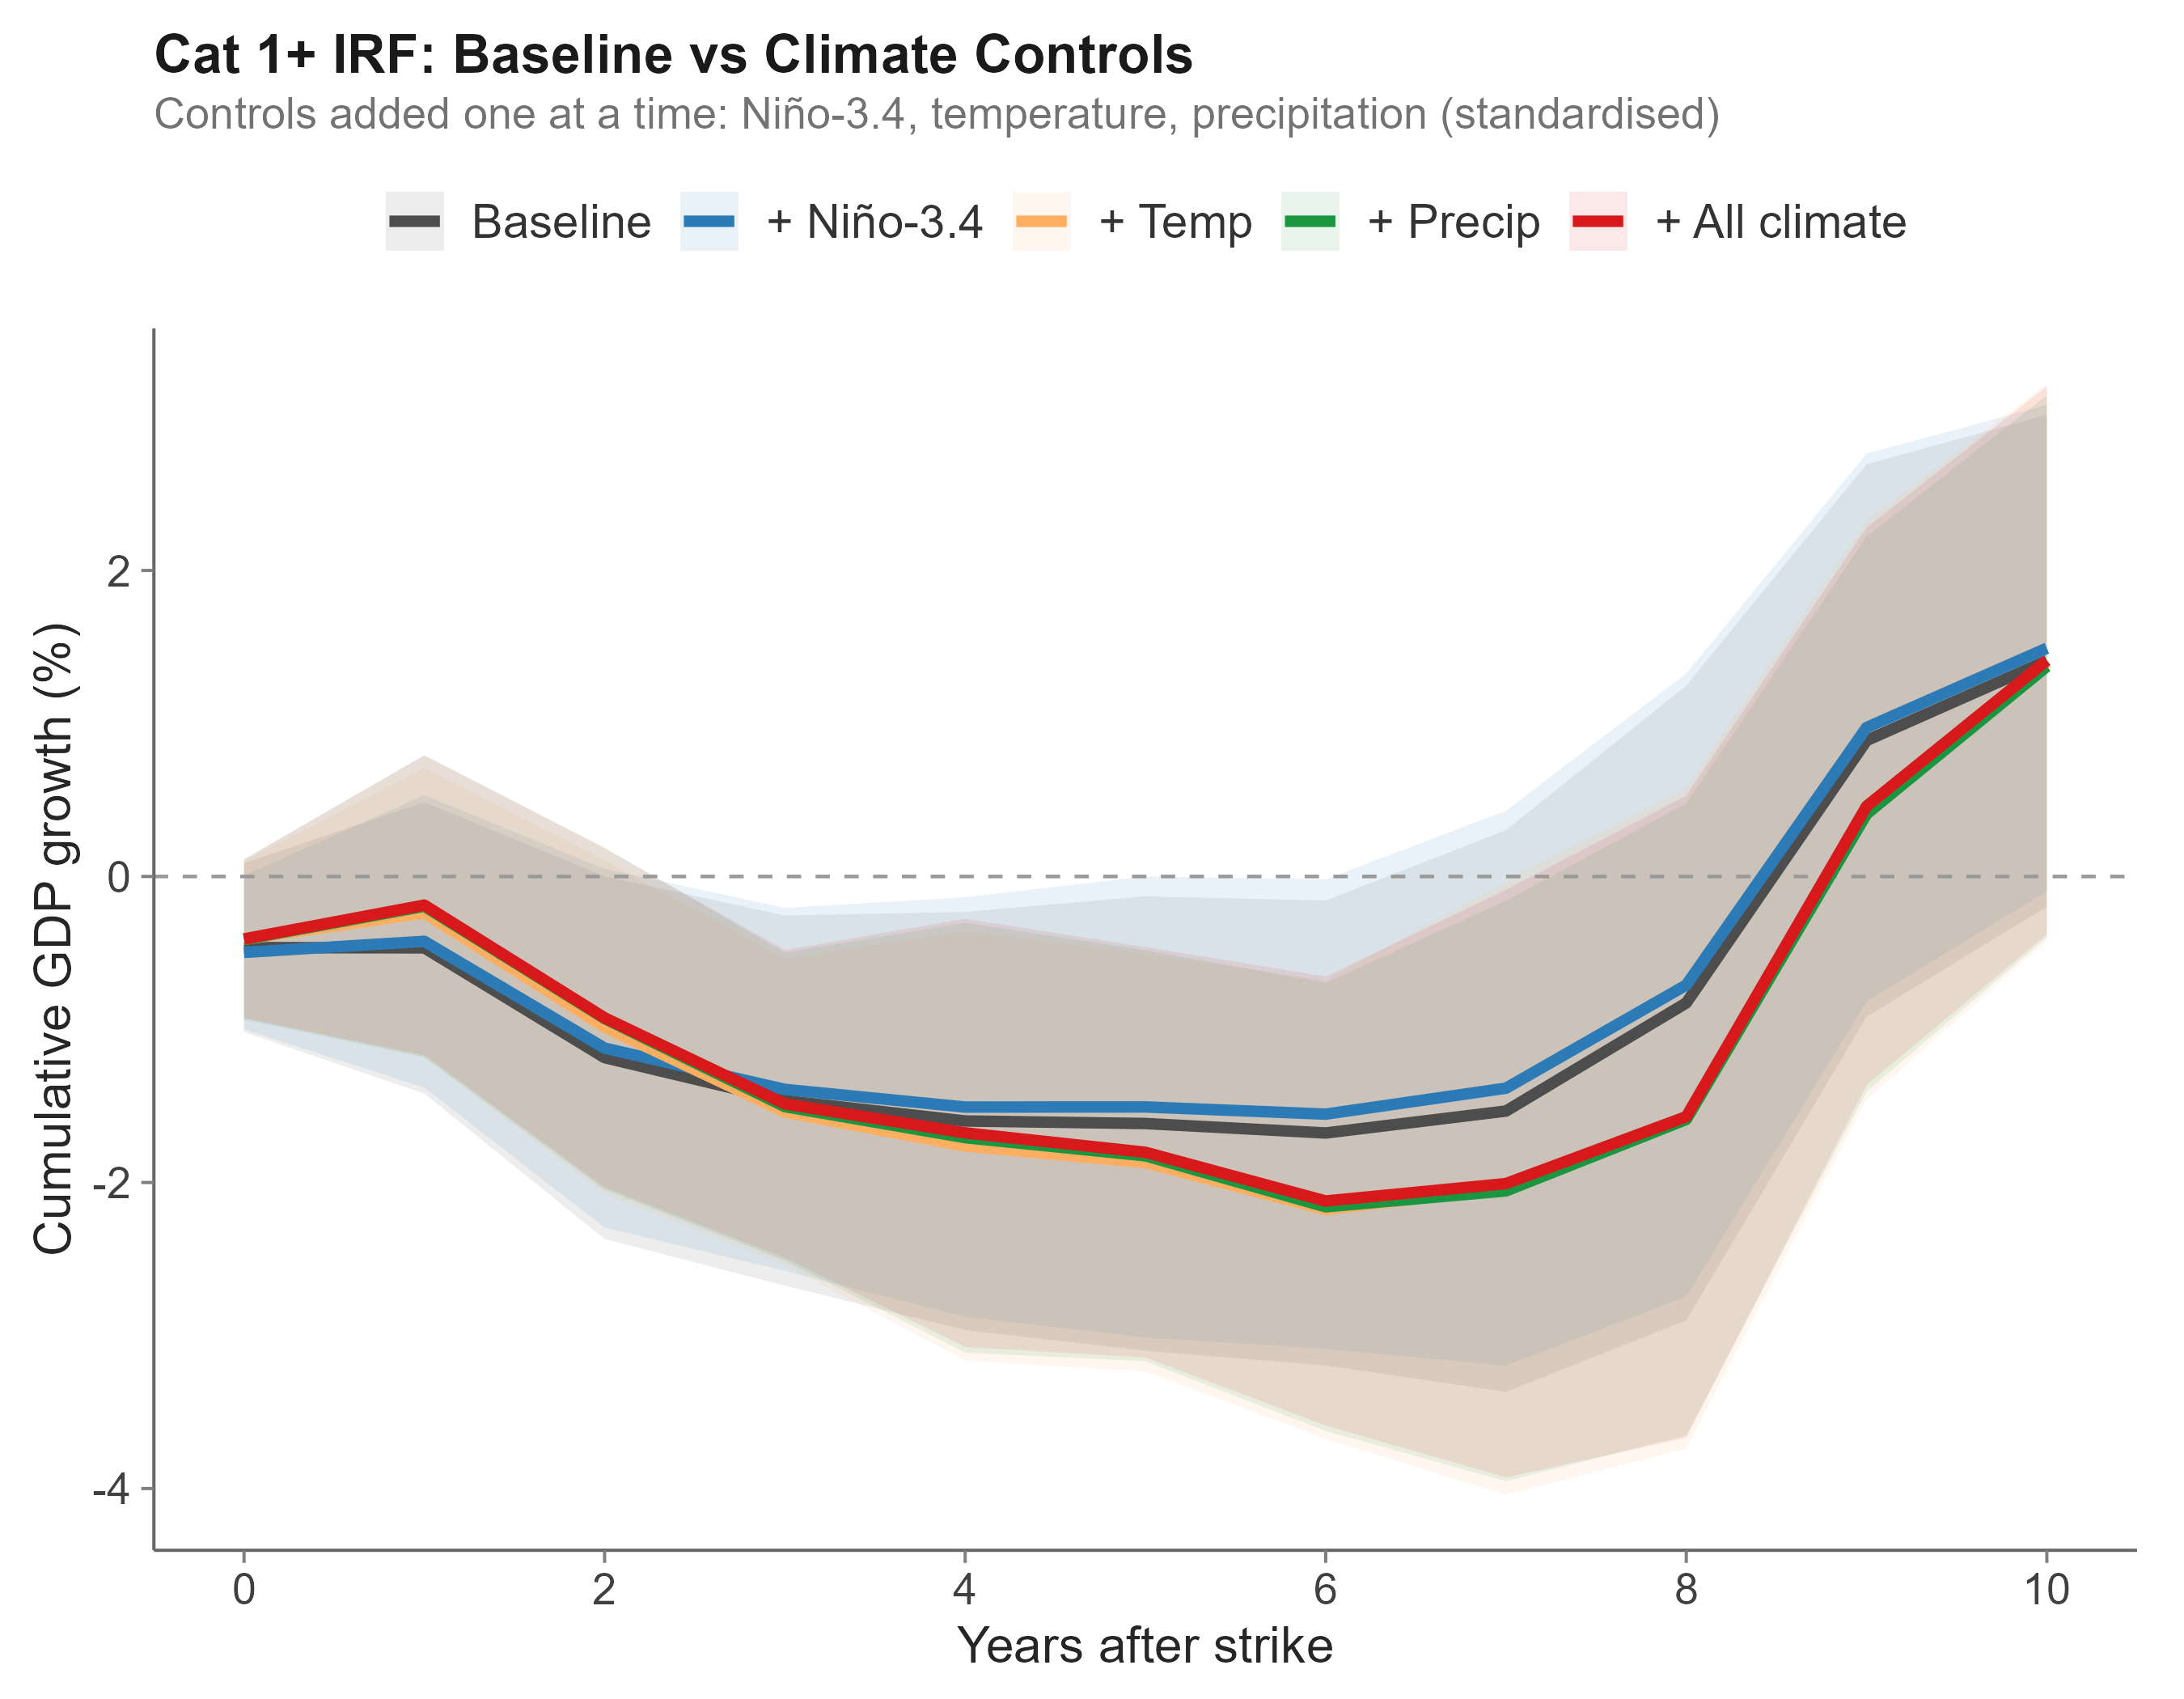
\includegraphics[width=0.88\textwidth,height=0.72\textheight,keepaspectratio]{figures/irf_enso_controls.png}

\smallskip\small
Cat\,1+ baseline LP vs adding Ni\~no-3.4, temperature, and precipitation anomalies
(standardised) as contemporaneous controls.  GDP effect is stable across
specifications $\Rightarrow$ omitted climate variables do not explain the
cyclone--GDP response, strengthening the causal interpretation of $\beta_1$.
\end{frame}

% ===============================================================
\section{Remedies: Towards Valid Identification of $\tau$}
% ===============================================================
{\hideframenumber\begin{frame}\sectionpage\end{frame}\showframenumber}

\begin{frame}{What Would a Valid Instrument for $\tau$ Look Like?}
\small
\textbf{Goal:} instrument $Z_{it}$ satisfying (i) \textbf{relevance}: shifts
$\tau_{it}$, and (ii) \textbf{exclusion}: affects GDP only via $\tau_{it}$.

\smallskip
\begin{tabular}{@{}p{4cm}p{4.2cm}p{3.6cm}@{}}
\toprule
Instrument & Relevance & Exclusion concern \\
\midrule
Basin-wide TC count in $t-1$ (excl.\ own country) &
  High-activity year $\Rightarrow$ $\tau\downarrow$ &
  SST co-moves with agriculture \\[4pt]
ENSO state at $t-1$ (La Ni\~na $\Rightarrow$ more Atlantic TCs) &
  Shifts prior-year strike probability &
  ENSO directly affects rainfall and output \\[4pt]
Lagged strike in adjacent country &
  Regional TC systems hit neighbours in sequence &
  Common regional shocks \\
\bottomrule
\end{tabular}

\smallskip
None of the candidates is clean.  The most promising direction is a
\textbf{shift-share} design: basin-level TC frequency (the ``shift'')
$\times$ country geographic exposure share (time-invariant ``share'').
The share is predetermined and the shift is driven by large-scale
atmospheric dynamics that are plausibly orthogonal to any individual
country's GDP path.
\normalsize
\end{frame}

\begin{frame}{Practical Partial Remedies (Without a Full IV)}
\small
\begin{enumerate}
  \item \textbf{Within-group estimation:} narrow the $\bar{W}$ bins (terciles,
        quartiles) to minimise the within-cell $\tau$--$\bar{W}$ correlation.
        Residual variation in $\tau$ within fine bins is closer to exogenous.

  \smallskip
  \item \textbf{Residualise $\tau$ on $\bar{W}$:} project $\tau_{it}$ on
        $\bar{W}_i$ (or a flexible function) and use the residual as the
        state variable.  Removes cross-sectional correlation while retaining
        within-country variation in inter-strike timing.

  \smallskip
  \item \textbf{Matched sample:} match high-$\tau$ and low-$\tau$ observations
        on $\bar{W}$ and income (CEM).  Compare within matched pairs.

  \smallskip
  \item \textbf{Bounds:} derive worst-case bounds on $\beta_2$ under the
        assumption that all $\tau$ confounding operates through $\bar{W}$
        (Manski-type partial identification).
\end{enumerate}

\smallskip
\textit{Given the results below, the first priority is the residualised-$\tau$
approach: it is implementable, already estimated, and shows the compound
gradient is a $\bar{W}$ confound.}
\normalsize
\end{frame}

% ===============================================================
\section{Takeaways}
% ===============================================================
{\hideframenumber\begin{frame}\sectionpage\end{frame}\showframenumber}

\begin{frame}{Summary}
\small\vspace{-2pt}
\begin{enumerate}
  \item \textbf{Maxwind is plausibly quasi-random conditional on $\bar{W}$.}
        Near-zero ACF supports the i.i.d.\ assumption; ENSO controls do not
        attenuate the GDP effect, supporting causal interpretation of $\beta_1$.

  \item \textbf{$\tau$ is not randomly assigned.}
        High-$\bar{W}$ countries are struck more often $\Rightarrow$ shorter $\tau$
        by construction.  Within the High group (W\={}\,$\geq$20), 98.5\,\% of
        observations have $\tau\leq2$ --- $\tau$ is essentially a constant there.

  \item \textbf{The apparent compound gradient is a $\bar{W}$ confound.}
        Within-$\bar{W}$ terciles T1 and T2, the gradient is zero.
        Once $\tau$ is residualised on $\bar{W}$ (removing the cross-country
        level correlation), the gradient collapses to $-2$\,pp and is
        statistically indistinguishable from zero (CI: $[-12,+8]$).

  \item \textbf{``Within climatology groups'' is not a valid fix.}
        The High group has near-degenerate $\tau$ variation, so the LP
        extrapolates rather than identifies.  The apparent gradient in High
        is an artefact of that extrapolation.

  \item \textbf{Conclusion:} no evidence that time since last TC
        causally moderates the GDP response once the $\bar{W}$--$\tau$
        mechanical link is controlled for.  A valid IV (shift-share:
        basin TC count $\times$ country exposure share) would provide
        a definitive test.
\end{enumerate}
\normalsize
\end{frame}

\end{document}
